%% --------------------------------------------------------------------
%% Template UTEC Tesis
%% --------------------------------------------------------------------
% Este es el archivo que se debe compilar.
% 
% Este template ha sido modificado y actualizado por Eduardo Castro y Roosevelt Ubaldo sobre la base de lo trabajado por Víctor Murray, Oscar Ramos y Juan Carlos Barbaran.
%
% Última actualización: Marzo, 2026

\documentclass[a4paper,12pt,oneside]{tesisutec}

\selectlanguage{spanish}

%% Paquetes

\usepackage{tabularx}
\usepackage{xltabular}
\usepackage{booktabs}
\usepackage[utf8]{inputenc}
\usepackage[square, numbers, comma, sort&compress]{natbib}
% Libreria de idioma
\usepackage[spanish]{babel}
% Libreria para posicionamiento
\usepackage{float}
% Librerias para insertar codigos
\usepackage[spanish,onelanguage,ruled,vlined]{algorithm2e}
\usepackage{verbatim} 
% Librería para hipervínculos
\usepackage{hyperref}
 % Librería necesaria para arreglar el orden de referencias en overleaf.com
\usepackage{notoccite}
\usepackage{tikz}
\usetikzlibrary{positioning}

% Incluir acá los paquetes adicionales que deseas. 
% Ubicación de los imágenes.
\graphicspath{images/}

\makeatletter
% Reinsert missing \algbackskip
\def\algbackskip{\hskip-\ALG@thistlm}
\makeatother

\hypersetup{urlcolor=blue, colorlinks=true}

\begin{document}

\frontmatter

\department{BIOINGENIERÍA}
\degree{Bioingeniería}
\major{Bachiller}

\title{Diseño de un modelo predictivo de riesgo de deterioro de la Estela de Raimondi basado en genómica comparativa y potencial metabólico}

\author{\centering Eduardo Esteban Tello Osorio \orcid{0009-0003-1365-2577} \\
Ana Sofía Barrientos Uriarte \orcid{0009-0006-0570-552X}} % Es obligatorio agregar ORCID del alumno

\supervisor{ Pablo Tsukayama Cisneros \orcid{0000-0002-1669-2553} 
\\
Monica Cecilia Santa María Fuster \orcid{0000-0003-4789-7444}
\\
Harry Gustavo Saavedra Espinoza \orcid{0000-0002-8896-5020}}% Es obligatorio agregar ORCID del asesor

\date{2026}

\maketitle

\setstretch{1.5}


%%% ============================================================================
%  Dedicatoria
%% ============================================================================

\dedicatory{
xxxxxxxxxxxxxxxxxxxxxxxxxxxxxxxxxxxxxxxxxxxxxxxxxxx
xxxxxxxxxxxxxxxxxxxxxxxxxxxxxxxxxxxxxxxxxxxxxxxxxxx
xxxxxxxxxxxxxxxxxxxxxxxxxxxxxxxxxxxxxxxxxxxxxxxxxxx
xxxxxxxxxxxxxxxxxxxxxxxxxxxxxxxxxxxxxxxxxxxxxxxxxxx
xxxxxxxxxxxxxxxxxxxxxxxxxxxxxxxxxxxxxxxxxxxxxxxxxxx
XXxxxxxxxxxxxxxxxxxxxxxxxxxxxxxxxxxxxxxxxxxxxxxxxx
}

%%% ============================================================================
%  Pagina de Agradecimientos
%% ============================================================================

\acknowledgements{

xxxxxxxxxxxxxxxxxxxxxxxxxxxxxxxxxxxxxxxxxxxxxxxxxxx
xxxxxxxxxxxxxxxxxxxxxxxxxxxxxxxxxxxxxxxxxxxxxxxxxxx
xxxxxxxxxxxxxxxxxxxxxxxxxxxxxxxxxxxxxxxxxxxxxxxxxxx
xxxxxxxxxxxxxxxxxxxxxxxxxxxxxxxxxxxxxxxxxxxxxxxxxxx
xxxxxxxxxxxxxxxxxxxxxxxxxxxxxxxxxxxxxxxxxxxxxxxxxxx
xxxxxxxxxxxxxxxxxxxxxxxxxxxxxxxxxxxxxxxxxxxxxxxxxxx

}



\tableofcontents

\newpage

\listoftables

\newpage

\listoffigures

\addtocontents{toc}{\vspace{1.5em}}

%% ============================================================================
\mainmatter
\pagestyle{fancy}

\customchapter{RESUMEN}
\noindent
El patrimonio pétreo está expuesto al biodeterioro microbiano, proceso mediante el cual las comunidades que colonizan la roca disuelven su matriz mineral y alteran su superficie. La Estela de Raimondi, litoescultura de granito de la cultura Chavín bajo custodia museística, presenta biopelículas y alteraciones cromáticas cuya evaluación previa se limitó a la identificación taxonómica, sin esclarecer la capacidad de deterioro de los organismos vivos que la habitan. El objetivo de este proyecto fue diseñar un flujo de análisis computacional para caracterizar el potencial de biodeterioro y las señales de adaptación genómica de los linajes bacterianos dominantes de la fracción viable del monumento, con el fin de sustentar la evaluación del riesgo y una conservación preventiva basada en evidencia genómica. Se partió de datos de secuenciación metagenómica masiva obtenidos de la fracción cultivable de la superficie, sobre los que se estructuró un flujo reproducible que integró el control de calidad genómica, la clasificación taxonómica basada en el genoma completo, la agrupación de genomas redundantes en linajes, la reconstrucción pangenómica comparativa frente a referencias globales y la anotación funcional del potencial metabólico.\\


\noindent \textbf{Palabras clave:}\\
\noindent Biodeterioro; Patrimonio pétreo; Metagenómica; Pangenoma;
Potencial metabólico; Conservación preventiva; Estela de Raimondi
\customchapter{ABSTRACT} 


Stone heritage is exposed to microbial biodeterioration, a process by which the communities colonizing the rock dissolve its mineral matrix and alter its surface. The Raimondi Stela, a granite lithosculpture of the Chavín culture held in a national museum, exhibits biofilms and chromatic alterations whose prior assessment was limited to taxonomic identification, without clarifying the deterioration capacity of the living organisms inhabiting it. The objective of this project was to design a computational analysis workflow to characterize the biodeterioration potential and the genomic adaptation signals of the dominant bacterial lineages of the monument's viable fraction, in order to support risk assessment and genomics-based preventive conservation. High-throughput metagenomic sequencing data obtained from the cultivable surface fraction were used as the starting point, upon which a reproducible workflow was structured, integrating genomic quality control, whole-genome-based taxonomic classification, the grouping of redundant genomes into lineages, comparative pangenomic reconstruction against global references, and functional annotation of metabolic potential.  \\


\noindent \textbf{Keywords:}\\
\noindent  Biodeterioration; Stone heritage; Metagenomics; Pangenome;
Metabolic potential; Preventive conservation; Raimondi Stela


 
\chapter{INTRODUCCIÓN} 

\introsection{Presentación del proyecto}

La Estela de Raimondi es una de las piezas más importantes de la cultura Chavín (Horizonte Temprano, 1200 a.C. - 400 a.C.) y un pilar de la arqueología andina. Elaborada en granito pulido, esta litoescultura de casi dos metros de altura representa a una divinidad antropomorfa, el ``Dios de los Báculos'', caracterizada por una compleja iconografía que integra rasgos de felinos, aves de rapiña y serpientes \cite{cordycollins1993}. Tras su hallazgo a mediados del siglo XIX, inicialmente por el agricultor Timoteo Espinoza en 1840 y su posterior reconocimiento valórico por Antonio Raimondi en 1860 en el Templo Nuevo de Chavín de Huántar, la Estela ha sido objeto de múltiples traslados y, por consiguiente, daños, desde su uso doméstico en Áncash hasta su actual custodia en el Museo Nacional de Arqueología, Antropología e Historia del Perú (MNAAHP) \cite{hernandez2012}.

El presente proyecto de tesis surge de la necesidad de aplicar herramientas de genómica avanzada y bioinformática para entender la ecología microbiana que habita este monumento, integrando el análisis del pangenoma de linajes bacterianos para identificar poblaciones propias de la región, así como para predecir riesgos de deterioro en elementos arqueológicos.

\introsection{Descripción de la situación problemática}

A pesar de encontrarse en un ambiente controlado de museo, la Estela de Raimondi no es inmune al paso del tiempo ni a la interacción con agentes biológicos. Históricamente, la pieza ha sufrido daños físicos, incluyendo fracturas por el terremoto de 1940 \cite{mnaahp2015}. Sin embargo, informes técnicos recientes han identificado la presencia de biopelículas y alteraciones cromáticas en la superficie del granito.

Las piedras arqueológicas, como la caliza, el granito o la toba volcánica, son altamente susceptibles al daño causado por comunidades microbianas, incluyendo bacterias, cianobacterias, algas y hongos. Los microorganismos penetran los poros y fisuras de la piedra mediante hifas fúngicas o forman biopelículas \cite{dakal2012}. Estas comunidades pueden inducir biocorrosión mediante la secreción de ácidos orgánicos que disuelven la matriz mineral o generar pigmentos que alteran irreparablemente la estética del monumento \cite{dakal2012,villa2016}. Sin embargo, se ha demostrado que las biopelículas subaéreas tienen un rol dual, pues mientras algunas causan deterioro, otras pueden actuar como una capa bioprotectora que regula la humedad térmica, consolida la superficie y protege a la piedra de los contaminantes atmosféricos \cite{villa2016,alonso2025}.

El problema reside en que las estrategias tradicionales de conservación suelen ser reactivas y basadas en identificación taxonómica básica, ignorando el potencial metabólico real, las poblaciones favorables y las capacidades adaptativas de las bacterias que dominan la biopelícula.

\introsection{Formulación del problema}

Si bien estudios previos sobre la Estela de Raimondi permitieron caracterizar la diversidad taxonómica de su microbioma mediante secuenciación de amplicones (16S rRNA e ITS2) a partir de ADN ambiental, esta aproximación presenta limitaciones importantes para evaluar su papel en el biodeterioro del monumento. Por un lado, el ADN ambiental no permite distinguir entre microorganismos metabólicamente activos, latentes o muertos, ni diferenciar a los verdaderos colonizadores del sustrato de aquellos microorganismos depositados pasivamente desde el ambiente ~\cite{skipper2022,branysova2022}. Por otro lado, la secuenciación de amplicones ofrece información sobre la identidad taxonómica de la comunidad microbiana, pero no permite determinar su potencial metabólico ni las capacidades adaptativas de las poblaciones presentes ~\cite{PitaGaleana2025}.

Frente a ello, la presente tesis se concentra en la fracción viable del microbioma, es decir, en aquellos microorganismos capaces de crecer en cultivo y, por tanto, confirmados como vivos. A partir de esta fracción se realizó secuenciación metagenómica \textit{shotgun}~\cite{tsukayama2025informe}. Mediante el ensamblaje de genomas metagenómicos (MAGs) y el análisis comparativo de sus genes accesorios frente a referencias globales, se busca caracterizar el potencial metabólico y las señales de adaptación evolutiva de los linajes bacterianos dominantes en el sustrato lítico. Esta aproximación permite identificar biomarcadores genómicos asociados a la producción de ácidos y a la formación de biopelículas, aportando parámetros técnicos para la evaluación del riesgo de biodeterioro y el diseño de protocolos de conservación preventiva basados en evidencia genómica.

\introsection{Objetivos del proyecto}

\introsection{Objetivo general}

Diseñar un modelo predictivo para determinar el potencial metabólico y la evolución genómica de los linajes bacterianos dominantes en la Estela de Raimondi mediante análisis de pangenoma y potencial metabólico.

%Caracterizar el potencial de biodeterioro y las señales de adaptación genómica de los linajes bacterianos dominantes de la fracción viable de la Estela de Raimondi, mediante el análisis pangenómico comparativo y la reconstrucción de su potencial metabólico frente a genomas de referencia globales.

\introsection{Objetivos específicos}

\begin{enumerate}
    \item Seleccionar los MAGs con mayor integridad ($>70\%$) y baja contaminación ($<5\%$).
    \item Determinar la posición filogenómica de los MAGs seleccionados mediante el cálculo de ANI (Identidad Nucleotídica Promedio) y filogenia frente a bases de datos internacionales como NCBI y GTDB.
    \item Definir el genoma core y el genoma accesorio de los linajes dominantes de la fracción viable de la Estela frente a genomas de referencia globales, identificando genes exclusivos, es decir, específicos de la Estela.
    \item Mapear las rutas metabólicas de supervivencia, como la esporulación, y de deterioro, como la formación de biopelículas y la producción de ácidos, analizando si los genes responsables se encuentran en el genoma accesorio, es decir, si fueron adquiridos por adaptación al monumento.
\end{enumerate}

\introsection{Justificación}

El presente trabajo surge de la necesidad de transitar de una caracterización taxonómica convencional hacia un análisis de resolución genómica. En el contexto de la conservación del patrimonio en Latinoamérica, los estudios microbiológicos suelen detenerse en la descripción de géneros, dejando sin respuesta la interrogante sobre qué mecanismos biológicos específicos están siendo ejecutados activamente en la superficie del monumento \cite{villa2016,alonso2025}. El uso de bioinformática avanzada para la reconstrucción de MAGs y el análisis pangenómico permitirá identificar si los determinantes de biodeterioro, como la síntesis de ácidos orgánicos o la formación de biopelículas, son rasgos intrínsecos de los linajes o adaptaciones adquiridas para la supervivencia en el monumento \cite{skipper2022,jroundi2020}. Este estudio no solo posiciona el análisis del patrimonio cultural peruano a la vanguardia tecnológica regional, sino que provee una base científica para predecir riesgos y optimizar estrategias de conservación preventiva menos invasivas.

\introsection{Alcance y limitaciones}

El alcance de esta tesis es de naturaleza estrictamente computacional y descriptiva, basándose en el análisis de datos metagenómicos previamente secuenciados de la Estela de Raimondi por la Universidad Peruana Cayetano Heredia (Laboratorio de Genómica Microbiana). El estudio se centrará exclusivamente en los linajes bacterianos dominantes que presenten métricas de calidad genómica adecuadas para un análisis pangenómico robusto.

Entre las limitaciones, se debe precisar que la caracterización
describe la fracción del microbioma recuperable mediante cultivo, que corresponde a un
subconjunto de la comunidad viable y no necesariamente a la totalidad de las
poblaciones dominantes \textit{in situ}~\cite{sterflinger2013,branysova2022}. A cambio,
garantiza que los genomas analizados provienen de organismos vivos, condición necesaria
para atribuirles un rol activo en el biodeterioro. Asimismo, al no contar con datos de metatranscriptómica (RNA-seq), la caracterización funcional representa el potencial metabólico y no la actividad biológica real en el momento de la toma de muestra \cite{cappitelli2020}. Además, la integridad y el grado de contaminación de los MAGs están intrínsecamente ligados a la profundidad de la secuenciación original y a la complejidad de la biopelícula colonizadora \cite{villa2016,checkm2}. Por otro lado, la potencia del análisis pangenómico está sujeta a la disponibilidad y representatividad de genomas de referencia de alta calidad en bases de datos globales como NCBI o GTDB \cite{gtdbtk2019}. Finalmente, factores abióticos externos, como las fluctuaciones de humedad y temperatura en el museo, solo se utilizarán como marco contextual para interpretar las estrategias de supervivencia microbiana.
\chapter{ESTADO DEL ARTE}
\label{chap:estado_arte}

A lo largo del tiempo, la evaluación del biodeterioro en monumentos arqueológicos e históricos ha pasado por distintas etapas tecnológicas, donde cada método presentó limitaciones operativas y alcances técnicos que influyeron en la evolución del área. En este contexto, el propósito de este capítulo es revisar de manera crítica las soluciones analíticas y de intervención desarrolladas tanto en el ámbito académico como industrial, estableciendo un marco comparativo basado en parámetros de rendimiento, cobertura y viabilidad técnica. Esto permitirá comprender las fortalezas y limitaciones de los enfoques previos, así como justificar el desarrollo y la adopción de aproximaciones diagnósticas contemporáneas. 

\section{Soluciones precedentes}
\label{sec:soluciones_precedentes}
\subsection{Protocolos basados en cultivo microbiológico (método tradicional)}
\label{subsec:cultivo_tradicional}
Durante décadas, el estudio de los ecosistemas microbianos en el patrimonio pétreo dependió casi exclusivamente de técnicas dependientes de cultivo. Las muestras extraídas del sustrato se sembraban en medios de laboratorio generales, como Agar Nutritivo, MEA o PDA, frecuentemente suplementados con antibióticos o cicloheximida para la selección de grupos específicos \cite{branysova2022}. Este enfoque permitió aislar e identificar morfológicamente a numerosos taxa bacterianos y fúngicos asociados al biodeterioro.

No obstante, esta metodología introduce sesgos selectivos, siendo su principal limitación la estructural: se estima que aproximadamente el 99 \% de los microorganismos ambientales son "viables pero no cultivables" (VBNC) en condiciones de laboratorio estándar, dado que los medios artificiales no replican las condiciones oligotróficas, de estrés hídrico y radiación UV características de las superficies pétreas \cite{branysova2022, sterflinger2013, suchy2024}. En contraste con las tecnologías moleculares modernas, los métodos de cultivo solo logran detectar entre el 1 \% y el 5 \% de la comunidad microbiana total \cite{li2018deterioration}. Un estudio ilustrativo realizado en el campo de concentración de Auschwitz demostró que el cultivo detectó apenas 8 géneros bacterianos, mientras que la secuenciación NGS reveló 99 géneros en el mismo material \cite{gutarowska2015}. Adicionalmente, los medios de cultivo imponen concentraciones artificialmente elevadas de nutrientes, lo que favorece a microorganismos heterótrofos de rápido crecimiento que pueden no ser los colonizadores dominantes ni los principales agentes de deterioro in situ \cite{branysova2022, zanardini2019}.

Ahora bien, esta misma selectividad adquiere valor metodológico cuando el objetivo no es
inventariar la comunidad total, sino identificar a los organismos con capacidad real de
deterioro. A diferencia del ADN ambiental, que persiste en el sustrato tras la muerte
celular y no distingue entre células activas y muertas ~\cite{branysova2022}, el crecimiento
en cultivo constituye una prueba directa de viabilidad: todo microorganismo aislado está,
por definición, vivo. Por ello, la secuenciación metagenómica aplicada sobre la fracción
cultivada permite acoplar la certeza de viabilidad con la resolución genómica, estrategia
adoptada en la presente tesis~\cite{tsukayama2025informe}. La contrapartida, que se
mantiene explícita, es que dicha fracción representa únicamente el subconjunto cultivable
de la comunidad viable, por lo que sus conclusiones no se extienden a los linajes que no
crecen en los medios empleados.

\subsection{Tratamientos y limpieza con biocidas químicos}
\label{subsec:biocidas_quimicos}

Para el control del biodeterioro, la práctica conservativa tradicional recurrió históricamente a sustancias antimicrobianas de síntesis química: alcoholes, fenoles, aldehídos, compuestos de amonio cuaternario (como el cloruro de benzalconio), sales de estaño, derivados de isotiazolinonas y tratamientos de fumigación con óxido de etileno \cite{sterflinger2013, cappitelli2020}. Estas estrategias presentan ventajas a corto plazo en términos de reducción de biomasa visible, pero exhiben graves inconvenientes a mediano y largo plazo.

En primer lugar, la eficacia del biocida es frecuentemente transitoria y requiere reaplicaciones periódicas \cite{cappitelli2020}. En segundo lugar, generan toxicidad tanto para los operadores humanos como para el ecosistema circundante \cite{cappitelli2020}. Desde el punto de vista material, los biocidas oxidantes pueden inducir manchas por herrumbre y eflorescencias sobre la piedra, mientras que las soluciones de limpieza ácida o alcalina comprometen la integridad mineralógica del sustrato \cite{cappitelli2020}. Finalmente, y de mayor relevancia para la gestión del biodeterioro a largo plazo, los biocidas eliminan el microbioma natural sin remover la biomasa celular residual, la cual actúa como sustrato nutritivo que acelera la recolonización. Bajo la presión selectiva del biocida, las comunidades que recolonizan son frecuentemente resistentes al tratamiento y presentan perfiles metabólicos más agresivos, involucrando tanto a cepas bacterianas resistentes como a una mayor presencia de hongos altamente melanizados \cite{cappitelli2020, gorbushina2007}. Este efecto fue documentado de forma notable tras los tratamientos masivos realizados en las cuevas de Lascaux y en la tumba de San Pablo en Éfeso \cite{sterflinger2013}.

\section{Análisis comparativo de tecnologías actuales}
\label{sec:analisis_molecular_ngs}

La introducción de las tecnologías de secuenciación de próxima generación (NGS) como Illumina MiSeq, NovaSeq, PacBio y Oxford Nanopore, redefinió los estándares del análisis del microbioma del patrimonio pétro. En la práctica contemporánea, coexisten diversos enfoques que compiten en términos de rendimiento de datos, costos operativos y viabilidad de estandarización.

La secuenciación de amplicones de genes marcadores evolutivamente conservados, como las regiones hipervariables V3-V6 del gen 16S rRNA (para bacterias y arqueas) y las regiones ITS1/ITS2 (para hongos), permite la identificación filogenética de alta resolución sin necesidad de cultivo previo \cite{suchy2024, chimienti2016}.

La metagenómica de escopeta (shotgun metagenomics) secuencia la totalidad del material genético presente en la muestra, superando el sesgo de la amplificación específica por PCR y revelando no solo qué organismos están presentes, sino que permite determinar potencialmente qué rutas metabólicas y genes funcionales contiene la comunidad \cite{suchy2024, ding2020preahvihear}. Estudios previos demostraron que la secuenciación de amplicones permite detectar una diversidad microbiana significativamente superior a la obtenida mediante métodos clásicos y, en combinación con herramientas bioinformáticas predictivas, inferir el potencial funcional del microbioma en monumentos pétreos \cite{li2018deterioration, chimienti2016}.

Cabe precisar que la metagenómica \textit{shotgun} puede aplicarse tanto sobre ADN
extraído directamente del ambiente como sobre material previamente enriquecido por
cultivo; en el segundo caso, la comunidad se acota a su fracción viable a cambio de un
ADN de mayor calidad y trazabilidad, un compromiso relevante en muestras de baja biomasa
como las superficies pétreas~\cite{tsukayama2025informe,ding2020}.

En términos comparativos con los métodos tradicionales, la NGS supera significativamente al cultivo en cobertura taxonómica, sensibilidad y representatividad de la comunidad real \cite{sterflinger2013, suchy2024, gutarowska2015}. No obstante, su coste por muestra es considerablemente más elevado, requiere equipamiento especializado, genera grandes volúmenes de datos que demandan análisis bioinformáticos complejos, y presenta limitaciones propias: artefactos genéticos generados durante la amplificación por PCR (secuencias quiméricas), resolución taxonómica que frecuentemente no alcanza el nivel de especie, y dificultades de extracción de ADN en estructuras resistentes como las endosporas de Bacillus spp. \cite{branysova2022, li2018deterioration, skipper2022}.

En la frontera tecnológica se ubican la metatranscriptómica y la metabolómica ambiental, diseñadas para resolver el perfil funcional dinámico del microbioma in situ \cite{cappitelli2020, gutarowska2015}. La metatranscriptómica ofrece la medición directa de los transcritos de ARN activos al momento del muestreo, discriminando con precisión entre células muertas, en estado viable pero no cultivable (VBNC) o metabólicamente activas \cite{branysova2022}. Sin embargo, la secuenciación de ARN ambiental en el patrimonio pétreo se encuentra aún en una etapa inicial y carece de estandarización operativa; esto se debe en gran medida a la inestabilidad de la molécula y a que los costos de este análisis molecular siguen siendo demasiado altos en relación con los recursos habituales disponibles para los laboratorios de restauración \cite{suchy2024, sterflinger2013}. Por su parte, la metabolómica acoplada a espectrometría de masas (UPLC/HRMS) permite identificar los productos reales del catabolismo (como los ácidos orgánicos implicados en la disolución mineral), pero se enfrenta a la limitación de utilizar bases de datos de referencia ambiental incompletas que generan un volumen considerable de falsos positivos, situando los resultados en un nivel de identificación que requiere precaución y validación adicional \cite{gutarowska2015}.

\section{Insuficiencia tecnológica}
\label{sec:insuficiencia_tecnologica}

A pesar de los importantes avances moleculares, las soluciones actuales presentan vacíos estructurales al ser incapaces de confirmar si el potencial genético detectado se traduce en una actividad de deterioro real in situ, ya que el ADN perdura tras la muerte celular y disocia el inventario microbiano del daño activo \cite{ding2020preahvihear, cappitelli2020, branysova2022}. Además, existe una carencia crítica de metodologías estandarizadas y cuantitativas que permitan relacionar el perfil metabólico con el riesgo material \cite{cappitelli2020}, lo que impide diferenciar empíricamente si una biopelícula ejerce un rol de degradación o de bioprotección sobre la piedra \cite{cappitelli2020}. En este contexto, se ha subrayado la necesidad de transitar desde diagnósticos descriptivos y centrados en el material hacia marcos predictivos basados en la función microbiana \cite{gallego2025}; sin embargo, estas propuestas permanecen mayoritariamente en un plano conceptual, con énfasis en sustratos calcáreos y sin una implementación operativa que permita particionar el repertorio génico de los linajes colonizadores ni distinguir los rasgos de deterioro intrínsecos de aquellos adquiridos por adaptación al nicho. Por consiguiente, establecer una causalidad directa entre microorganismos específicos y el daño observado sigue siendo un reto profundo debido a las barreras económicas, logísticas y metodológicas para integrar datos multiómicos y petrofísicos \citep{branysova2022, gutarowska2015}, lo que evidencia la necesidad urgente de desarrollar plataformas diagnósticas integrales que vinculen la taxonomía con la actividad metabólica activa y el impacto real sobre el sustrato \cite{cappitelli2020}.

\chapter{MARCO TEÓRICO}
\label{chap:marco_teorico}

%% ------------------------------------------------------------------
\section{Biodeterioro microbiano en sustratos graníticos}
\label{sec:biodeterioro}

El granito es una roca ígnea intrusiva de textura fanerítica compuesta
principalmente por cuarzo (SiO$_2$), feldespatos potásicos (KAlSi$_3$O$_8$),
plagioclasas (NaAlSi$_3$O$_8$--CaAl$_2$Si$_2$O$_8$) y micas (biotita,
moscovita)~\cite{mnaahp2015}. Esta composición lo hace susceptible a la
biocorrosión química mediada por el microbioma colonizador, que actúa
a través de dos mecanismos principales: la acidólisis y la
quelatación iónica ~\cite{dakal2012, yadav2025}. En el primer
mecanismo, bacterias heterótrofas y hongos secretan ácidos orgánicos de
bajo peso molecular, incluyendo ácido oxálico, cítrico, glucónico,
láctico y 2-cetoglucónico, que reducen el pH local del microambiente
de la biopelícula y disuelven activamente los feldespatos y silicatos
de la matriz mineral~\cite{yadav2025, gutarowska2015}. En el segundo, estos
mismos ácidos actúan como agentes quelantes que secuestran cationes
estructurales esenciales (Fe$^{2+}$, Al$^{3+}$, Mg$^{2+}$, Ca$^{2+}$) de
la red cristalina, debilitando la cohesión mineral~\cite{yadav2025}.
Géneros bacterianos como \textit{Bacillus}, \textit{Arthrobacter} y
\textit{Streptomyces} han sido identificados como productores de ácido
2-cetoglucónico, un quelante altamente eficiente de la sílice presente
en monumentos graníticos~\cite{gutarowska2015}.

Adicionalmente, bacterias quimiolitoautotróficas del ciclo del nitrógeno
(\textit{Nitrosomonas}, \textit{Nitrospira}) y del azufre
(\textit{Thiobacillus}, \textit{Sulfurimonas}) producen ácido nítrico y
sulfúrico como subproductos metabólicos, que corroen directamente los
minerales carbonatados y silicatados de la roca~\cite{dakal2012,
suchy2024,ding2020}. A nivel físico, las hifas fúngicas ejercen presión mecánica
de turgencia que les permite penetrar microporos y
fisuras en proceso casmolítico y criptoendolítico, ampliando
progresivamente el sistema de poros del granito y facilitando la
entrada de agua~\cite{yadav2025, gorbushina2007}.

%% ------------------------------------------------------------------
\section{Biopelículas subaéreas en patrimonio pétreo}
\label{sec:biopelículas}

Las biopelículas subaéreas (SABs, \textit{Subaerial Biofilms})
constituyen la forma dominante de vida microbiana en superficies
líticas expuestas a la atmósfera~\cite{villa2016}. Su formación sigue
un proceso secuencial regulado molecularmente: (1) adhesión reversible
mediada por fuerzas de Van der Waals y electrostáticas; (2) adhesión
irreversible mediante proteínas de adhesión de superficie, pili tipo IV
y fimbrias; (3) maduración con producción de sustancias poliméricas
extracelulares (EPS); y (4) dispersión de células al
entorno~\cite{flemming2010}. La matriz de EPS, que puede representar más del 90\,\% del volumen de la biopelícula madura, es producida
por operones específicos como \textit{epsA-O} en
\textit{Bacillus subtilis}, los clusters \textit{pel} y \textit{psl} en
\textit{Pseudomonas aeruginosa}, y el operón \textit{csgA} responsable
de la síntesis de fibras de curli en
enterobacterias~\cite{flemming2010}. Esta matriz actúa como una esponja
biológica que retiene agua, captura nutrientes orgánicos del aire y
protege a las células de la desecación y los
biocidas~\cite{flemming2010, cappitelli2020}.

En el contexto del patrimonio pétreo, Villa et al.~\cite{villa2016}
proponen un marco ecológico fundamental para este proyecto: las
biopelículas subaéreas tienen un rol dual. Por un lado, pueden
inducir biodeterioro activo mediante la producción de ácidos, pigmentos
y presión mecánica; por el otro, pueden actuar como capa de
bioprotección que amortigua las fluctuaciones térmicas e hídricas,
consolida la superficie y limita la disolución química al entrar en
contacto con agua de lluvia o condensación~\cite{villa2016,
cappitelli2020}. Esta dualidad funcional implica que la sola
identificación taxonómica de microorganismos es insuficiente para
determinar el riesgo real de deterioro; es necesaria la caracterización
del repertorio funcional, específicamente de los genes accesorios,
para discernir qué mecanismos se encuentran genómicamente codificados
en cada linaje~\cite{cappitelli2020, skipper2022}.

Las estrategias de supervivencia en el nicho oligotrófico del granito
incluyen la esporulación (operón \textit{spo0A}/\textit{spoIIA}
/\textit{spoIIE} en Firmicutes, altamente prevalentes en ambientes
líticos), la melanización en hongos meristemáticos negros
(\textit{Ochroconis}, \textit{Coniosporium}) como escudo contra estrés
oxidativo y radiación UV, y la síntesis de carotenoides en
arqueas y bacterias halotolerantes como \textit{Rubrobacter}
spp.~\cite{zanardini2019, skipper2022, alonso2025, sterflinger2013,Galperin2022,branysova2022}. Estos rasgos
de supervivencia constituyen los biomarcadores genómicos de mayor
relevancia para el modelo predictivo de riesgo.

%% ------------------------------------------------------------------
\section{Metagenómica \textit{shotgun} y ensamblaje de genomas
  metagenómicos (MAGs)}
\label{sec:metagenomics}

La metagenómica \textit{shotgun} permite el acceso directo al material
genómico total de una comunidad microbiana sin necesidad de cultivo
previo, superando el sesgo de cultivabilidad que limita los estudios
clásicos al 1--5\,\% de la diversidad real~\cite{skipper2022,li2018deterioration, PitaGaleana2025}. En este enfoque, el ADN extraído de la muestra
ambiental se fragmenta y secuencia masivamente, generando millones de
lecturas cortas (\textit{reads}) que representan fragmentos aleatorios
de todos los genomas presentes en la comunidad~\cite{branysova2022,PitaGaleana2025}.

El proceso de reconstrucción de MAGs sigue tres etapas principales:
ensamblaje, binning y refinamiento. En la
etapa de ensamblaje, los \textit{reads} se ensamblan \textit{de novo} en
contigs mediante ensambladores basados en grafos de De~Bruijn, como
MEGAHIT~\cite{megahit2015} o SPAdes~\cite{metaspades2017}, que
fragmentan las lecturas en \textit{k-mers} y reconstruyen las secuencias
por solapamiento. En la etapa de \textit{binning}, los contigs se
agrupan en MAGs candidatos mediante dos señales complementarias: la
composición nucleotídica (frecuencia de tetra-nucleótidos, un
vector de 256 dimensiones) y el perfil de cobertura
diferencial (razón de \textit{reads} alineados sobre longitud del
contig a lo largo de múltiples muestras)~\cite{bowers2017,PitaGaleana2025}. La premisa biológica es que
contigs del mismo organismo tendrán firmas de composición y coberturas
similares. MetaBAT~2~\cite{metabat2019} modela esta relación con una
distribución de probabilidad Gaussiana, mientras que DAS~Tool~\cite{Sieber2018} integra
las predicciones de múltiples \textit{binners} para maximizar el
número de MAGs de alta calidad por muestra. El refinamiento manual
mediante Anvi'o~\cite{bowers2017, Eren2015} permite inspeccionar visualmente la coherencia de cada
\textit{bin} y eliminar contaminantes.

Esta aproximación supera directamente la limitación del 16S~rRNA
\textit{amplicon} identificada en la formulación del problema de la
tesis: mientras la secuenciación de amplicones provee información
taxonómica a nivel de género o especie, los MAGs reconstruyen el
genoma completo potencial de cada linaje, habilitando el
análisis pangenómico y la predicción del potencial
metabólico~\cite{PitaGaleana2025,dram2020,panaroo2020}.

%% ------------------------------------------------------------------
\section{Evaluación de calidad genómica}
\label{sec:quality}

La calidad de un MAG se define por dos métricas fundamentales:
completitud y contaminación~\cite{bowers2017}. La
completitud refleja qué fracción del genoma real ha sido capturada en
el MAG; la contaminación indica la proporción de contigs provenientes
de organismos distintos al organismo \textit{target}.

Ambas métricas se estiman contando los genes marcadores de
copia única (SCGs, \textit{Single-Copy Genes}): genes que evolucionaron
para existir exactamente en copia única en $>$97\,\% de todos los
procariotas. Un SCG ausente sugiere incompletitud; un SCG presente en
múltiples copias sugiere contaminación por contigs de otro organismo ~\cite{bowers2017,Parks2015}.

\begin{equation}
    \text{Completitud} =
    \frac{\text{SCGs detectados}}{\text{SCGs esperados para el linaje}}
    \times 100\%
    \label{eq:completeness}
\end{equation}

\begin{equation}
    \text{Contaminación} =
    \frac{\text{SCGs redundantes}}{\text{SCGs esperados}}
    \times 100\%
    \label{eq:contamination}
\end{equation}

CheckM2~\cite{checkm2} moderniza este cálculo mediante modelos de
\textit{machine learning} (\textit{gradient boosting} y redes
neuronales) entrenados sobre cientos de miles de genomas sintéticos simulados a partir de referencias de alta calidad. A diferencia de su predecesor, no requiere asignación
taxonómica previa y es más preciso en linajes divergentes como
Patescibacteria o el superphylum CPR~\cite{checkm2}.

El estándar internacional MIMAG~\cite{bowers2017} establece tres
categorías, resumidas en la tabla~\ref{tab:mimag}: (a) alta calidad
(HQ): completitud $\geq$90\,\%, contaminación $<$5\,\%, ARNr 16S
completo; (b) calidad media (MQ): 50--90\,\% completitud, $<$10\,\%
contaminación; (c) baja calidad: $<$50\,\%. El criterio del OE1
($>$70\,\%, $<$5\,\%) se posiciona como un umbral intermedio
conservador, apropiado para análisis pangenómicos que requieren
representación mínima del \textit{core genome}~\cite{bowers2017,
checkm2}.

\begin{table}[htbp]
  \centering
  \caption{Categorías de calidad MIMAG para MAGs bacterianos y
  arqueales~\cite{bowers2017}.}
  \label{tab:mimag}
  \resizebox{\textwidth}{!}{%
    \begin{tabular}{lccc}
      \toprule
      \textbf{Categoría} &
      \textbf{Completitud (\%)} &
      \textbf{Contaminación (\%)} &
      \textbf{Criterios adicionales} \\
      \midrule
      Alta calidad (HQ)  & $\geq 90$ & $< 5$      & ARNr + $\geq 18$ ARNt \\
      Media calidad (MQ) & $\geq 50$ & $< 10$     & ---                    \\
      Baja calidad (LQ)  & $< 50$    & Cualquiera & Solo referencial       \\
      \bottomrule
    \end{tabular}%
  }
\end{table}

%% ------------------------------------------------------------------
\section{Posicionamiento filogenómico y ANI}
\label{sec:phylogenomics}

La identidad nucleotídica promedio (ANI, \textit{Average Nucleotide
Identity}) es la métrica estándar actual para la delimitación de
especies procarióticas a nivel genómico, sustituyendo empíricamente a
la hibridación ADN-ADN (DDH) con mayor reproducibilidad y escala
computacional~\cite{fastANI2018}. El ANI se calcula como el promedio
ponderado de identidad de secuencia de todos los fragmentos ortólogos
entre dos genomas:

\begin{equation}
  \mathrm{ANI}(A,B) \;=\;
  \frac{\displaystyle\sum_{i}\, \mathrm{identity}(f_i^A, f_i^B) \times |f_i|}
       {\displaystyle\sum_{i}\, |f_i|}
  \label{eq:ani}
\end{equation}

\noindent donde $f_i^A$ y $f_i^B$ son fragmentos ortólogos de 3\,kb.
Un ANI $\geq$95\,\% (con fracción de alineamiento, AF $\geq$65\,\%)
equivale a un DDH $\geq$70\,\%, el umbral convencional de
especie~\cite{fastANI2018, gtdbtk2019}. FastANI~\cite{fastANI2018} implementa este
cálculo mediante \textit{locality-sensitive hashing} sobre
\textit{k-mers} (\textit{sketching} de MinHash), permitiendo
comparaciones a escala masiva.

El clasificador GTDB-Tk~\cite{gtdbtk2019} ubica los MAGs en un árbol
filogenómico de referencia usando 120 genes marcadores bacterianos
(\textit{bac120}) o 122 arqueales (\textit{arc122}), colocando cada
genoma en la taxonomía del \textit{Genome Taxonomy Database}
(GTDB)~\cite{gtdb2022}. GTDB corrige las inconsistencias del NCBI
normalizando los rangos taxonómicos por divergencia evolutiva relativa 
(RED, por sus siglas en inglés), siendo
especialmente relevante para MAGs ambientales que con frecuencia
representan linajes sin cultivos de referencia~\cite{gtdbtk2019,
gtdb2022}.

Un problema adicional al de la sola delimitación taxonómica surge
cuando se aplica el ANI a colecciones completas de MAGs recuperados
por metagenómica \textit{shotgun}: dado que el ensamblaje y el
\textit{binning} se realizan de forma independiente por muestra, un
mismo linaje presente en varios puntos de muestreo puede recuperarse
varias veces como genomas ligeramente distintos entre sí, debido a
diferencias en la profundidad de secuenciación o en el proceso de
ensamblaje de cada muestra. A este proceso de identificar y colapsar
genomas redundantes se le conoce como \textit{desreplicación}, y la
herramienta estándar para realizarlo es dRep \cite{olm2017}, que
agrupa los genomas de una colección en clústeres según su ANI y
selecciona, dentro de cada clúster, un único genoma representativo.

Internamente, dRep realiza esta comparación en dos pasos. Primero
ejecuta una comparación rápida entre todos los genomas mediante
\textit{MinHash} (Mash), que agrupa genomas claramente similares en
clústeres preliminares de forma poco costosa computacionalmente.
Luego, dentro de cada clúster preliminar, calcula el ANI de forma
precisa mediante ANIm o FastANI para confirmar la agrupación final.
El genoma representativo de cada clúster se escoge según un
\textit{score} de calidad que pondera completitud, contaminación y
contigüidad (N50), con criterios análogos a los de calidad descritos
en la sección 2.4.

El umbral de ANI usado en el segundo paso define qué tan estricta es
la agrupación: un umbral cercano al 95\,\% agrupa genomas de la
misma especie, de forma consistente con el umbral de DDH descrito
previamente, mientras que un umbral cercano al 99\,\% agrupa solo
genomas de la misma cepa. Este último valor representa además el
límite práctico de detección del método, ya que dos copias idénticas
de un mismo genoma comparadas entre sí suelen rendir valores de ANI
de aproximadamente 99.99\,\%, por lo que exigir una identidad mayor
ya no aporta resolución real \cite{olm2017, fastANI2018}. De este
modo, la desreplicación cumple dos funciones: elimina la redundancia
técnica generada por el ensamblaje independiente de cada muestra, y
define operativamente la unidad de análisis, el linaje, sobre la
cual se construye posteriormente el pangenoma comparativo descrito
en la siguiente sección.

IQ-TREE \cite{minh2020} es un programa de inferencia filogenética que reconstruye árboles mediante el criterio de máxima verosimilitud. Su algoritmo de búsqueda combina perturbaciones de tipo \textit{nearest neighbor interchange} estocástico con una estrategia de hill-climbing eficiente, lo que le permite explorar un espacio amplio de topologías sin caer prematuramente en óptimos locales, un problema frecuente en métodos de búsqueda heurística más simples. Antes de la búsqueda del árbol, IQ-TREE incorpora ModelFinder \cite{kalyaanamoorthy2017modelfinder}, un procedimiento que evalúa de forma automática el ajuste estadístico de distintos modelos de sustitución de aminoácidos o nucleótidos sobre el alineamiento de entrada y selecciona el más adecuado según criterios de información (AIC, BIC), evitando que el usuario deba fijar el modelo de forma arbitraria. El soporte estadístico de cada rama del árbol resultante se estima mediante el ultrafast bootstrap (UFBoot) \cite{hoang2018ufboot}, una aproximación computacionalmente eficiente al remuestreo bootstrap tradicional que aproxima de forma no sesgada los valores de soporte con un costo varios órdenes de magnitud menor, permitiendo ejecutar miles de réplicas en una fracción del tiempo que requeriría el bootstrap clásico de Felsenstein. Por estas características, IQ-TREE es ampliamente utilizado en filogenómica bacteriana para construir árboles focalizados a partir de alineamientos concatenados de genes marcadores, como los conjuntos bac120 y ar122 empleados por el GTDB \cite{gtdbtk2019}, en escenarios donde se requiere no solo inferir la topología del árbol, sino cuantificar la confianza estadística de cada agrupamiento, como la monofilia de un linaje frente a sus genomas de referencia.

\subsection{La jerarquía taxonómica}  

La clasificación taxonómica organiza a los organismos en diferentes niveles jerárquicos según sus características y relaciones evolutivas. El \textbf{filo} agrupa organismos que comparten características estructurales y evolutivas generales, mientras que la \textbf{clase} reúne grupos más específicos dentro de un mismo filo. El \textbf{orden} subdivide las clases de acuerdo con características adicionales compartidas entre los organismos, y la \textbf{familia} agrupa géneros que presentan una relación evolutiva cercana. El \textbf{género} reúne especies estrechamente relacionadas y constituye la primera parte del nombre científico de un organismo. Finalmente, la \textbf{especie} representa el nivel taxonómico más específico y permite identificar grupos de organismos con características genéticas y biológicas altamente similares. En conjunto, estos niveles siguen una jerarquía de mayor a menor amplitud: \textbf{filo $\rightarrow$ clase $\rightarrow$ orden $\rightarrow$ familia $\rightarrow$ género $\rightarrow$ especie}.

%% ------------------------------------------------------------------
\section{Análisis pangenómico comparativo}
\label{sec:pangenomics}

El pangenoma de una especie o linaje bacteriano representa el
conjunto total de genes presentes en todos los miembros del
grupo~\cite{tettelin2005}. Introducido formalmente por Tettelin et
al.~\cite{tettelin2005} con una división inicial entre genes núcleo y accesorios, 
la genómica computacional moderna lo estructura algorítmicamente en tres 
compartimentos principales~\cite{Page2015, panaroo2020}:
(a) el \textbf{\textit{core genome}} ($G_c$): genes presentes en
$\geq$95\,\% de los genomas; codifican funciones esenciales
conservadas (metabolismo central, replicación, traducción);
(b) el \textbf{\textit{shell genome}}: genes en el 15--95\,\% de los
genomas; representan adaptaciones frecuentes en el nicho; y
(c) el \textbf{\textit{cloud genome}} (o \textit{dispensable}): genes
presentes en $<$15\,\%; incluyen genes singulares (\textit{singletons})
posiblemente adquiridos por HGT para nichos específicos.

Los genes accesorios son el producto directo de la
transferencia horizontal de genes (HGT, \textit{Horizontal
Gene Transfer}): el mecanismo por el cual las bacterias adquieren
genes de organismos filogenéticamente distantes mediante conjugación,
transformación o transducción~\cite{soucy2015}. Este proceso permite la
rápida adquisición de rasgos fenotípicos, incluyendo la capacidad de
producir ácidos orgánicos o \textit{biopelículas}, sin necesidad de
mutaciones secuenciales, lo que lo convierte en el principal motor de
adaptación ecológica en procariotas~\cite{soucy2015}. En este microambiente, 
la propia matriz de la \textit{biopelícula} actúa como un reservorio de ADN 
extracelular que facilita y potencia estos eventos de transferencia 
génica~\cite{flemming2010}. Herramientas recientes como PPanGGOLiN~\cite{ppanggolin2020} han introducido modelos estadísticos basados en grafos para particionar 
el pangenoma en sus componentes de manera probabilística. Sin embargo, 
en colecciones de MAGs, la fragmentación intrínseca de los ensamblajes 
sigue provocando una sobreestimación de genes accesorios. Para superar 
esta limitación, Panaroo~\cite{panaroo2020} emplea una representación 
gráfica del pangenoma que corrige activamente los errores de anotación 
y ensamblaje mediante la propagación del contexto genómico vecino, 
lo que reduce de manera drástica la inflación artificial del genoma 
accesorio debida a la fragmentación.

%% ------------------------------------------------------------------
\section{Anotación funcional y predicción del potencial metabólico}
\label{sec:annotation}

La anotación funcional de MAGs sigue un proceso jerárquico 
descrito en la metagenómica computacional~\cite{PitaGaleana2025}, 
el cual inicia con la predicción de ORFs (\textit{Open Reading Frames}) 
mediante algoritmos como Prodigal~\cite{Hyatt2010} (frecuentemente 
integrado en \textit{pipelines} como Prokka~\cite{prokka2014}). 

Bakta~\cite{schwengers2021} constituye una evolución de este enfoque
de anotación estructural y funcional. A diferencia de \textit{pipelines}
anteriores como Prokka, que dependen de alineamientos de secuencias
contra bases de datos de referencia limitadas, Bakta incorpora un
módulo de identificación de secuencias sin alineamiento
(\textit{alignment-free sequence identification}, AFSI), el cual
calcula \textit{hashes} MD5 a partir de secuencias proteicas completas
para acelerar la asignación de homología. Al emplear una base de datos
taxonómicamente independiente, esta característica resulta
especialmente relevante para MAGs ambientales, donde la especie o el
género del organismo colonizador con frecuencia pertenece a linajes
raros o carece de representación cercana en las bases de datos
curadas. Para las secuencias no identificadas por AFSI, Bakta integra
fuentes complementarias como RefSeq y PSC (\textit{Protein Sequence
Clusters} derivados de UniRef90), así como modelos de covarianza de
Rfam para ARN no codificante. 

A continuación, se realiza una búsqueda de homología contra bases 
de datos de referencia y la posterior asignación a categorías 
funcionales, para culminar finalmente con la reconstrucción de 
rutas metabólicas~\cite{dram2020}.

Las principales bases de datos funcionales utilizadas en este tipo de
análisis son:

\begin{itemize}
  \item \textbf{KEGG Orthology (KO)}~\cite{kegg2023}: organiza genes
    en módulos metabólicos y rutas de señalización; la completitud de
    una ruta se calcula como la fracción de KOs esenciales detectados
    en el genoma.
  \item \textbf{COG} (\textit{Clusters of Orthologous Groups})~\cite{Galperin2022}:
    categorías funcionales de alto nivel (metabolismo, transporte,
    regulación de transcripción).
  \item \textbf{dbCAN/CAZy}~\cite{cantarel2009,zhang2018}: enzimas activas sobre carbohidratos,
    relevantes para la degradación de EPS y polisacáridos de la
    biopelícula.
  \item \textbf{CARD} (\textit{Comprehensive Antibiotic Resistance
    Database})~\cite{Alcock2020}: genes de resistencia antimicrobiana, útil para evaluar
    persistencia bajo tratamientos biocidas.
\end{itemize}

DRAM (\textit{Distilled and Refined Annotation of
Metabolism})~\cite{dram2020} integra estas bases de datos en un sistema
de anotación que produce tablas de completitud por módulo metabólico y
resúmenes de los principales ciclos biogeoquímicos (nitrógeno, azufre y 
carbono), así como del inventario de enzimas activas sobre 
carbohidratos (CAZymes)~\cite{dram2020}. Esta herramienta es especialmente
apropiada para el presente estudio dado que el mapeo de estas rutas 
metabólicas permite inferir el potencial de biodeterioro de la comunidad: 
los ciclos inorgánicos (N y S) están directamente vinculados a la disolución de 
minerales por acidólisis y biocorrosión~\cite{zanardini2019, dakal2012}, mientras 
que la síntesis de polisacáridos se relaciona con la producción de EPS para 
la biopelícula. De este modo, la destilación metabólica se alinea 
perfectamente con la identificación de factores de riesgo exigida en los 
objetivos del OE4.

La completitud de una vía metabólica se expresa formalmente en la
metodología de DRAM~\cite{dram2020} como:

\begin{equation}
    \text{Completitud}_{\text{vía}} =
    \frac{\text{módulos KO detectados}}
         {\text{módulos KO totales en la vía}}
    \times 100\%
    \label{eq:pathway}
\end{equation}

Los biomarcadores genómicos de mayor relevancia para el modelo
predictivo de riesgo ecológico incluyen: genes del ciclo TCA
(\textit{acnA}, \textit{sdhA}, \textit{fumA}) asociados a la producción de
ácidos orgánicos biocorrosivos~\cite{cappitelli2020, zanardini2019}; la
gluconato deshidrogenasa (\textit{gcd}) responsable de la síntesis
del ácido 2-cetoglucónico, un potente quelante de silicatos~\cite{gutarowska2015};
genes de biosíntesis de EPS (como el operón \textit{pel}) cruciales
para la arquitectura de la \textit{biopelícula}~\cite{flemming2010}; y los
operones de esporulación (con reguladores maestros como \textit{spo0A})
como marcadores de persistencia y resistencia extrema~\cite{Galperin2022}.

%% ------------------------------------------------------------------
\section{Limitaciones de la inferencia funcional basada en datos
  genómicos}
\label{sec:limitations}

La caracterización del potencial metabólico mediante análisis genómico
de MAGs representa una aproximación de alto poder inferencial, pero
con una limitación intrínseca en ausencia de datos de
metatranscriptómica. Dado que los MAGs analizados en esta tesis se
recuperaron a partir de la fracción cultivable (hisopo B), los
organismos representados demostraron ser metabólicamente viables al
proliferar bajo las condiciones de cultivo empleadas; sin embargo, el
propio cultivo constituye un filtro selectivo cuyas condiciones
(medio, temperatura, tiempo de incubación) no reproducen el ambiente
real del monumento (radiación UV, desecación, escasez de nutrientes).
Por ello, la detección de un gen no garantiza que su función se
exprese de la misma forma \textit{in situ}, y los resultados de este
proyecto describen el potencial metabólico codificado en los linajes
colonizadores, no la actividad biológica real sobre la piedra, tal
como se declara en el alcance de la tesis.

%% ============================================================================
%%  Marco Referencial — Tesis Estela de Raimondi
%%  Compatible con: tesisutecinvestigacion.cls  (pdfLaTeX)
%%
%%  INTEGRACIÓN EN EL DOCUMENTO PRINCIPAL:
%%    \include{marco_referencial/marco_referencial}
%%
%%  Las referencias están en referencias/referencias_mt.bib (archivo unificado)
%% ============================================================================

\chapter{ MARCO REFERENCIAL}
\label{chap:marco_referencial}

El presente marco referencial contextualiza el entorno operativo para el análisis genómico de la Estela de Raimondi, estableciendo las directrices, limitaciones y consideraciones éticas que fundamentan las decisiones metodológicas del proyecto. Para transitar de un simple inventario taxonómico a la caracterización del potencial metabólico mediante genomas metagenómicos (MAGs), el diseño del estudio asume compromisos técnicos (trade-offs) justificados a través de tres componentes críticos: los estándares de ingeniería bioinformática, las restricciones del entorno real y el análisis ético de la conservación patrimonial.

\section{Estándares bioinformáticos}
\label{subsec:estandares_bioinformaticos}

El flujo de trabajo para el ensamblaje, control de calidad y análisis comparativo de linajes bacterianos se rige por métricas consensuadas internacionalmente en genómica ambiental, las cuales garantizan la viabilidad técnica de las conclusiones:

\begin{itemize}
    \item \textbf{Estándares MIMAG para la calidad de genomas:} De acuerdo a lo mencionado en el marco teórico, este umbral ($>$70\% completitud, $<$5\% contaminación) representa un \textit{trade-off} de diseño, pues flexibiliza el rigor de completitud para maximizar la recuperación de genomas ambientales fragmentados, pero adopta la máxima restricción de contaminación ($<5\%$) para asegurar que el análisis del genoma accesorio no se vea sesgado por la inclusión de ADN foráneo \citep{bowers2017}.
    
    \item \textbf{Estandarización taxonómica y genómica:} Para evitar ambigüedades en la clasificación de los MAGs, el diseño requiere el uso de bases de datos curadas y de alta resolución, como la base de datos GTDB (\textit{Genome Taxonomy Database}) a través de herramientas como GTDB-Tk, la cual provee una asignación taxonómica objetiva basada en la divergencia evolutiva relativa y la Identidad Nucleotídica Promedio (ANI) \citep{gtdbtk2019}. Asimismo, el mapeo de rutas de esporulación y biodeterioro se enmarca en la capacidad de herramientas de destilación metabólica como DRAM, diseñadas para decodificar las contribuciones microbianas a los ciclos geoquímicos a partir de datos genómicos \citep{dram2020}.
    
    \item \textbf{Requerimientos para el pangenoma:} La comparación genómica a nivel poblacional debe mitigar los errores inherentes a la anotación automatizada, como la fragmentación de ensamblajes que infla artificialmente el tamaño del genoma accesorio \citep{panaroo2020}. Por ello, se asume el requerimiento de utilizar algoritmos basados en grafos (como la topología de red de Panaroo) que permiten corregir errores de traducción y colapsar familias de genes diversos, asegurando que los genes exclusivos de la Estela correspondan a verdaderas adaptaciones evolutivas (xenólogos o parálogos) y no a artefactos del ensamblaje \citep{panaroo2020}.
\end{itemize}

%% ------------------------------------------------------------------
\section{Restricciones realistas del proyecto}
\label{sec:ref_restricciones}

Las decisiones de diseño del estudio no solo responden a la teoría bioinformática, sino que están fuertemente moldeadas por las limitaciones del objeto de estudio y su entorno:

\begin{itemize}
    \item \textbf{Restricciones físicas y normativas:} La Estela de Raimondi es una pieza única, inscrita en el Registro Nacional Informatizado del Perú (Pieza L-8741) y de incalculable valor para la nación \citep{mnaahp2015}. Normativamente, cualquier muestreo debe ser estrictamente no destructivo e \textit{in situ}, prohibiendo la alteración física del soporte \citep{branysova2022}. Esto obliga a utilizar técnicas de hisopado superficial en seco que generan cantidades de ADN extremadamente limitadas (baja biomasa) \citep{tsukayama2025informe}. Esta restricción justifica directamente la decisión de priorizar en los objetivos únicamente a los linajes bacterianos dominantes, pues la secuenciación profunda del microbioma ``raro'' resulta computacionalmente inviable y estadísticamente ruidosa frente a la baja cantidad de material genético extraíble.
    
    \item \textbf{Restricciones económicas:} Las tecnologías de secuenciación de próxima generación (NGS) y la evaluación bioinformática profunda presentan altos costos financieros y computacionales. Esta barrera económica justifica el compromiso de emplear metodologías metagenómicas basadas en ADN en lugar de aproximaciones dinámicas más costosas como la metatranscriptómica (ARN) \citep{branysova2022}.
\end{itemize}

Las restricciones materiales, operativas y éticas del proyecto se
resumen en la tabla~\ref{tab:restricciones}. Cada restricción se asocia
a la decisión metodológica concreta que originó.

\begin{table}[htbp]
  \centering
  \small
  \caption{Matriz de restricciones realistas del proyecto y su impacto
    en las decisiones de diseño metodológico.}
  \label{tab:restricciones}
  \begin{tabular}{p{2.3cm} p{4.5cm} p{7cm}}
    \toprule
    \textbf{Categoría} & \textbf{Restricción} & \textbf{Consecuencia metodológica} \\
    \midrule
    Ético-patrimonial
      & Prohibición de muestreo destructivo (raspado, corte, extracción de fragmentos).
      & Adopción de hisopado seco estéril sobre área $<$10\,cm$^{2}$; no es viable la metaproteómica directa. \\

    \midrule
    Computacional
      & Capacidad del clúster institucional (memoria RAM, núcleos disponibles).
      & Selección de MEGAHIT sobre metaSPAdes por menor huella de memoria; binning con MetaBAT~2 en lugar de ensamble de herramientas. \\
    \midrule
    Histórica
      & Ausencia de muestras previas conservadas de la Estela.
      & No es posible comparar el estado actual con líneas de base históricas; la inferencia de cambios temporales se limita a hipótesis ecológicas. \\
    \bottomrule
  \end{tabular}
\end{table}

El conjunto de restricciones de la tabla~\ref{tab:restricciones} no
constituye una limitación accesoria del trabajo, sino el marco que
define qué preguntas pueden responderse con rigor y cuáles permanecen
fuera del alcance metodológico de esta tesis. En particular, la
caracterización del potencial metabólico (OE4) es alcanzable bajo estas
restricciones; la verificación de su actividad real \textit{in situ},
en cambio, exigiría intervenciones (metatranscriptómica directa o
metaproteómica) que el marco ético-patrimonial vigente no permite y
que se proponen como continuidad de la investigación en el capítulo
final.

\chapter{ MARCO METODOLÓGICO}
% ======================================================================
% SECCION DE METODOLOGIA - Tesis Estela de Raimondi
% Texto listo para pegar en LaTeX. Citas con \cite{} (BibTeX, IEEEtran).
% Las claves de [1]-[50] son una PROPUESTA (autor+anio); ajustar a tu .bib
% (ver tabla de equivalencia al final). Las 5 entradas nuevas vienen como
% BibTeX listo para pegar. Sin guiones largos. Genes y especies en \textit{}.
% ======================================================================

\section{Metodología}

\subsection{Diseño general y criterios de decisión metodológica}

El estudio es de naturaleza estrictamente computacional y descriptiva. Parte de datos metagenómicos shotgun previamente secuenciados y ensamblados en el marco del informe técnico microbiológico de la Estela de Raimondi, realizado por UPCH \cite{tsukayama2025informe}, sobre los cuales se construye un flujo bioinformático que va desde el control de calidad de los genomas hasta la inferencia del potencial metabólico de los linajes dominantes. El flujo se organiza en cuatro fases consecutivas, cada una asociada a un objetivo específico (OE1 a OE4), y se ejecuta en el orden presentado a continuación.

\subsection{Origen de los datos y unidad de análisis}

%El microbioma de la Estela de Raimondi fue muestreado mediante hisopado en seco sobre la superficie del monumento. En cada punto de muestreo se recolectaron dos hisopados independientes: el hisopo A, destinado a la extracción directa de ADN ambiental para secuenciación de amplicones (16S rRNA e ITS2), y el hisopo B, destinado al cultivo microbiológico de la fracción viable \cite{tsukayama2025informe}. La secuenciación metagenómica shotgun analizada en esta tesis se realizó sobre el material proveniente del cultivo (hisopo B). En consecuencia, los genomas reconstruidos representan la fracción microbiana recuperable mediante cultivo y no necesariamente las poblaciones dominantes \textit{in situ}. Esta condición se trata de forma explícita como limitación en la Fase 3.

El microbioma de la Estela de Raimondi fue muestreado mediante hisopado en seco sobre la superficie del monumento. En cada punto de muestreo se recolectaron dos hisopados independientes: el hisopo A, destinado a la extracción directa de ADN ambiental para secuenciación de amplicones (16S rRNA e ITS2), y el hisopo B, destinado al cultivo microbiológico de la fracción viable \cite{tsukayama2025informe}. La secuenciación metagenómica shotgun analizada en esta tesis se realizó sobre el material proveniente del cultivo (hisopo B). 

\begin{figure}[H]
    \centering
    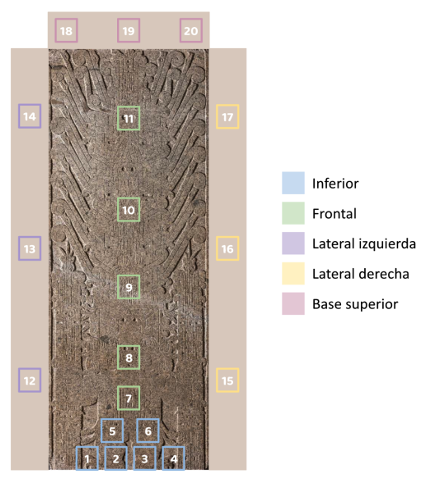
\includegraphics[width=0.8\textwidth]{images/Muestras.png}
    \caption{Esquema de muestreo de la Estela de Raimondi. Se señalan los 20 puntos de hisopado distribuidos sobre las cinco regiones del monumento (base superior, cara frontal, laterales izquierda y derecha, y sección inferior). En cada punto se recolectaron dos hisopados independientes: el hisopo A, destinado a la extracción directa de ADN para secuenciación de amplicones, y el hisopo B, destinado al cultivo de la fracción viable, posteriormente secuenciado por metagenómica \textit{shotgun}. Tomado del informe técnico de la UPCH~\cite{tsukayama2025informe}.}
    \label{fig:muestreo}
\end{figure}

Si bien la metagenómica suele aplicarse de
forma independiente de cultivo, en el estudio del patrimonio pétreo se han documentado
también aproximaciones dependientes de cultivo acopladas a la identificación molecular por
secuenciación~\cite{suchy2024}. En consecuencia, los genomas reconstruidos representan la fracción microbiana recuperable mediante cultivo y no necesariamente las poblaciones dominantes \textit{in situ}. Esta condición se trata de forma explícita como limitación en la Fase 3.


\begin{table}[htbp]
\centering
\small
\renewcommand{\arraystretch}{1.05}
\setlength{\tabcolsep}{3pt}
\caption{Bins genómicos recuperados por muestra (previos al filtrado por dominio y calidad).}
\label{tab:bins}

\makebox[\textwidth][c]{%
\begin{tabular}{c c c c c c}
\hline
\textbf{Muestra} & \textbf{N.\textsuperscript{o} bins} & \textbf{Long. total (Mb)} & \textbf{Rango bin (Mb)} & \textbf{N50 prom. (kb)} & \textbf{\%GC prom.} \\
\hline
49 & 2  & 28.1  & 0.55--27.6  & 173 & 36.2 \\
50 & 6  & 67.3  & 0.61--53.4  & 47  & 59.5 \\
51 & 1  & 4.7   & 4.73        & 189 & 52.6 \\
52 & 5  & 18.2  & 0.42--5.3   & 37  & 61.6 \\
53 & 3  & 36.9  & 2.48--29.2  & 264 & 40.5 \\
54 & 2  & 11.6  & 4.31--7.3   & 167 & 38.7 \\
55 & 1  & 34.2  & 34.24       & 404 & 51.1 \\
56 & 6  & 88.4  & 0.23--49.6  & 95  & 45.6 \\
57 & 6  & 74.7  & 0.22--39.1  & 164 & 46.9 \\
58 & 3  & 46.5  & 4.77--29.6  & 418 & 48.5 \\
59 & 2  & 29.1  & 5.91--23.2  & 283 & 40.9 \\
60 & 5  & 49.6  & 2.32--25.7  & 52  & 43.5 \\
61 & 6  & 73.1  & 0.61--40.1  & 207 & 47.7 \\
62 & 5  & 45.7  & 0.23--27.9  & 128 & 39.4 \\
63 & 6  & 88.8  & 0.37--56.5  & 40  & 45.7 \\
64 & 7  & 75.5  & 0.24--29.7  & 33  & 43.4 \\
65 & 5  & 94.8  & 0.22--29.6  & 89  & 47.0 \\
66 & 0  & ---   & ---         & --- & ---  \\
67 & 0  & ---   & ---         & --- & ---  \\
68 & 2  & 2.7   & 0.25--2.5   & 43  & 49.2 \\
69 & 2  & 2.7   & 0.25--2.5   & 40  & 49.1 \\
70 & 6  & 109.2 & 0.28--94.3  & 3   & 44.0 \\
71 & 12 & 126.9 & 0.26--101.9 & 6   & 47.2 \\
72 & 4  & 9.7   & 0.25--6.6   & 4   & 38.9 \\
\hline
\textbf{Total} & \textbf{97} & & & & \\
\hline
\end{tabular}%
}

\vspace{0.5em}

\begin{minipage}{0.95\textwidth}
\footnotesize
\textit{Nota.} Se dispuso de 24 librerías de secuenciación Illumina, identificadas con los códigos 49 a 72. El procesamiento previo, documentado por el centro de secuenciación, comprendió el ensamblaje por muestra mediante MEGAHIT, la segmentación del ensamblaje en bins genómicos mediante MetaBAT2, la evaluación de métricas de ensamblaje con QUAST y la anotación preliminar de cada bin con Bakta, junto con una asignación taxonómica preliminar basada en Kraken2. Un bin corresponde, en este punto del flujo, a un subconjunto de contigs del ensamblaje agrupados según su perfil de cobertura y composición de tetranucleótidos, bajo el supuesto de que los contigs pertenecientes a un mismo organismo comparten estas señales. Por tanto, cada bin constituye una reconstrucción parcial o completa de un genoma individual, cuya pureza taxonómica y calidad genómica se evalúan posteriormente. De las 24 librerías, 22 produjeron bins, con un total de 97 bins; las muestras 66 y 67 no recuperaron bins y fueron excluidas del análisis genómico. Las cifras mostradas corresponden a bins crudos entregados por el centro de secuenciación y preceden al filtrado por dominio y al control de calidad genómica descritos en la Fase 1; por ello, no implican que la totalidad de los bins listados sean genomas procariotas completos o libres de contaminación.
\end{minipage}

\end{table}
Las lecturas crudas (archivos FASTQ) no estuvieron disponibles para este
trabajo. Por ello, todo el flujo se ejecuta sobre los genomas ensamblados
(bins) y no sobre lecturas. En consecuencia, la importancia de cada linaje no
se mide por abundancia, sino por prevalencia espacial: el número de puntos de
muestreo distintos en los que se recuperó ese linaje. Esta métrica no depende
de las lecturas crudas y es más robusta frente al sesgo del cultivo.


\subsection{Fase 1. Control de calidad y selección de genomas (OE1)}

\subsubsection{Filtrado por dominio}

Los bins se filtraron primero por dominio para descartar contigs de origen eucariota u organelar antes de cualquier métrica basada en genes procariotas. Se utilizó Tiara \cite{karlicki2022tiara}, un clasificador de secuencias metagenómicas basado en aprendizaje profundo que opera sobre la composición de los contigs en un esquema de dos etapas. La elección de Tiara frente a Whokaryote \cite{pronk2022whokaryote} y EukRep \cite{west2018genomereconstruction} se sustentó en la matriz de selección ponderada (Tabla~\ref{tab:seleccion_software}), en la que Tiara obtuvo la mayor puntuación total gracias a su facilidad de instalación, su menor costo computacional y su capacidad adicional de identificar ADN organelar; la descripción detallada de cada herramienta evaluada se presenta en el Anexo 1.

\begin{table}[H]
\centering
\footnotesize
\caption{Matriz de selección de software para la clasificación de contigs.}
\label{tab:seleccion_software}
\begin{tabular}{@{}lcccccccc@{}}
\toprule
& & \multicolumn{2}{c}{\textbf{Tiara}} & \multicolumn{2}{c}{\textbf{Whokaryote}} & \multicolumn{2}{c}{\textbf{EukRep}} \\
\cmidrule(lr){3-4} \cmidrule(lr){5-6} \cmidrule(lr){7-8}
\textbf{Criterio} & \textbf{Peso (\%)} & \textbf{Pts} & \textbf{Peso$\times$Pts} & \textbf{Pts} & \textbf{Peso$\times$Pts} & \textbf{Pts} & \textbf{Peso$\times$Pts} \\
\midrule
Facilidad de instalación & 10 & 4 & 40 & 3 & 30 & 2 & 20 \\
Acceso a dependencias & 15 & 4 & 60 & 2 & 30 & 2 & 30 \\
Costo computacional & 10 & 3 & 30 & 2 & 20 & 3 & 30 \\
Integración en pipeline & 15 & 4 & 60 & 3 & 45 & 2 & 30 \\
Calidad de resultado & 30 & 4 & 120 & 3 & 90 & 2 & 60 \\
Alcance funcional & 10 & 4 & 40 & 2 & 20 & 2 & 20 \\
Interpretabilidad & 10 & 3 & 30 & 4 & 40 & 2 & 20 \\
\midrule
\textbf{Total} & \textbf{100} & & \textbf{380} & & \textbf{275} & & \textbf{210} \\
\bottomrule
\end{tabular}
\end{table}

Se aplicó una longitud mínima de contig de 3000 pares de bases, valor por debajo del cual los clasificadores basados en composición de secuencia pierden exactitud, y se descartaron los bins cuya fracción mayoritaria de longitud se clasificó como eucariota u organelar. Dado que Tiara discrimina entre procariotas y eucariotas pero no separa bacterias de arqueas, esta última distinción se resolvió en las fases posteriores mediante CheckM2 y GTDB-Tk.


\subsubsection{Evaluación de la calidad genómica}

La completitud y la contaminación de los bins procariotas se estimaron con CheckM2 \cite{checkm2}, que predice ambas métricas mediante modelos de aprendizaje automático entrenados sobre genomas de referencia y no requiere asignación taxonómica previa, lo que mejora su desempeño en linajes divergentes \cite{checkm2}. Se conservaron únicamente los genomas con completitud superior al 70\% y contaminación inferior al 5\%.

El umbral no corresponde a ninguna categoría MIMAG estándar. Se adoptó un valor intermedio que flexibiliza la exigencia de completitud, con el fin de recuperar genomas ambientales fragmentados, pero mantiene la restricción más estricta de contaminación (inferior al 5\%) para evitar que la posterior reconstrucción del genoma accesorio se sesgue por la inclusión de ADN foráneo \cite{bowers2017}. Este compromiso se documenta como criterio propio del proyecto y no como un estándar MIMAG de alta calidad.

\subsection{Fase 2. Asignación taxonómica y definición de linajes (OE2)}

\subsubsection{Clasificación taxonómica genómica}

Los genomas que superaron el control de calidad se clasificaron taxonómicamente con GTDB-Tk \cite{gtdbtk2019}, empleando los conjuntos de marcadores bac120 para bacterias y arc122 para arqueas. GTDB-Tk ubica cada genoma en el árbol de referencia del GTDB, que normaliza los rangos taxonómicos según la divergencia evolutiva relativa \cite{gtdbtk2019, gtdb2022}. Este enfoque basado en el genoma completo reemplaza a la asignación preliminar por Kraken2, de naturaleza basada en lecturas, por una clasificación de mayor resolución y consistencia filogenética.

\subsubsection{Confirmación de especie por ANI}

La clasificación de GTDB-Tk asigna taxonomía comparando características genómicas globales, pero no compara directamente el genoma completo contra una cepa de referencia. Para confirmar la identidad a nivel de especie, se calculó la Identidad Nucleotídica Promedio (ANI) entre cada genoma ensamblado y el genoma de referencia oficial de su taxón asignado. Este genoma de referencia corresponde a la cepa tipo de la especie (el organismo depositado en bases de datos públicas cuando esa especie fue descrita por primera vez, y que actualmente actúa como estándar de comparación).

El ANI mide qué tan parecidas son dos secuencias de ADN a lo largo del genoma completo. Dos genomas se consideran de la misma especie cuando el ANI es igual o superior al 95\% y al menos el 65\% del genoma puede alinearse \cite{fastANI2018, gtdbtk2019}.

\subsubsection{Desreplicación y definición de linajes}

Dado que el ensamblaje y el binning se realizaron por muestra de forma independiente, un mismo organismo presente en varias muestras pudo recuperarse como bins redundantes. Para colapsar esta redundancia se aplicó dRep  \cite{olm2017}, que agrupa los genomas en clústeres según su Identidad Nucleotídica Promedio (ANI). Se utilizó un umbral primario del 95\% de ANI para delimitar clústeres a nivel de especie, congruente con el radio de circunscripción taxonómica estándar empleado por la base de datos GTDB \cite{gtdbtk2019}. De forma complementaria, el agrupamiento secundario se definió a un umbral estricto del 99\% de ANI para lograr una resolución de cepa. Este último umbral permite agrupar genomas casi idénticos \cite{olm2017}, asegurando la desreplicación de poblaciones clonales sin colapsar cepas de la misma especie que pudieran albergar variaciones intraespecíficas relevantes. Cada clúster resultante se define operativamente como un linaje.

La desreplicación cumple dos funciones determinantes. Primero, provee varios genomas de la Estela por linaje, lo que habilita la construcción de un pangenoma interno con réplicas reales en la Fase 4. Segundo, permite definir una métrica de prevalencia objetiva, calculada como el número de muestras, sobre el total de 24, que aportan al menos un genoma a cada clúster. Esta métrica no depende de las lecturas crudas y por ello constituye el criterio primario de importancia de un linaje.

\subsubsection{Confirmación filogenómica}

La ubicación de cada linaje se visualizó mediante un árbol filogenómico focalizado que incluyó los genomas de la Estela y los genomas de referencia, inferido de novo por GTDB-Tk \cite{gtdbtk2019} a partir de los mismos marcadores bac120 empleados en la clasificación taxonómica. Esta elección, frente a la alternativa de inferir el árbol externamente con IQ-TREE \cite{minh2020}, se sustentó en la matriz de selección ponderada (Tabla~\ref{tab:seleccion_filogenomica}), en la que GTDB-Tk obtuvo la mayor puntuación gracias a su integración directa en el flujo ya ejecutado y a su menor costo computacional, criterio priorizado dada la restricción de cómputo propia de un proyecto de pregrado. Como contrapartida, el árbol de novo de GTDB-Tk no provee selección de modelo de sustitución ni soporte de rama mediante bootstrap, por lo que la topología resultante se interpreta como una verificación visual de la monofilia de cada linaje frente a las referencias, y no como una confirmación con soporte estadístico cuantificado.

\begin{table}[H]
\centering

\caption{Matriz de selección de software para la confirmación filogenómica.}
\label{tab:seleccion_filogenomica}

\resizebox{\textwidth}{!}{
\begin{tabular}{@{}lcccccc@{}}
\toprule
& & \multicolumn{2}{c}{\textbf{GTDB-Tk (árbol de novo)}} & \multicolumn{2}{c}{\textbf{IQ-TREE}} \\
\cmidrule(lr){3-4} \cmidrule(lr){5-6}
\textbf{Criterio} & \textbf{Peso (\%)} & \textbf{Pts} & \textbf{Peso$\times$Pts} & \textbf{Pts} & \textbf{Peso$\times$Pts} \\
\midrule
Facilidad de instalación & 20 & 4 & 80 & 3 & 60 \\
Acceso a dependencias & 20 & 4 & 80 & 3 & 60 \\
Costo computacional & 15 & 4 & 60 & 2 & 30 \\
Integración en pipeline & 20 & 4 & 80 & 3 & 60 \\
Calidad de resultado & 10 & 2 & 20 & 4 & 40 \\
Alcance funcional & 5  & 2 & 10 & 4 & 20 \\
Interpretabilidad & 10 & 2 & 20 & 4 & 40 \\
\midrule
\textbf{Total} & \textbf{100} & & \textbf{350} & & \textbf{310} \\
\bottomrule
\end{tabular}
}
\end{table}

\subsubsection{Selección de linajes para el análisis comparativo}

A partir de los linajes definidos, entendidos como los clústeres de especie obtenidos al 95\% de ANI, se priorizaron los de mayor prevalencia. Por restricciones de cómputo, el análisis comparativo se concentró en los tres linajes de mayor prevalencia. Para esta selección,  no se utilizó la abundancia de secuencias, ya que los cultivos previos en laboratorio sesgan estos números. En su lugar, se utilizó el criterio de \textbf{prevalencia espacial} \cite{olm2017}. Esto consistió en seleccionar a las especies que lograron ser ensambladas en la mayor cantidad de puntos físicos distintos de la Estela Raimondi. La detección repetida de un mismo genoma a través de múltiples muestras independientes demuestra que se trata de microorganismos residentes y estables, y no de simple polvo o contaminación ambiental

Esta elección de la especie como unidad primaria de análisis resulta indispensable para el correcto funcionamiento de Panaroo, dado que el algoritmo requiere comparar un conjunto de genomas estrechamente emparentados para diferenciar con precisión los genes esenciales y conservados (genoma core) de aquellos genes ganados o perdidos como producto de la adaptación evolutiva al nicho específico (genoma accesorio). Cuando la comparación se realiza entre genomas filogenéticamente distantes, esta distinción pierde fiabilidad, pues la divergencia de secuencia entre especies no relacionadas introduce una subestimación artificial del genoma core, atribuible a limitaciones del método de detección de ortólogos y no a una reducción real del repertorio génico compartido \cite{panaroo2020}.

%\subsection{Fase 3. Validación cruzada con el perfil ambiental 16S}

%Para evaluar la relevancia ecológica de los linajes recuperados de la fracción cultivable, su composición se contrastó con el perfil taxonómico de la comunidad ambiental total. Este perfil proviene de la secuenciación de amplicones 16S rRNA del hisopo A, procesada en el informe técnico previo frente a la base de datos SILVA \cite{tsukayama2025informe}. La comparación se realizó a nivel de género: la presencia, y en particular la abundancia, de los géneros seleccionados en el perfil ambiental se interpreta como evidencia de que dichos linajes son miembros genuinos de la comunidad colonizadora y no errores del cultivo. Dado que la taxonomía de SILVA y la del GTDB no son equivalentes, los nombres de género se armonizaron entre ambos sistemas antes de la comparación. Este paso convierte la limitación impuesta por el origen cultivado de la muestra en un control de relevancia ecológica.

\subsection{Fase 3. Análisis pangenómico comparativo (OE3)}

\subsubsection{Recopilación de genomas de referencia}

Para cada uno de los tres linajes seleccionados se recopilaron genomas de referencia desde NCBI RefSeq y GTDB. Se incluyeron genomas de la especie asignada por GTDB-Tk y, cuando el número de referencias a nivel de especie fue insuficiente, se amplió al género correspondiente. Se priorizaron los ensamblajes designados como completos o representativos en RefSeq, que ya han pasado por el proceso de curación de NCBI. Cuando un linaje no contó con referencias de especie en RefSeq, se recurrió a los genomas tipo de GTDB como alternativa.

El conjunto de referencias se desreplicó con dRep a un umbral del 99\% de ANI, con el fin de evitar que genomas casi clonales, frecuentes en taxones muy secuenciados, inflaran artificialmente el genoma núcleo. El número de genomas de referencia no se fijó de forma arbitraria, sino que se determinó mediante la curva de acumulación del pangenoma: se añadieron genomas secuencialmente hasta observar la estabilización del genoma núcleo \cite{tettelin2005}. Cuando un taxón presentó menos de aproximadamente diez genomas de referencia de calidad suficiente en bases de datos públicas, el conjunto se amplió siguiendo el mismo criterio. En el caso de los linajes arqueales, para los que la disponibilidad de referencias de calidad fue menor, el linaje se incluyó en el análisis comparativo solo si reunió genomas suficientes para estabilizar la curva; en caso contrario, se describió de forma individual sin pangenoma comparativo.

\subsubsection{Anotación estructural y funcional consistente}

La totalidad de los genomas, tanto los MAGs de la Estela como las referencias, se anotó con la misma herramienta y versión para garantizar la homogeneidad requerida por el análisis pangenómico \cite{panaroo2020}. Se empleó Bakta \cite{schwengers2021}, que realiza la predicción de marcos abiertos de lectura y la anotación mediante identificación de secuencias sin alineamiento, y que ya se había aplicado a los bins originales. Esta elección, frente a la alternativa de Prokka \cite{prokka2014} (heredero directo de Prodigal \cite{Hyatt2010}), se sustentó en la matriz de selección ponderada (Tabla~\ref{tab:seleccion_anotacion}), en la que Bakta obtuvo la mayor puntuación gracias a su continuidad con la anotación ya aplicada a los bins originales, su mayor resolución en linajes ambientales divergentes y su alcance funcional más amplio; Prokka resultó más liviano de instalar, pero con menor calidad de resultado en MAGs poco representados en bases de datos curadas. La anotación consistente evita que diferencias en la predicción génica se confundan con diferencias biológicas.

\begin{table}[H]
\centering
\footnotesize
\caption{Matriz de selección de software para la anotación estructural y funcional.}
\label{tab:seleccion_anotacion}
\begin{tabular}{@{}lcccccc@{}}
\toprule
& & \multicolumn{2}{c}{\textbf{Bakta}} & \multicolumn{2}{c}{\textbf{Prokka}} \\
\cmidrule(lr){3-4} \cmidrule(lr){5-6}
\textbf{Criterio} & \textbf{Peso (\%)} & \textbf{Pts} & \textbf{Peso$\times$Pts} & \textbf{Pts} & \textbf{Peso$\times$Pts} \\
\midrule
Facilidad de instalación & 10 & 3 & 30  & 4 & 40 \\
Acceso a dependencias    & 10 & 3 & 30  & 4 & 40 \\
Costo computacional      & 5  & 3 & 15  & 4 & 20 \\
Integración en pipeline  & 25 & 4 & 100 & 2 & 50 \\
Calidad de resultado     & 25 & 4 & 100 & 2 & 50 \\
Alcance funcional        & 15 & 4 & 60  & 3 & 45 \\
Interpretabilidad        & 10 & 4 & 40  & 3 & 30 \\
\midrule
\textbf{Total} & \textbf{100} & & \textbf{375} & & \textbf{275} \\
\bottomrule
\end{tabular}
\end{table}

\subsubsection{Reconstrucción del pangenoma}

El pangenoma de cada linaje se reconstruyó con Panaroo \cite{panaroo2020} en su modo estricto (clean-mode strict). Esta elección, frente a la alternativa de PPanGGOLiN \cite{ppanggolin2020}, se sustentó en la matriz de selección ponderada (Tabla~\ref{tab:seleccion_pangenoma}), en la que Panaroo obtuvo la mayor puntuación gracias a su representación gráfica del pangenoma, que corrige errores de anotación y de ensamblaje mediante la propagación del contexto genómico vecino y reduce de forma marcada la inflación artificial del genoma accesorio asociada a la fragmentación de los MAGs; PPanGGOLiN, pese a ofrecer un modelo probabilístico de partición con módulos adicionales (regiones de plasticidad genómica), no corrige esta inflación con la misma eficacia en colecciones de MAGs fragmentados.

\begin{table}[H]
\centering
\footnotesize
\caption{Matriz de selección de software para la reconstrucción del pangenoma.}
\label{tab:seleccion_pangenoma}
\begin{tabular}{@{}lcccccc@{}}
\toprule
& & \multicolumn{2}{c}{\textbf{Panaroo}} & \multicolumn{2}{c}{\textbf{PPanGGOLiN}} \\
\cmidrule(lr){3-4} \cmidrule(lr){5-6}
\textbf{Criterio} & \textbf{Peso (\%)} & \textbf{Pts} & \textbf{Peso$\times$Pts} & \textbf{Pts} & \textbf{Peso$\times$Pts} \\
\midrule
Facilidad de instalación & 10 & 3 & 30  & 3 & 30 \\
Acceso a dependencias    & 10 & 3 & 30  & 3 & 30 \\
Costo computacional      & 5  & 3 & 15  & 4 & 20 \\
Integración en pipeline  & 15 & 3 & 45  & 3 & 45 \\
Calidad de resultado     & 35 & 4 & 140 & 2 & 70 \\
Alcance funcional        & 15 & 3 & 45  & 4 & 60 \\
Interpretabilidad        & 10 & 4 & 40  & 3 & 30 \\
\midrule
\textbf{Total} & \textbf{100} & & \textbf{345} & & \textbf{285} \\
\bottomrule
\end{tabular}
\end{table}

El pangenoma se particionó en tres compartimentos siguiendo la convención de la genómica comparativa \cite{panaroo2020, tettelin2005, Page2015}: genoma nuclear (genes presentes en al menos el 95\% de los genomas), genoma de cubierta o shell (genes en el 15 a 95\%) y genoma accesorio o cloud (genes en menos del 15\%).

\subsubsection{Identificación de genes candidatos exclusivos de la Estela}

Los genes candidatos a ser exclusivos de la Estela se definieron como aquellos presentes en uno o más MAGs del monumento y ausentes en todos los genomas de referencia. Para reducir la probabilidad de errores, se exigió que el gen estuviera completo y no truncado en el borde de un contig. Los candidatos se contrastaron mediante búsqueda de homología frente a las bases de datos nr (non-redundant) y nt (nucleotide) para descartar contaminación. Estos genes se interpretan en el marco de la transferencia horizontal de genes como principal motor de adaptación ecológica en procariotas \cite{soucy2015}. Dado que la incompletitud de los MAGs implica que la ausencia observada de un gen no equivale a su ausencia real \cite{bowers2017}, los resultados se reportan como candidatos a exclusivos y como adquisición probable, sin afirmar certeza.

\subsection{Fase 4. Caracterización del potencial metabólico y del riesgo (OE4)}

\subsubsection{Anotación funcional del potencial metabólico}


El potencial metabólico de los linajes seleccionados se caracterizó con la herramienta DRAM \cite{dram2020}, la cual integra la asignación de ortólogos KEGG (KO) y produce resúmenes de los ciclos biogeoquímicos del nitrógeno, el azufre y el carbono, así como el inventario de enzimas activas sobre carbohidratos (CAZymes) basado en las bases dbCAN y CAZy. Para la evaluación de los módulos de KEGG, DRAM modela las vías como redes dirigidas y calcula la completitud como el porcentaje de cobertura de la ruta que presenta la mayor proporción de genes (nodos) detectados \cite{dram2020}. Sobre esta base, en el presente estudio se estableció un umbral operativo estricto: un módulo metabólico se consideró funcionalmente "presente" solo cuando su porcentaje de completitud alcanzó o superó el 66\%. Para las funciones que dependen de varios genes, la presencia se definió mediante una regla explícita para cada función, descrita en la Tabla~\ref{tab:marcadores}.

\subsubsection{Definición de marcadores de riesgo y supervivencia}

La interpretación funcional se ancló en una tabla de marcadores genómicos definida \textit{a priori}, es decir, fijada antes de observar los resultados, con el fin de evitar el sesgo de confirmación. Cada marcador corresponde a una función y no a un gen aislado, de modo que una función que requiere varios genes se cuenta una sola vez. La tabla organiza las funciones en tres categorías. La primera reúne los marcadores de riesgo de biodeterioro: la producción de ácido glucónico y de ácido 2-cetoglucónico, que acidifican el sustrato y actúan como quelantes de silicatos \cite{gutarowska2015}; la biosíntesis de sustancias poliméricas extracelulares (EPS) y la adhesión mediante curli, que sostienen la biopelícula \cite{flemming2010}; y la nitrificación y la oxidación del azufre como fuentes de ácidos inorgánicos \cite{dakal2012, zanardini2019}. La segunda reúne los marcadores de supervivencia o persistencia: la esporulación \cite{Galperin2022}, la síntesis de carotenoides, la respuesta al estrés oxidativo, la síntesis de los solutos compatibles ectoína y trehalosa, que protegen frente a la desecación, y la reparación del ADN dañado por radiación ultravioleta. La tercera reúne funciones de contexto que se reportan pero no se interpretan como marcadores de riesgo: el ciclo de los ácidos tricarboxílicos, presente en prácticamente todas las bacterias aerobias \cite{zanardini2019}, las enzimas activas sobre carbohidratos (CAZymes) \cite{cantarel2009,zhang2018} y la ureólisis, cuya precipitación de carbonato puede tanto proteger como alterar la superficie pétrea.

La Tabla~\ref{tab:marcadores} detalla, para cada función, los genes representativos, sus identificadores KEGG Orthology (KO) y la regla con la que se considera presente. Las reglas exigen los genes necesarios para que la función sea operativa. Por ejemplo, la glucosa deshidrogenasa \textit{gcd} solo se cuenta como productora de ácido glucónico si el genoma porta además los genes de síntesis de su cofactor, la pirroloquinolina quinona (\textit{pqqA}--\textit{E}). Del mismo modo, la nitrificación y la oxidación del azufre se evalúan con los módulos KEGG completos (M00528 y M00595) y no con genes aislados. Los genes cuya función no distingue el proceso de interés se excluyeron: la nitrato reductasa \textit{narG} comparte identificador KO con la nitrito oxidorreductasa \textit{nxrA}, y la sulfito reductasa disimilatoria \textit{dsrAB} participa tanto en la reducción como en la oxidación del azufre. Los identificadores KO y los módulos se verificaron directamente contra la base de datos KEGG \cite{kegg2023}. Las CAZymes no poseen un identificador KO único; su detección se realiza mediante la base de datos dbCAN, integrada en DRAM. La detección efectiva de cada función en los genomas se obtiene de DRAM durante la fase de anotación funcional.

\subsubsection{Integración del potencial funcional con la estructura del pangenoma}

En el paso final, cada marcador de la tabla \textit{a priori} se mapeó sobre la partición del pangenoma para determinar si reside en el genoma nuclear o en el accesorio. Para evaluar de forma cuantitativa si los marcadores de riesgo se concentran en el genoma accesorio, se aplicó una prueba exacta de Fisher sobre una tabla de contingencia de dos por dos que cruza la condición de gen de riesgo o no de riesgo con su pertenencia al genoma accesorio o nuclear, reportando tanto el valor de probabilidad como la razón de momios (odds ratio) como medida del tamaño del efecto. Cuando se evaluaron varias categorías funcionales de forma simultánea, los valores de probabilidad se ajustaron por comparaciones múltiples mediante el procedimiento de Benjamini y Hochberg. Esta prueba se interpreta con cautela por dos razones: las familias génicas no constituyen observaciones estadísticamente independientes, debido a la no independencia filogenética, y el número reducido de marcadores de riesgo limita la potencia estadística. Por ello, el resultado se presenta como evidencia de apoyo y no como prueba concluyente. De forma complementaria, se caracterizó la apertura del pangenoma estimando el parámetro de la ley de Heaps \cite{ppanggolin2020}.

La lógica interpretativa es la siguiente. Si los genes de biodeterioro se enriquecen de forma significativa en el genoma accesorio, en particular si son compartidos por varios MAGs del mismo linaje, ello aporta soporte cuantitativo a la hipótesis de que dichas funciones fueron adquiridas como adaptación al nicho del monumento. Si, por el contrario, residen en el genoma nuclear, se interpretan como rasgos intrínsecos y conservados del linaje. En coherencia con el alcance del estudio, estas conclusiones describen el potencial metabólico codificado y no la actividad biológica real en el momento del muestreo.

% Requiere en el preambulo: \usepackage{tabularx}
% Si el documento es a dos columnas (p. ej. IEEEtran) y la tabla queda muy
% apretada, cambia \begin{table} por \begin{table*} para que ocupe el ancho
% completo de la pagina.
\newcolumntype{Q}[1]{>{\hsize=#1\hsize\raggedright\arraybackslash}X}
\begin{table*}[htbp]
\centering
\footnotesize
\setlength{\tabcolsep}{4pt}
\caption{Marcadores genómicos \textit{a priori} de biodeterioro, supervivencia y contexto, con la regla de presencia de cada función.}
\label{tab:marcadores}
% Fuente de trabajo: metadata/marcadores_fase4.tsv del repositorio del pipeline.
% KO y modulos verificados contra la API de KEGG (rest.kegg.jp) el 06-10-2026.
\begin{tabularx}{\linewidth}{Q{0.9} Q{1.1} Q{0.9} Q{1.3} Q{1.1} Q{0.7}}
\hline
\textbf{Categoría} & \textbf{Función / mecanismo} & \textbf{Genes} & \textbf{KO} & \textbf{Regla de presencia} & \textbf{Fuente} \\
\hline
Riesgo & Ácido glucónico (acidólisis y quelación) & gcd; pqqA--E & K00117; K06135--K06139 & gcd y al menos 3 de 5 genes pqq & \cite{gutarowska2015} \\
Riesgo & Ácido 2-cetoglucónico (quelación de silicatos) & gcd; pqqA--E; gluconato 2-deshidrogenasa & K00117; K06135--K06139; K06150, K06151, K06152 & regla anterior y al menos 2 de 3 subunidades & \cite{gutarowska2015} \\
Riesgo & EPS de biopelícula (Gram positivas) & epsA--O; tasA, tapA & K19419--K19431; K06336, K19433 & al menos 66\% del operón eps, o tasA y tapA & \cite{flemming2010} \\
Riesgo & EPS de biopelícula (Gram negativas) & pgaA, pgaB, pgaC, pgaD & K11935, K11931, K11936, K11937 & al menos 3 de 4 & \cite{flemming2010} \\
Riesgo & Adhesión (curli) & csgA, csgB & K04334, K04335 & ambos & \cite{flemming2010} \\
Riesgo & Nitrificación (ácido nítrico) & amoA, amoB, amoC, hao & K28504, K10945, K10946, K10535 & módulo M00528 al 66\% (3 de 4) & \cite{zanardini2019, dram2020} \\
Riesgo & Oxidación de azufre (ácido sulfúrico) & soxA, soxX, soxY, soxZ, soxB, soxC, soxD & K17222--K17227, K22622 & módulo M00595 al 66\% (5 de 7) & \cite{zanardini2019} \\
\hline
Supervivencia & Esporulación (latencia y resistencia) & spo0A, spoIIAA, spoIIE & K07699, K06378, K06382 & al menos 2 de 3 & \cite{Galperin2022} \\
Supervivencia & Carotenoides (protección UV) & crtB, crtI & K02291 o K17841; K10027 o K15745 & módulo M00097: crtB y crtI & \cite{basile2025} \\
Supervivencia & Estrés oxidativo & katA, sodA, dps & K03781, K04564, K04047 & al menos 2 de 3 & \cite{alonso2025, basile2025} \\
% TODO: verificar que alonso2025 y basile2025 respaldan ectoina, trehalosa y fotoliasas, o agregar fuentes especificas.
Supervivencia & Desecación: ectoína & ectA, ectB, ectC & K06718, K00836, K06720 & al menos 2 de 3 & \cite{alonso2025, basile2025} \\
Supervivencia & Desecación: trehalosa & otsA, otsB & K00697, K01087 & ambos & \cite{alonso2025, basile2025} \\
Supervivencia & Reparación del daño UV & fotoliasas (phr) & K01669, K06876 & al menos 1 & \cite{basile2025} \\
\hline
Contexto & Ácidos orgánicos del ciclo TCA & gltA, acnA, icd, sdhA, fumA & K01647, K01681, K00031, K00239, K01676 & módulo M00009 (descriptivo) & \cite{zanardini2019, gutarowska2015} \\
Contexto & CAZymes (polisacáridos) & familias GH, GT & sin KO único (dbCAN) & conteo por familia (descriptivo) & \cite{cantarel2009, zhang2018} \\
% TODO: agregar una fuente para la ureolisis y la precipitacion de carbonato.
Contexto & Ureólisis (precipitación de carbonato) & ureA, ureB, ureC & K01430, K01429, K01428 & los tres (descriptivo) & --- \\
\hline
\end{tabularx}
\end{table*}


\subsection{Reproducibilidad}
Se registró la versión exacta de cada herramienta bioinformática y la versión de cada base de datos empleada, y cada identificador KO se verificó contra la versión vigente de KEGG. El conjunto de software comprende, en orden de ejecución, Tiara \cite{karlicki2022tiara}, CheckM2 \cite{checkm2}, GTDB-Tk \cite{gtdbtk2019}, FastANI \cite{fastANI2018}, dRep \cite{olm2017}, Bakta \cite{schwengers2021}, Panaroo \cite{panaroo2020} y DRAM \cite{dram2020}. Las pruebas estadísticas se ejecutaron en un entorno de R con las bibliotecas correspondientes.

Los análisis computacionalmente intensivos se ejecutaron en el clúster de cómputo de alto rendimiento Khipu de la Universidad de Ingeniería y Tecnología (UTEC), modalidad Tesis. Este tipo de acceso permite el uso de las particiones \texttt{debug}, \texttt{debug-gpu}, \texttt{standard}, \texttt{gpu} y \texttt{big-mem}, con una asignación máxima por usuario de 32 núcleos de CPU, 98 GB de memoria RAM y 40 \textit{GPU shards}, además de un tiempo máximo de ejecución de 24 horas por trabajo computacional. La disponibilidad de esta infraestructura permitió ejecutar de manera controlada y reproducible las etapas de filtrado, evaluación de calidad, clasificación taxonómica, comparación genómica, anotación funcional y análisis pangenómico.

Para asegurar la trazabilidad del flujo de trabajo, se conservaron los comandos utilizados, los parámetros de ejecución, los archivos de entrada y salida, y los registros generados por cada herramienta. Asimismo, los resultados intermedios relevantes fueron organizados por etapa del análisis. Esta estructura permite auditar cada paso del procesamiento, repetir los análisis bajo las mismas condiciones computacionales y vincular los resultados finales con los archivos originales.



%\chapter{RESULTADOS}

% ======================================================================
% CAPITULO 5 - RESULTADOS. Secciones de Fase 1 (OE1) y Fase 2 (OE2).
% Reemplaza las lineas 13-71 de cap5-resultados.tex (desde
% \section{Fase 1...} hasta justo antes de \section{Fase 3}).
%
% Figuras requeridas en images/ (copiar desde fase1_khipu/figuras/figs/):
%   fig1_embudo_seleccion.pdf      fig2_calidad_genomica.pdf
%   fig3_arbol_filogenomico.pdf    fig4_matriz_mash.pdf
%   fig5_novedad_taxonomica.pdf    fig6_prevalencia_linajes.pdf
%   fig7_composicion_taxonomica.pdf
% ======================================================================

\section{Fase 1. Control de calidad y selección de genomas (OE1)}

La Fase 1 se ejecutó en el clúster Khipu mediante el controlador
\texttt{run\_fase1.slurm} (trabajo SLURM 49286), sobre los 97 bins genómicos
crudos procedentes de las 22 librerías Illumina que recuperaron material
ensamblable (Tabla~\ref{tab:bins}). El flujo aplicó dos filtros secuenciales e
independientes: primero una discriminación por dominio con Tiara y después una
estimación de calidad genómica con CheckM2. El orden no es intercambiable, ya
que las métricas de completitud y contaminación de CheckM2 se calculan sobre
marcadores procariotas y carecen de sentido en un ensamblaje
mayoritariamente eucariota.

\subsection{Depuración secuencial del conjunto de bins}

El filtrado por dominio descartó 31 de los 97 bins, cuya mayoría se
clasificó como eucariota u organelar. Este resultado era esperable dado el
origen de las muestras: una superficie pétrea expuesta a la intemperie acumula
material fúngico, algal y vegetal que el ensamblaje por muestra no separa del
componente procariota. Casos como \texttt{bin-1-55}, con 34.2 Mb repartidos en
247 contigs, corresponden con claridad a un genoma eucariota parcialmente
reconstruido y no a un genoma bacteriano contaminado.

Los 66 bins restantes pasaron al control de calidad genómica, donde se aplicó el
criterio definido para el OE1: completitud superior al 70\% y contaminación
inferior al 5\%. De ellos, 45 fueron rechazados y 21 seleccionados, lo que
representa una tasa de retención del 21.65\% sobre el total crudo inicial. El
motivo de los rechazos resulta informativo porque distingue dos problemas de
naturaleza distinta:

\begin{itemize}
    \item \textbf{18 bins} incumplieron únicamente el criterio de completitud
    ($\le 70\%$). Se trata de reconstrucciones parciales, atribuibles a baja
    profundidad de secuenciación o a fragmentación del ensamblaje. Los valores
    cubren todo el rango, desde reconstrucciones cercanas al umbral, como
    \texttt{bin-1-50} con 62.29\%, hasta fragmentos residuales sin utilidad
    analítica, como \texttt{bin-1-52} con 6.05\%.
    \item \textbf{20 bins} incumplieron únicamente el criterio de contaminación
    ($\ge 5\text{\%}$), lo que indica quimerismo: contigs de linajes distintos
    coagrupados por MetaBAT2 durante el \textit{binning}. La magnitud es en
    ocasiones considerable, como en \texttt{bin-1-60}, con 24.87\%.
    \item \textbf{7 bins} incumplieron ambos criterios de forma simultánea. El
    caso extremo es \texttt{bin-1-58}, con 0.00\% de completitud y 17.71\% de
    contaminación, un agrupamiento sin correspondencia con ningún genoma real.
\end{itemize}


Esta diferencia es importante para entender qué se perdió en cada caso. Los 18 bins incompletos corresponden a información que estaba presente en la muestra, pero que no pudo reconstruirse completamente durante el ensamblaje. En cambio, los 20 bins contaminados contienen fragmentos de distintos organismos que fueron agrupados incorrectamente. Este segundo problema es más crítico, porque podría afectar la reconstrucción del genoma accesorio en los análisis posteriores. Por ello, se mantuvo un límite estricto de contaminación del 5\%, mientras que el umbral de completitud se fijó en 70 \%.

\begin{figure}[H]
    \centering
    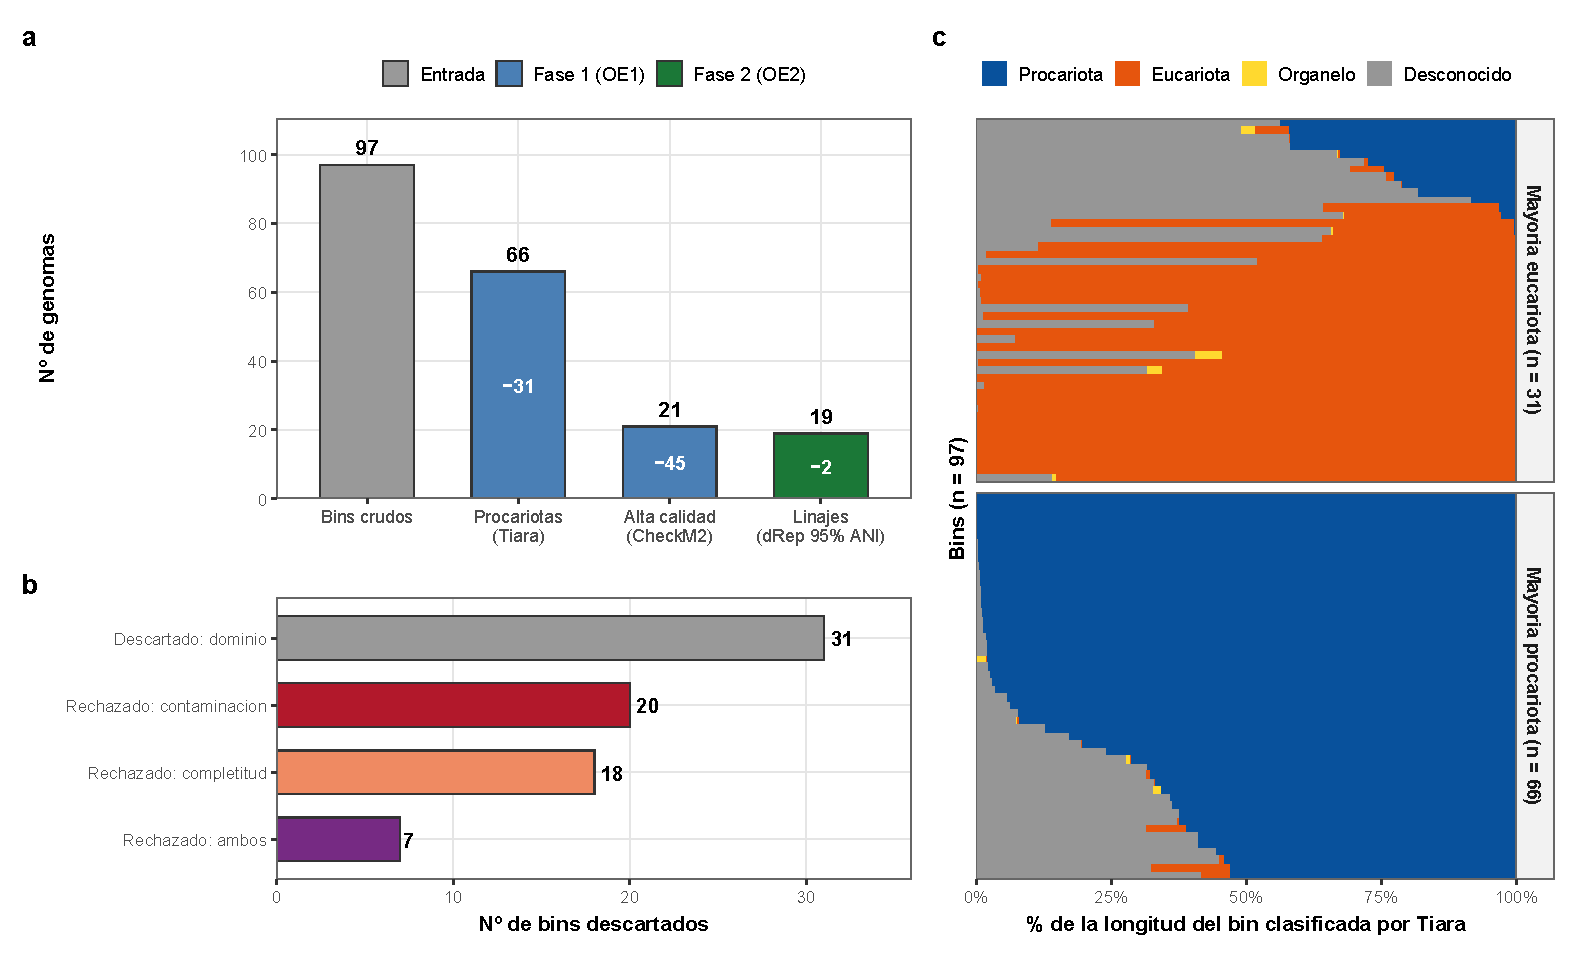
\includegraphics[width=\textwidth]{images/fig1_embudo_seleccion.pdf}
    \caption[Embudo de selección de genomas]{Embudo de selección de genomas
    desde los bins crudos hasta los linajes. \textbf{(a)} Número de genomas que
    sobrevive a cada etapa del flujo: 97 bins crudos procedentes de 22 librerías
    Illumina, 66 con dominio mayoritariamente procariota según Tiara, 21 que
    superan los umbrales de calidad de CheckM2 (completitud superior al
    70\%, contaminación inferior al 5\%) y 19 linajes tras la
    desreplicación con dRep al
    95\% de ANI. Las cifras en blanco indican las pérdidas en cada paso.
    \textbf{(b)} Motivos de descarte de los 76 bins eliminados. \textbf{(c)}
    Composición por dominio de cada uno de los 97 bins según Tiara, expresada
    como porcentaje de la longitud del bin clasificada en cada categoría; los
    bins se separan según su dominio mayoritario y se ordenan por la fracción
    procariota.}
    \label{fig:embudo}
\end{figure}

La Figura~\ref{fig:embudo}(c) muestra que la clasificación por dominio no es
ambigua en la mayoría de los casos: los bins se concentran en los extremos de
la escala, con una fracción procariota cercana al 0\% o al 100\%, y son
pocos los que ocupan posiciones intermedias. Esto respalda la decisión de
aplicar un criterio de mayoría simple sobre la longitud clasificada en lugar de
un umbral más elaborado.

\subsection{Calidad y estructura de los 21 genomas seleccionados}

Los 21 genomas retenidos presentan una calidad marcadamente asimétrica respecto
del umbral. La mediana de la completitud alcanza el 99.86\%, con 13 genomas por
encima del 99\% y 5 con completitud estimada del 100.00\%; solo cuatro
quedan por debajo del 80\%. La mediana de la contaminación es del 0.44\%, valor muy por debajo del límite fijado.

\begin{figure}[H]
    \centering
    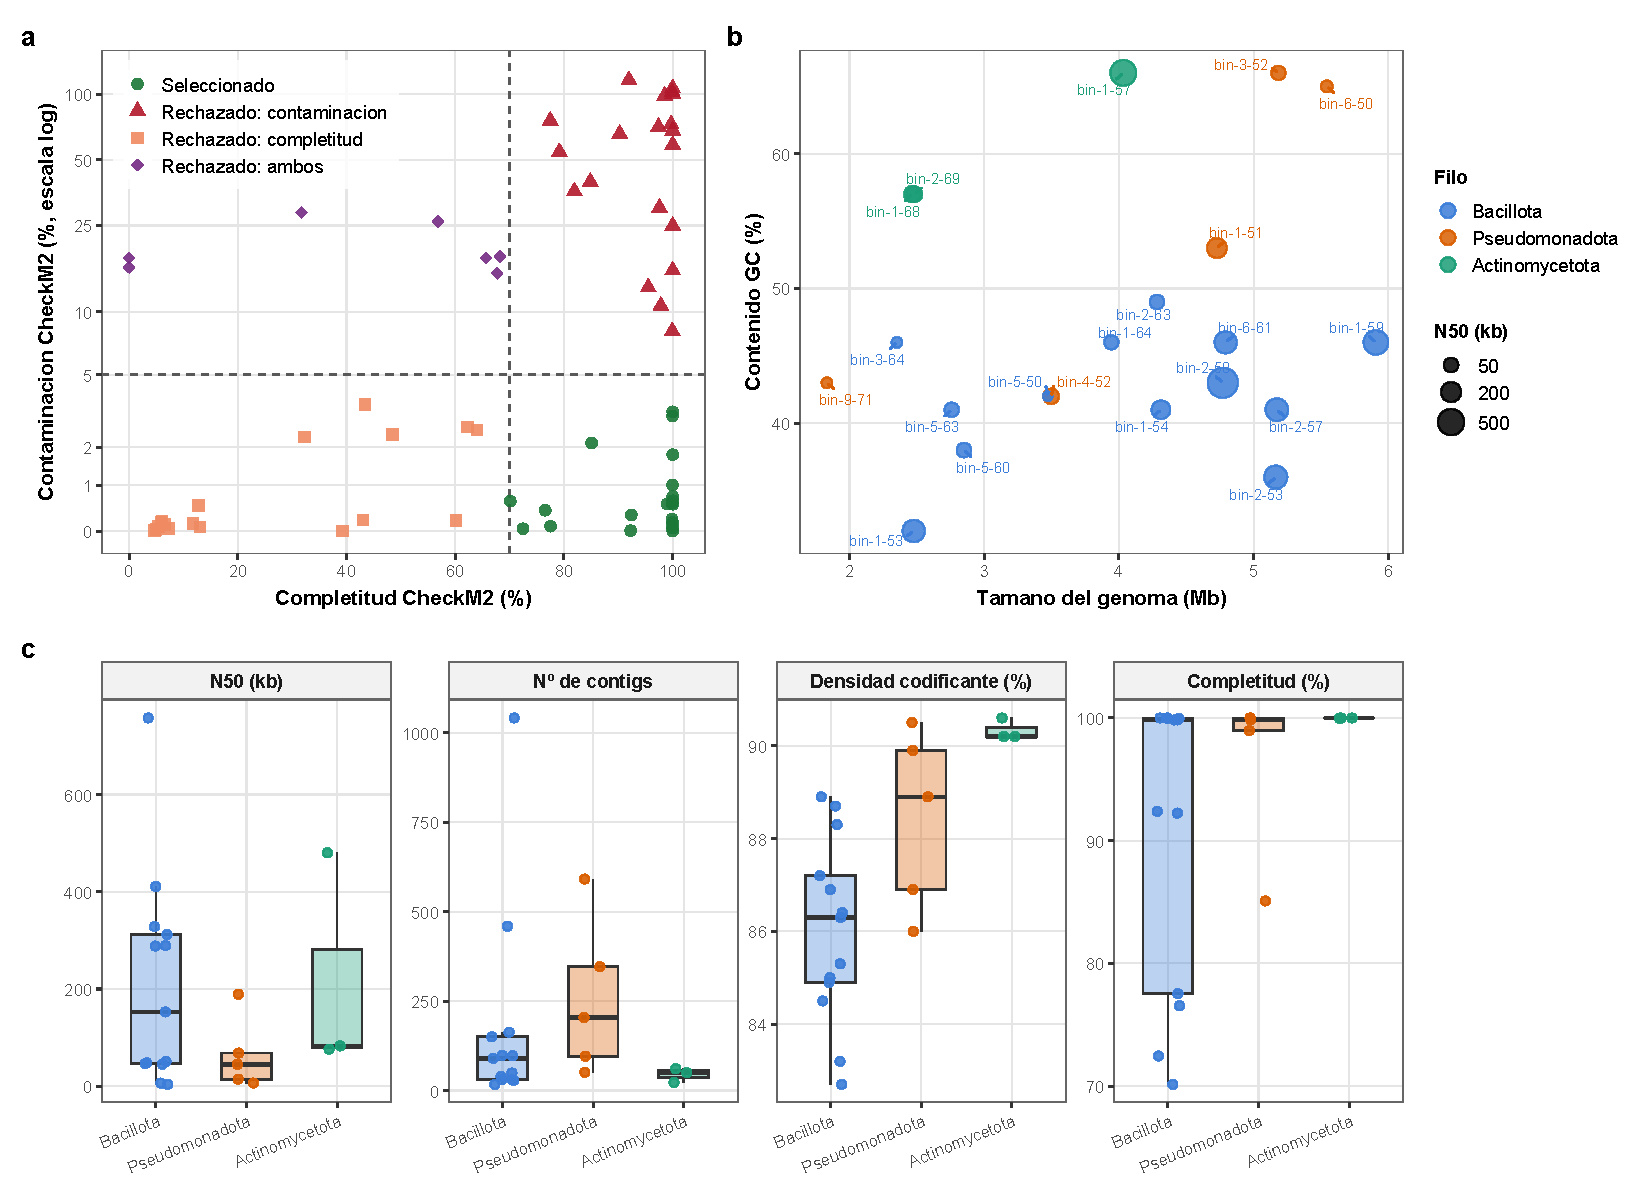
\includegraphics[width=\textwidth]{images/fig2_calidad_genomica.pdf}
    \caption[Calidad y métricas de ensamblaje]{Calidad y métricas de ensamblaje
    de los genomas. \textbf{(a)} Completitud frente a contaminación (CheckM2) de
    los 66 bins procariotas. El eje de contaminación usa escala logarítmica
    ($\log(1+x)$) porque unos pocos bins superan el 60\% y comprimirían la
    región de interés. Las líneas discontinuas marcan los umbrales del estudio
    (completitud igual o superior al 70\%, contaminación inferior al 5\%) y
    la región sombreada, los
    21 genomas seleccionados. \textbf{(b)} Tamaño del genoma frente a contenido
    GC de los 21 genomas seleccionados; el tamaño del punto es proporcional al
    N50 de los contigs y el color indica el filo. \textbf{(c)} Distribución de
    N50, número de contigs, densidad codificante y completitud por filo. Cada
    punto es un genoma; las cajas muestran mediana y cuartiles.}
    \label{fig:calidad}
\end{figure}

La Figura~\ref{fig:calidad}(a) muestra los criterios de contaminación y completitud sobre las distintas poblaciones de bins.

La completitud y la contaminación no describen por completo la utilidad de un
genoma para el análisis pangenómico. La continuidad del ensamblaje sí importa, y
en esa dimensión el conjunto es heterogéneo: el número de contigs va de 17 a
1041, con mediana de 90. Cuatro genomas superan los 300 contigs
(\texttt{bin-5-50} con 1041, \texttt{bin-6-50} con 591, \texttt{bin-3-64} con
459 y \texttt{bin-9-71} con 346).

El caso de \texttt{bin-5-50} muestra que la calidad y la fragmentación de un genoma son aspectos distintos. Este bin tiene una completitud del 76.56\% y una contaminación del 0.44\%, por lo que cumple los criterios del OE1. Sin embargo, sus 3.47 Mb están divididos en más de mil contigs, con una longitud media de solo 3.3 kb.

CheckM2 le asigna una buena calidad porque evalúa principalmente la presencia de genes marcadores, muchos de los cuales pueden encontrarse completos incluso en contigs pequeños. Por tanto, esta métrica no refleja directamente qué tan continuo está el ensamblaje.

El problema aparece en la Fase 3. Cuando un gen queda cortado entre contigs, puede no coincidir correctamente con su versión completa en los genomas de referencia. Como resultado, el análisis pangenómico puede interpretarlo como un gen diferente y clasificarlo como accesorio o incluso exclusivo de la Estela. Así, una alta fragmentación puede generar falsos genes exclusivos, afectando directamente al OE3. Por esta razón, la Fase 3 incluye controles para identificar y descartar estos casos.


Los tamaños genómicos oscilan entre 1.83 y 5.91 Mb, con mediana de 4.03 Mb,
valores compatibles con genomas bacterianos. El extremo inferior
corresponde a \texttt{bin-9-71} (1.83 Mb), cuya completitud del 85.09\%.

\begin{table}[H]
\centering
\small
\caption[Métricas de los 21 MAGs seleccionados]{Métricas de ensamblaje y calidad
genómica de los 21 MAGs seleccionados (completitud superior al 70\% y
contaminación inferior al 5\%).}
\label{tab:bins_seleccionados}
\makebox[\textwidth][c]{%
\begin{tabular}{lrrrrr}
\toprule
\textbf{Bin} & \textbf{Contigs} & \textbf{Longitud (bp)} & \textbf{Dominio} & \textbf{Completitud (\%)} & \textbf{Contaminación (\%)} \\
\midrule
bin-1-51 & 51 & 4.727.435 & prok & 100.00 & 0.00 \\
bin-1-53 & 30 & 2.476.631 & prok & 99.84 & 0.12 \\
bin-1-54 & 49 & 4.312.038 & prok & 92.25 & 0.01 \\
bin-1-57 & 22 & 4.032.412 & prok & 99.99 & 3.23 \\
bin-1-59 & 98 & 5.907.869 & prok & 99.97 & 3.07 \\
bin-1-64 & 163 & 3.944.265 & prok & 99.84 & 0.59 \\
bin-1-68 & 50 & 2.465.224 & prok & 100.00 & 1.79 \\
bin-2-53 & 39 & 5.164.804 & prok & 99.99 & 0.57 \\
bin-2-57 & 28 & 5.172.263 & prok & 99.96 & 1.01 \\
bin-2-58 & 17 & 4.771.531 & prok & 100.00 & 0.06 \\
bin-2-63 & 150 & 4.282.638 & prok & 92.39 & 0.34 \\
bin-2-69 & 61 & 2.481.071 & prok & 99.99 & 0.18 \\
bin-3-52 & 204 & 5.184.467 & prok & 98.97 & 0.58 \\
bin-3-64 & 459 & 2.352.198 & prok & 70.14 & 0.64 \\
bin-4-52 & 96 & 3.497.259 & prok & 99.86 & 0.25 \\
bin-5-50 & 1041 & 3.472.002 & prok & 76.56 & 0.44 \\
bin-5-60 & 97 & 2.849.856 & prok & 77.53 & 0.10 \\
bin-5-63 & 90 & 2.758.939 & prok & 72.46 & 0.05 \\
bin-6-50 & 591 & 5.543.214 & prok & 100.00 & 0.65 \\
bin-6-61 & 30 & 4.792.746 & prok & 100.00 & 0.74 \\
bin-9-71 & 346 & 1.832.072 & prok & 85.09 & 2.13 \\
\bottomrule
\end{tabular}%
}
\end{table}

\subsection{Implicancia para el OE1}

El OE1 se cumple. Obtenemos un conjunto de 21 genomas procariotas cuya
completitud y pureza permiten la asignación taxonómica y la comparación
genómica posteriores. Por ese motivo descartamos 78.35\% del material de
partida. La depuración  descarta
organismos que estuvieran presentes en la estela pero que no alcanzan la calidad necesaria para los posteriores análisis. Por lo tanto, la diversidad
real de la fracción viable es mayor que la que estos 21 genomas representan.

El detalle de todos los 97 bins evaluados, con los motivos específicos para su
exclusión, se presenta en el Anexo~\ref{anexo:tabla_completa_bins}.

\section{Fase 2. Asignación taxonómica y definición de linajes (OE2)}

La Fase 2 se ejecutó en Khipu mediante \texttt{run\_fase2.slurm} (trabajo SLURM
49316) sobre los 21 genomas seleccionados en la fase anterior. El flujo
comprendió la clasificación taxonómica con GTDB-Tk sobre los datos de la versión
R220, la confirmación de especie por ANI, la desreplicación en linajes con dRep
y el cálculo de la prevalencia espacial de cada linaje.

\subsection{Composición taxonómica de la fracción viable}

GTDB-Tk clasificó los 21 genomas dentro de tres filos bacterianos. No se detectó
ningún genoma arqueal, lo que resuelve la ambigüedad que
Tiara había dejado abierta en la Fase 1 entre bacterias y arqueas. La
distribución está dominada por Bacillota, con 13 genomas (62\%), seguido de
Pseudomonadota con 5 (24\%) y Actinomycetota con 3 (14\%). Por debajo del
filo, la diversidad es alta en relación con el tamaño de la muestra: los 21
genomas se reparten en 11 órdenes y 17 géneros distintos, y solo cuatro géneros
aportan más de un genoma.

\begin{figure}[H]
    \centering
    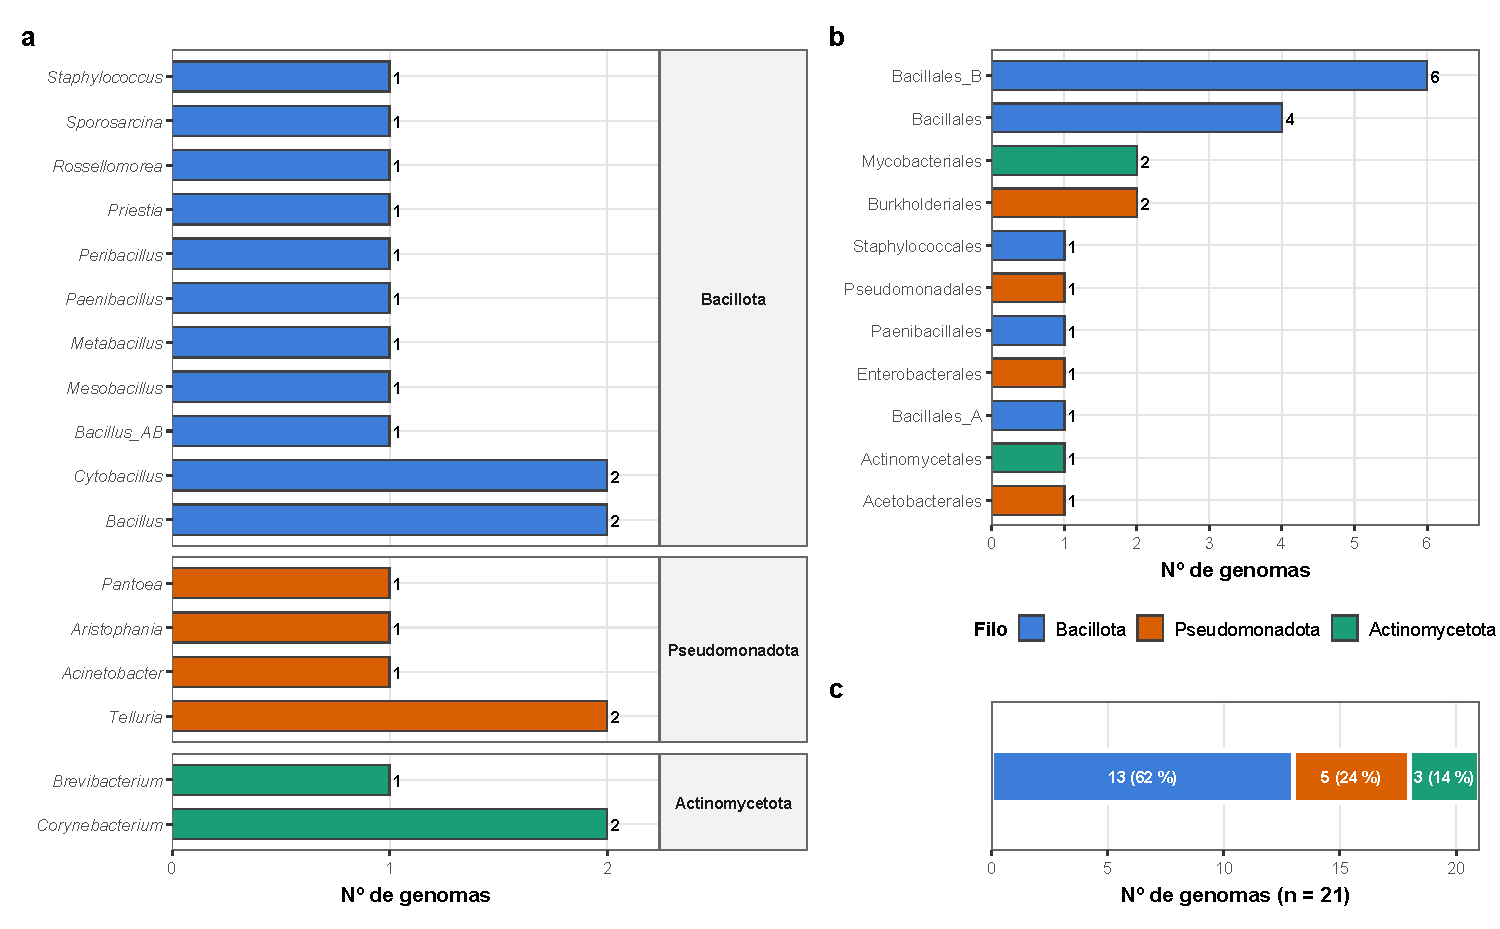
\includegraphics[width=\textwidth]{images/fig7_composicion_taxonomica.pdf}
    \caption[Composición taxonómica]{Composición taxonómica del conjunto de
    genomas seleccionados. \textbf{(a)} Número de genomas por género, agrupados
    por filo. \textbf{(b)} Número de genomas por orden. \textbf{(c)} Reparto de
    los 21 genomas entre los tres filos detectados.}
    \label{fig:composicion}
\end{figure}

El predominio de Bacillota (Figura~\ref{fig:composicion}) es coherente con el
sustrato y con el método de obtención de la muestra. Buena parte de los géneros
recuperados dentro de este filo (\textit{Bacillus}, \textit{Peribacillus},
\textit{Priestia}, \textit{Cytobacillus}, \textit{Metabacillus},
\textit{Rossellomorea}, \textit{Mesobacillus}, \textit{Sporosarcina},
\textit{Paenibacillus}) forma endosporas, una estrategia de resistencia que
favorece la supervivencia sobre una superficie pétrea expuesta a desecación,
radiación ultravioleta y oscilación térmica    \cite{jroundi2020}. 

\subsection{Confirmación filogenómica}

\begin{figure}[H]
    \centering
    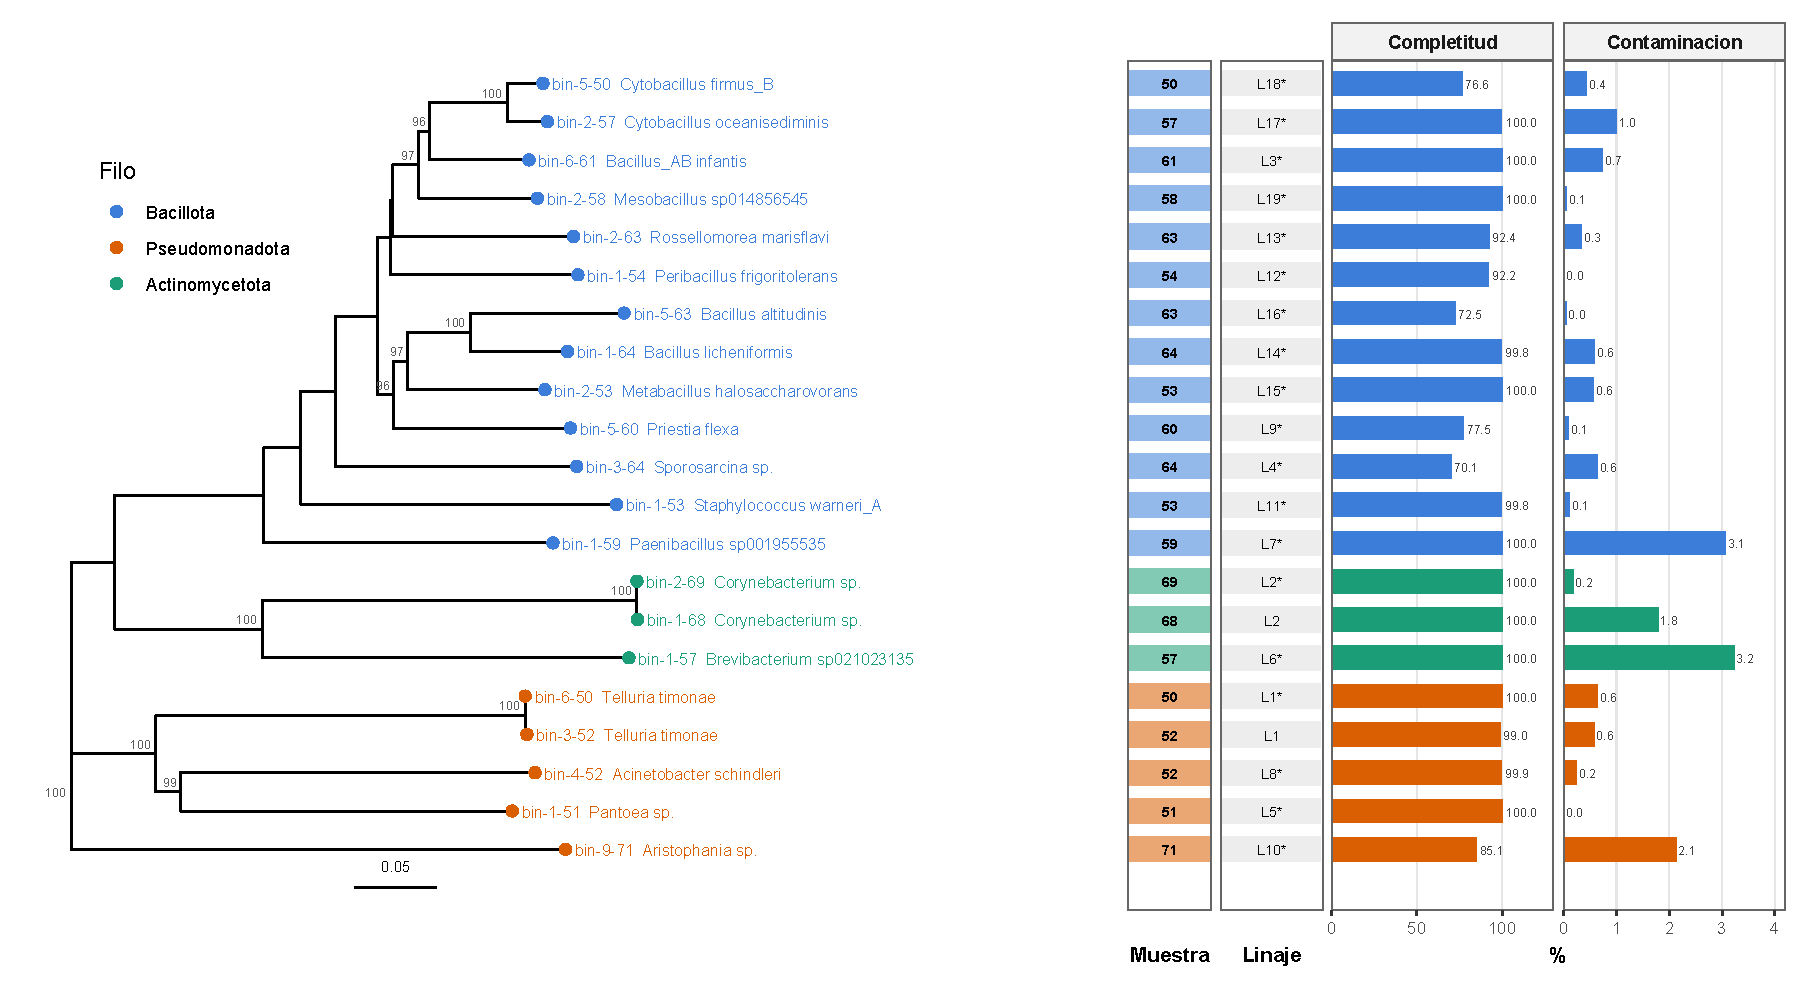
\includegraphics[width=\textwidth]{images/fig3_arbol_filogenomico.pdf}
    \caption[Árbol filogenómico de los 21 genomas]{Árbol filogenómico de los 21
    genomas seleccionados con sus metadatos. Árbol de Neighbor-Joining calculado
    sobre distancias-p a partir del alineamiento concatenado de los 120
    marcadores bacterianos de copia única (bac120, 5035 posiciones) generado por
    GTDB-Tk (datos R220), enraizado en el filo Pseudomonadota. Los números sobre
    las ramas son valores de soporte de \textit{bootstrap} (500 réplicas); solo
    se muestran los iguales o superiores al 70\%. Las columnas de la derecha
    indican, para cada
    genoma, la muestra de origen, el linaje asignado por dRep (el asterisco marca
    el genoma representante del linaje) y los valores de completitud y
    contaminación de CheckM2.}
    \label{fig:arbol}
\end{figure}

La topología del árbol (Figura~\ref{fig:arbol}) es congruente con la asignación
taxonómica: los tres filos se recuperan como grupos separados y los genomas del
mismo género quedan en ramas adyacentes. Los valores de soporte son altos en los
nodos que definen la estructura principal, con \textit{bootstrap} del 100\% en
la separación de los filos y en los pares congenéricos.

El alcance de este resultado es limitado. El árbol es de distancias y se
calculó únicamente sobre los genomas de consulta, sin incorporar genomas de
referencia de GTDB, de modo que verifica la coherencia interna del conjunto pero
no constituye una prueba filogenética independiente de la asignación taxonómica.
Tal como se justificó en el Capítulo IV, el árbol de novo focalizado por linaje,
con referencias del taxón asignado y grupo externo, queda previsto para la
Fase 4.

\subsection{Confirmación de especie y candidatos a novedad taxonómica}

Se calculó la Identidad Nucleotídica Promedio de cada genoma frente a su
referencia GTDB más próxima, aplicando los criterios de confirmación de especie
definidos en el Capítulo IV (ANI $\ge 95\%$ y fracción alineada $\ge 65\%$).
Dieciséis de los 21 genomas satisfacen ambos criterios, con valores de ANI entre
95.61\% y 99.99\% y mediana de 98.53\%. Doce de los 16 superan el 98\% de ANI, lo que indica correspondencias con especies
descritas.

\begin{figure}[H]
    \centering
    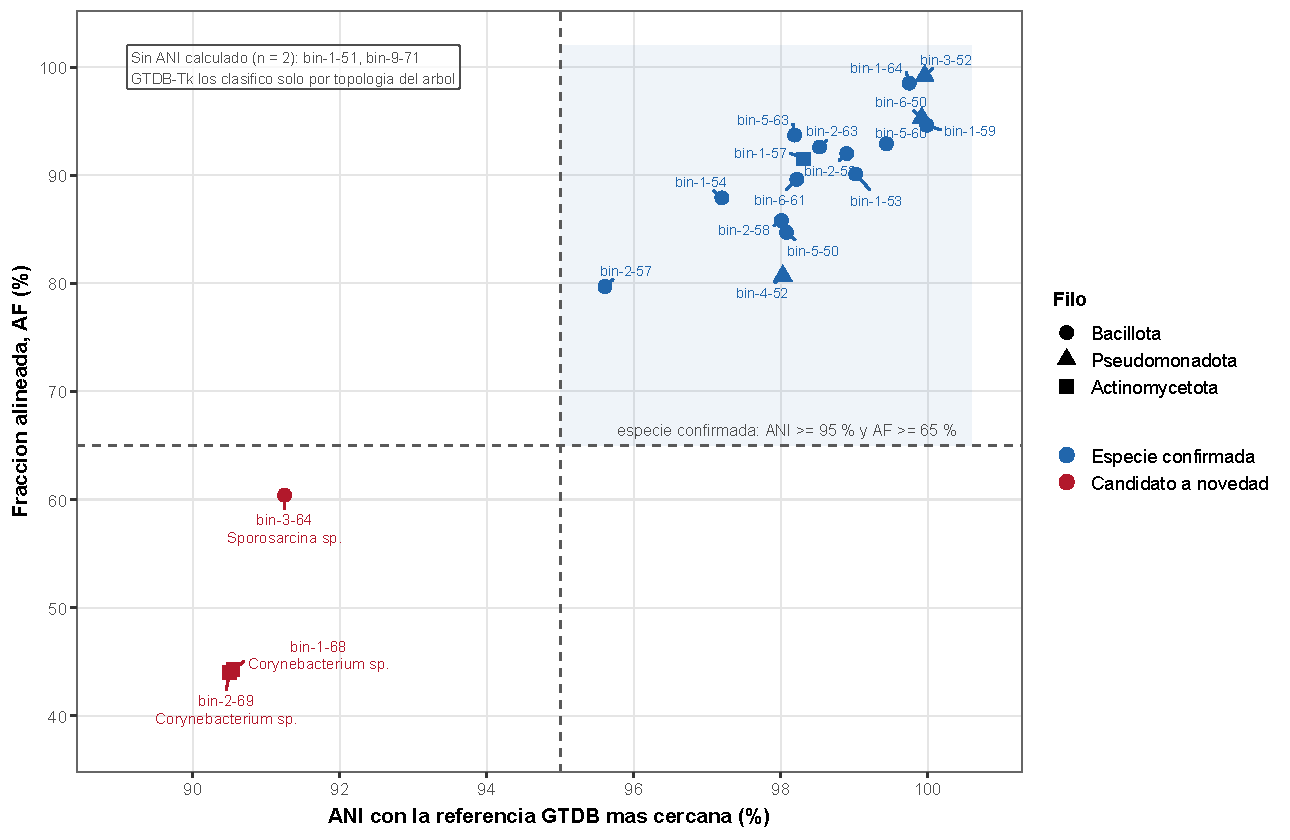
\includegraphics[width=0.85\textwidth]{images/fig5_novedad_taxonomica.pdf}
    \caption[Evaluación de novedad taxonómica]{Evaluación de novedad taxonómica
    frente a la referencia GTDB más cercana. ANI frente a fracción alineada (AF)
    de cada genoma respecto de su referencia GTDB más cercana. Las líneas
    discontinuas marcan los criterios de confirmación de especie (ANI
    igual o superior al 95\% y AF igual o superior al 65\%). Los 16 genomas
    del cuadrante sombreado
    tienen especie confirmada. Dos genomas adicionales (\texttt{bin-1-51},
    \textit{Pantoea} sp., y \texttt{bin-9-71}, \textit{Aristophania} sp.) fueron
    clasificados únicamente por topología del árbol, sin cálculo de ANI, y no
    aparecen representados.}
    \label{fig:novedad}
\end{figure}

Los 5 genomas restantes se distribuyen en dos situaciones distintas
(Figura~\ref{fig:novedad}). Dos de ellos, \texttt{bin-1-51}
(\textit{Pantoea} sp.) y \texttt{bin-9-71} (\textit{Aristophania} sp.), fueron
ubicados por GTDB-Tk mediante la topología del árbol de colocación sin que se
calculara ANI, de modo que su clasificación se detiene en el rango de género por
ausencia de una referencia suficientemente próxima. Por ese motivo, esas secuencias se descartan para la fase 3.

Los otros 3 sí produjeron valores de ANI, pero por debajo del umbral de
especie, y constituyen el hallazgo taxonómico más relevante de esta fase. Los
dos genomas de \textit{Corynebacterium} sp. (\texttt{bin-1-68} y
\texttt{bin-2-69}) alcanzan un ANI de 90.55 y 90.50\% frente a su referencia
más cercana, con fracciones alineadas de apenas 44,3 y 44.0\%. El genoma de
\textit{Sporosarcina} sp. (\texttt{bin-3-64}) queda en 91.25\% de ANI y
60.4\% de AF. Los tres valores de ANI se encuentran por debajo del umbral de similitud utilizado para la circunscripción de especies en GTDB, lo que indica que ninguno de estos genomas puede asignarse a la misma especie que su referencia más cercana. 

En el caso de los \textit{Corynebacterium}
la fracción alineada, inferior al 45\%, indica que menos de la mitad del genoma
encuentra correspondencia en la referencia. Estos genomas son, por tanto,
candidatos a especies no descritas en la versión R220 del GTDB. 

Hacemos énfasis en este resultado porque ambos \textit{Corynebacterium} proceden de muestras
distintas y presentan completitud del 100\%, de modo que la divergencia
observada no es atribuible a una reconstrucción defectuosa.

\subsection{Desreplicación y definición de linajes}

La desreplicación con dRep agrupó los 21 genomas en 19 linajes, definidos como
clústeres de especie al 95\% de ANI. Solo dos pares colapsaron.

\begin{figure}[H]
    \centering
    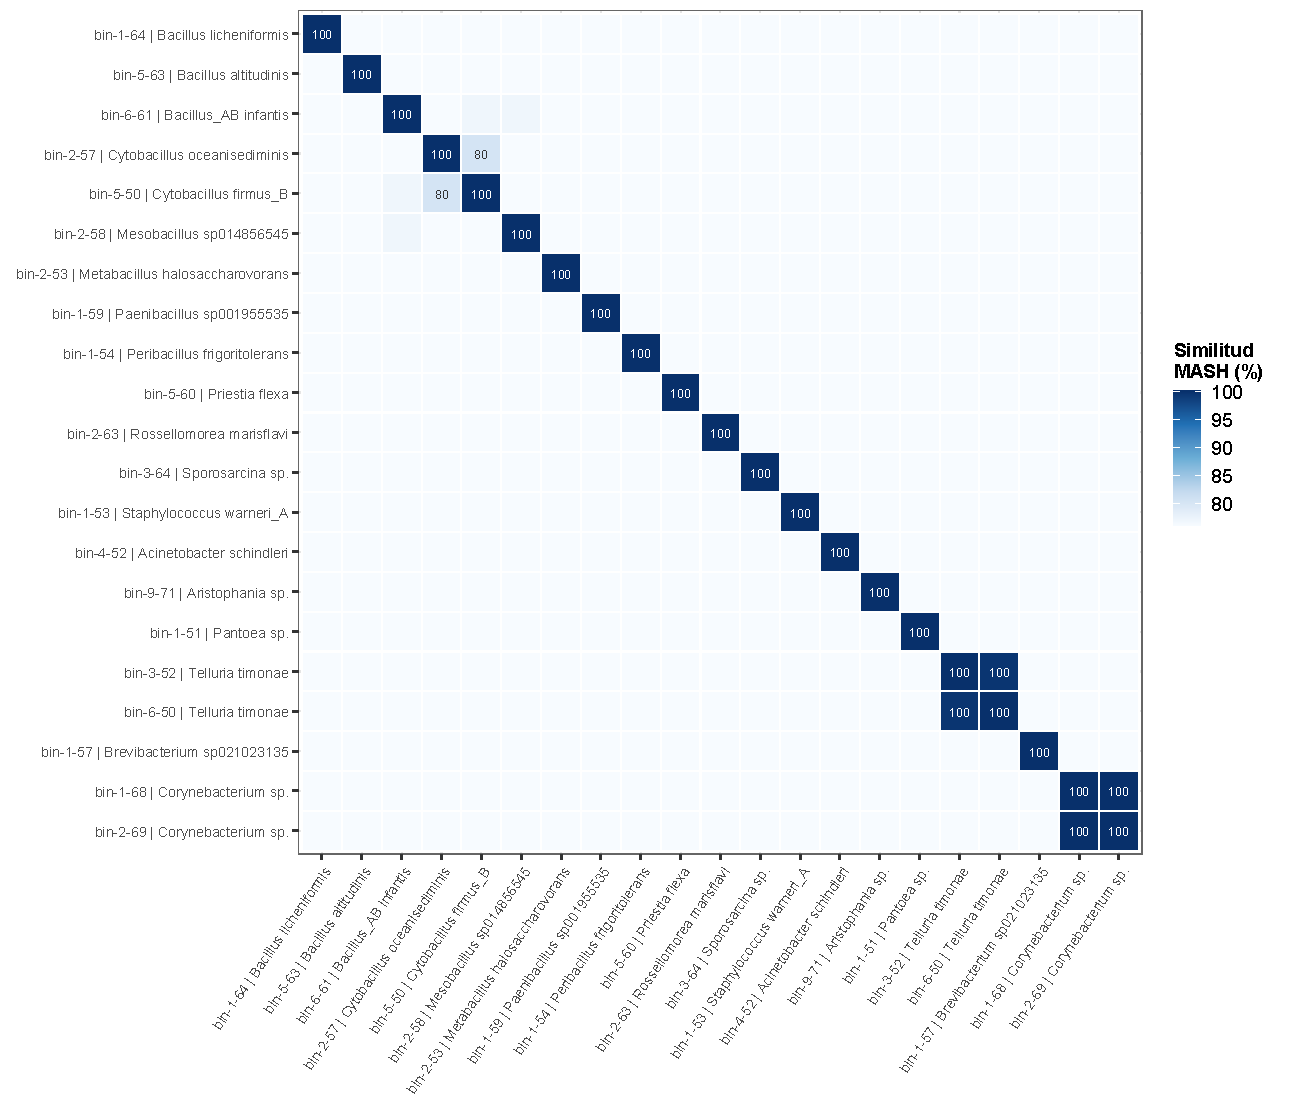
\includegraphics[width=0.9\textwidth]{images/fig4_matriz_mash.pdf}
    \caption[Matriz de similitud genómica]{Matriz de similitud genómica entre
    los 21 genomas seleccionados. Similitud MASH ($100 -$ distancia MASH) entre
    todas las parejas de genomas, ordenadas por filo y género. Solo dos parejas
    presentan similitud máxima: los dos \textit{Telluria timonae} (muestras 50 y
    52) y los dos \textit{Corynebacterium} sp. (muestras 68 y 69). Nota
    metodológica: dRep ejecuta fastANI únicamente dentro de cada clúster primario
    definido por MASH, de modo que no existe una matriz de ANI completa para los
    21 genomas; la matriz de todos contra todos disponible es la de MASH.}
    \label{fig:mash}
\end{figure}

Las dos parejas sometidas a fastANI dentro de su clúster primario superan el
umbral de especie con amplitud: \textit{Corynebacterium} sp.
(\texttt{bin-1-68} $\leftrightarrow$ \texttt{bin-2-69}) alcanza 99.96\% de ANI
con 97.1\% de cobertura del alineamiento, y \textit{Telluria timonae}
(\texttt{bin-3-52} $\leftrightarrow$ \texttt{bin-6-50}), 99.78\% de ANI con
85.2\% de cobertura. Ambas colapsan en un único linaje.

El resto de los genomas resulta mutuamente distante
(Figura~\ref{fig:mash}), incluido el par de \textit{Cytobacillus}
(\texttt{bin-5-50} y \texttt{bin-2-57}), que pese a compartir género se mantiene
como dos linajes separados con una similitud MASH del 80\%. Este es el motivo
de que 21 genomas den lugar a 19 linajes y no a un número menor: la redundancia
entre muestras es baja, y la mayor parte de lo recuperado corresponde a
organismos distintos y no a reconstrucciones repetidas del mismo genoma.

\subsection{Prevalencia espacial de los linajes}

\begin{figure}[H]
    \centering
    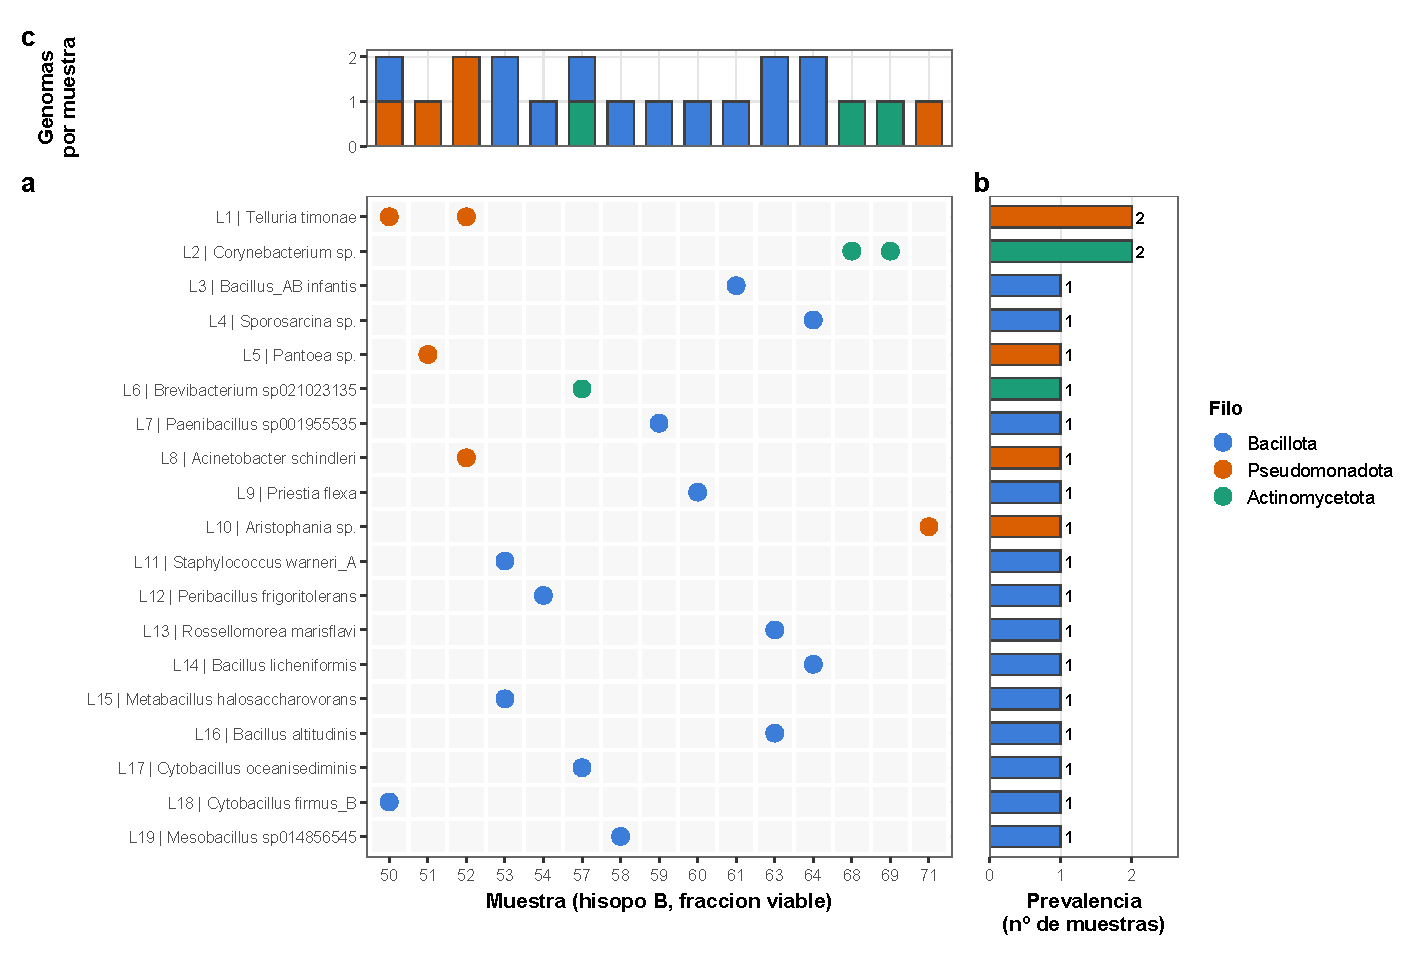
\includegraphics[width=\textwidth]{images/fig6_prevalencia_linajes.pdf}
    \caption[Prevalencia espacial de los linajes]{Prevalencia espacial de los
    linajes. \textbf{(a)} Matriz de presencia de cada linaje (filas, ordenadas
    por prevalencia descendente) en cada muestra (columnas); el color indica el
    filo. \textbf{(b)} Prevalencia de cada linaje, definida como el número de
    muestras distintas en que aparece, coloreada por filo. \textbf{(c)} Número de
    genomas de alta calidad recuperados por muestra, coloreado por filo.
    Limitación: la prevalencia se calcula sobre el número de muestras y no sobre
    zonas físicas de la estela, porque no se dispone de un mapeo
    muestra $\rightarrow$ zona en formato analizable.}
    \label{fig:prevalencia}
\end{figure}

La prevalencia espacial resultó baja en todo el conjunto. Diecisiete de los 19
linajes aparecen en una sola muestra, y solo dos alcanzan una prevalencia de
dos: L1 (\textit{Telluria timonae}, muestras 50 y 52) y L2
(\textit{Corynebacterium} sp., muestras 68 y 69). Ningún linaje se recuperó en
tres o más puntos. Además, de las 22 librerías que produjeron bins, solo 15
aportaron al menos un genoma de alta calidad tras la Fase 1
(Figura~\ref{fig:prevalencia}(c)).

Este resultado limita el poder discriminante de la métrica. Con un rango
efectivo de apenas dos valores, la prevalencia no permite ordenar los linajes ni separar con seguridad a los colonizadores
estables de las detecciones puntuales.

Dos hipotésis resultan compatibles con los datos. La primera es que la comunidad
viable de la estela sea genuinamente heterogénea entre muestras, sin un núcleo de
organismos compartido. La segunda es que la recuperación de genomas de alta calidad sea limitada, de modo que un linaje presente en varias muestras solo pueda reconstruirse con suficiente calidad en una de ellas.

Los datos disponibles no permiten discriminar entre ambas. La segunda tampoco puede descartarse, dado que el flujo retuvo apenas el 21.65\% de los bins iniciales.

Por esta razón, la prevalencia espacial se reporta aquí como caracterización de
la distribución de cada linaje sobre el monumento, pero no se emplea como
criterio para decidir qué especies ingresan al análisis pangenómico. 

Por ese motivo, el criterio de selección de bins para el pangenoma (fase 3) cambia como se explica en la siguiente sección. 

\subsection{Implicancia para el OE2}

El OE2 se cumple: los 21 genomas quedan clasificados con resolución de especie
en 16 casos y de género en los 5 restantes, y agrupados en 19 linajes
operativos que constituyen la unidad de análisis de las fases siguientes.

Dos resultados condicionan el diseño posterior. El primero es la baja
redundancia entre muestras: con 19 linajes sobre 21 genomas, y 17 de ellos
representados por un único genoma, no es posible construir un pangenoma
empleando exclusivamente material de la estela. El análisis pangenómico de la
Fase 3 debe apoyarse necesariamente en conjuntos de genomas de referencia
públicos. El segundo es la detección de tres candidatos a especies no descritas,
entre ellos los dos \textit{Corynebacterium} de completitud íntegra, que por
carecer de referencia comparable quedan fuera del análisis pangenómico pero
constituyen un hallazgo reportable por sí mismo.

\begin{table}[H]
\centering
\footnotesize
\setlength{\tabcolsep}{4pt}
\caption[Linajes definidos en la Fase 2]{Linajes definidos en la Fase 2,
ordenados por prevalencia espacial descendente.}
\label{tab:linajes}
\makebox[\textwidth][c]{%
\begin{tabular}{llrlll}
\toprule
\textbf{Linaje} & \textbf{Taxonomía (GTDB)} & \textbf{Prev.} & \textbf{Muestras} & \textbf{Representante} & \textbf{Especie conf.} \\
\midrule
L1  & \textit{Telluria timonae}              & 2 & 50, 52 & bin-6-50 & Sí \\
L2  & \textit{Corynebacterium} sp.           & 2 & 68, 69 & bin-2-69 & No \\
L3  & \textit{Bacillus\_AB infantis}         & 1 & 61 & bin-6-61 & Sí \\
L4  & \textit{Sporosarcina} sp.              & 1 & 64 & bin-3-64 & No \\
L5  & \textit{Pantoea} sp.                   & 1 & 51 & bin-1-51 & --- \\
L6  & \textit{Brevibacterium} sp021023135    & 1 & 57 & bin-1-57 & Sí \\
L7  & \textit{Paenibacillus} sp001955535     & 1 & 59 & bin-1-59 & Sí \\
L8  & \textit{Acinetobacter schindleri}      & 1 & 52 & bin-4-52 & Sí \\
L9  & \textit{Priestia flexa}                & 1 & 60 & bin-5-60 & Sí \\
L10 & \textit{Aristophania} sp.              & 1 & 71 & bin-9-71 & --- \\
L11 & \textit{Staphylococcus warneri\_A}     & 1 & 53 & bin-1-53 & Sí \\
L12 & \textit{Peribacillus frigoritolerans}  & 1 & 54 & bin-1-54 & Sí \\
L13 & \textit{Rossellomorea marisflavi}      & 1 & 63 & bin-2-63 & Sí \\
L14 & \textit{Bacillus licheniformis}        & 1 & 64 & bin-1-64 & Sí \\
L15 & \textit{Metabacillus halosaccharovorans} & 1 & 53 & bin-2-53 & Sí \\
L16 & \textit{Bacillus altitudinis}          & 1 & 63 & bin-5-63 & Sí \\
L17 & \textit{Cytobacillus oceanisediminis}  & 1 & 57 & bin-2-57 & Sí \\
L18 & \textit{Cytobacillus firmus\_B}        & 1 & 50 & bin-5-50 & Sí \\
L19 & \textit{Mesobacillus} sp014856545      & 1 & 58 & bin-2-58 & Sí \\
\bottomrule
\end{tabular}%
}

\vspace{0.5em}
\begin{minipage}{0.95\textwidth}
\footnotesize
\textit{Nota.} Prev.: prevalencia espacial, número de muestras distintas que
aportan al menos un genoma al linaje. Especie conf.: confirmación de especie por
ANI igual o superior al 95\% y AF igual o superior al 65\%; el guion indica
los linajes clasificados por
topología del árbol, sin cálculo de ANI. Los sufijos \texttt{\_A} y \texttt{\_B}
y los epítetos alfanuméricos del tipo \texttt{sp}$\langle$dígitos$\rangle$
corresponden a la nomenclatura propia del GTDB.
\end{minipage}
\end{table}

\chapter{DISEÑO TECNOLÓGICO}

% ======================================================================
% CAPITULO VI - DISENO TECNOLOGICO
% Alcance: Fases 1 y 2 (OE1 y OE2), que son las implementadas y ejecutadas.
%
% DELIMITACION RESPECTO DEL CAPITULO IV:
% El Capitulo IV justifica la eleccion de cada herramienta y el valor de cada
% umbral con sus matrices de seleccion ponderada y sus citas. Este capitulo NO
% repite esa justificacion: toma los umbrales como especificacion de entrada y
% documenta el dimensionamiento computacional, la seleccion de versiones y
% entornos, la implementacion en codigo y la arquitectura del sistema.
%
% PREAMBULO REQUERIDO EN main.tex (agregar junto a los demas \usepackage):
%   \usepackage{tikz}
%   (las figuras de 6.4 usan solo tikz base: no requieren \usetikzlibrary)
%   \usepackage{listings}
%   \lstset{
%     basicstyle=\ttfamily\scriptsize,
%     columns=fixed, basewidth={0.5em,0.45em}, keepspaces=true,
%     breaklines=true, breakatwhitespace=true, breakindent=0pt,
%     frame=leftline, framerule=0.8pt, framesep=8pt, xleftmargin=12pt,
%     aboveskip=1.2\baselineskip, belowskip=1.0\baselineskip,
%     abovecaptionskip=6pt, showstringspaces=false,
%     captionpos=b, tabsize=2, numbers=none}
%   \renewcommand{\lstlistingname}{Código}
% ======================================================================

Este capítulo documenta la construcción del flujo bioinformático con el que se
ejecutaron las Fases 1 y 2. El Capítulo IV estableció qué
herramientas se emplean, por qué se eligieron frente a sus alternativas y qué
valor toma cada umbral. Este capítulo parte de esas decisiones y no las repite.
Frente a ello, el objetivo de este capítulo es determinar el tamaño de los recursos que el flujo
necesita, seleccionar las versiones y los entornos que lo hacen ejecutable sobre
la infraestructura disponible, implementarlo en código y describir la
arquitectura que resulta de integrar todas sus piezas.

\section{Cálculo de los parámetros y dimensionamiento de los componentes}

El dimensionamiento del flujo bioinformático no consiste en calcular el
volumen de un equipo, sino en determinar cuántos recursos de cómputo,
almacenamiento y tiempo consume cada etapa, y comprobar que esos consumos caben
en la infraestructura disponible. Esta sección establece primero las bases de
diseño, que son el volumen de datos de entrada y los parámetros operativos
heredados del marco metodológico, y a partir de ellas dimensiona cada etapa.

\subsection{Bases de diseño: el conjunto de datos de entrada}

El sistema opera sobre genomas ya ensamblados y agrupados. No procesa lecturas crudas. Esta condición fija las características de la entrada y, con ella, el orden de magnitud de todo el
dimensionamiento posterior. La Tabla~\ref{tab:bases_diseno} resume las
características del conjunto.

\begin{table}[H]
\centering
\small
\caption[Bases de diseño del conjunto de entrada]{Características del conjunto
de bins de entrada, medidas sobre los archivos FASTA de origen.}
\label{tab:bases_diseno}
\begin{tabular}{lr}
\toprule
\textbf{Característica} & \textbf{Valor} \\
\midrule
Bins de entrada                       & 97 \\
Librerías de origen                   & 22 \\
Volumen total de secuencia            & 1.12 Gpb \\
Contigs totales                       & 151\,180 \\
Tamaño mediano por bin                & 4.28 Mpb \\
Tamaño mínimo por bin                 & 0.22 Mpb \\
Tamaño máximo por bin                 & 101.9 Mpb \\
Contigs en el bin más fragmentado     & 41\,610 \\
\bottomrule
\end{tabular}
\end{table}

Dos cifras de esta tabla condicionan el diseño. La primera es el tamaño máximo
de 101.9 Mpb, que corresponde a \texttt{bin-11-71}. Un bin de ese tamaño no es
un genoma bacteriano sino una mezcla, y su presencia en la entrada obliga a que
la primera etapa del flujo sea capaz de procesar archivos un orden de magnitud
mayores que el caso típico. La segunda es el volumen total de 1.12 Gpb, que es
modesto para los estándares de la metagenómica. El cuello de botella del sistema
no está, por tanto, en el tamaño de los datos propios, sino en el tamaño de las
bases de datos de referencia que el flujo debe consultar.

\subsection{Parámetros operativos del diseño}

Los parámetros que gobiernan cada etapa se establecieron en el Capítulo IV junto
con su fundamento. La Tabla~\ref{tab:parametros_operativos} los reúne en la
forma en que quedan codificados en el sistema, que es como variables de
configuración al inicio de cada script de ejecución. El propósito de esta tabla no es
justificarlos de nuevo, sino dejar constancia de la correspondencia exacta entre
el valor definido en la metodología y el valor implementado.

\begin{table}[H]
\centering
\small
\caption[Parámetros operativos implementados]{Parámetros operativos del diseño y
variable con que se implementan. La justificación de cada valor se encuentra en
el Capítulo IV.}
\label{tab:parametros_operativos}
\makebox[\textwidth][c]{%
\begin{tabular}{lllr}
\toprule
\textbf{Fase} & \textbf{Parámetro} & \textbf{Variable en el código} & \textbf{Valor} \\
\midrule
1 & Longitud mínima de contig      & \texttt{MIN\_CONTIG\_LEN}   & 3000 \\
1 & Completitud mínima             & \texttt{MIN\_COMPLETENESS}  & 70 \\
1 & Contaminación máxima           & \texttt{MAX\_CONTAMINATION} & 5 \\
2 & Umbral primario de dRep (MASH) & \texttt{DREP\_PA}           & 0.90 \\
2 & Umbral secundario de dRep (ANI)& \texttt{DREP\_SA}           & 0.95 \\
2 & ANI de confirmación de especie & \texttt{ANI\_ESPECIE}       & 95 \\
2 & Fracción alineada mínima       & \texttt{AF\_ESPECIE}        & 65 \\
\bottomrule
\end{tabular}%
}
\end{table}

Los parámetros se declaran como variables al principio del script y no
aparecen escritos dentro de las llamadas a las herramientas. Esta decisión de
implementación tiene una consecuencia práctica: cambiar un umbral exige editar
una sola línea, y el valor efectivo queda registrado de forma automática en el
archivo de versiones que el propio script ejecutado escribe. El análisis de
sensibilidad del Capítulo VII se apoya en esa propiedad.

\subsection{Dimensionamiento del cómputo}

La cuenta de usuario en el clúster Khipu admite como máximo 32 núcleos, 98 GB de
memoria y 24 horas de ejecución por trabajo. Ese límite es la restricción dura
del dimensionamiento. La Tabla~\ref{tab:dimensionamiento} indica, para cada
etapa, cuál es el recurso crítico y qué decisión de diseño se tomó para que el
consumo quepa dentro de la cuota.

\begin{table}[H]
\centering
\footnotesize
\setlength{\tabcolsep}{4pt}
\caption[Dimensionamiento de cómputo por etapa]{Recurso crítico de cada etapa y
decisión de dimensionamiento adoptada.}
\label{tab:dimensionamiento}
\makebox[\textwidth][c]{%
\begin{tabular}{p{2.4cm}p{2.2cm}p{7.6cm}}
\toprule
\textbf{Etapa} & \textbf{Recurso crítico} & \textbf{Decisión de dimensionamiento} \\
\midrule
Tiara &
Procesador &
Se ejecuta un bin por vez en un bucle, con los 32 núcleos asignados a cada
llamada. El procesamiento secuencial evita que el bin de 101.9 Mpb coincida en
memoria con otros bins grandes \\
\addlinespace
CheckM2 &
Memoria y disco &
Se ejecuta una sola llamada sobre el conjunto completo de bins procariotas, lo
que carga la base de DIAMOND una vez en lugar de una por genoma \\
\addlinespace
GTDB-Tk &
Memoria &
La etapa de colocación filogenética es la de mayor consumo de todo el flujo. Se
fija \texttt{-{}-pplacer\_cpus 1}, con lo que el consumo de esa etapa se acota a
unos 55 GB para el conjunto de marcadores bac120. Con más hilos el consumo crece
por encima de la cuota \\
\addlinespace
GTDB-Tk &
Tiempo y disco &
Se fija \texttt{-{}-skip\_ani\_screen}, que omite el prefiltrado por MASH y
elimina la necesidad de una base de datos adicional. La confirmación de especie
se obtiene igualmente del cálculo interno de ANI \\
\addlinespace
dRep &
Tiempo &
Se reutiliza la evaluación de calidad ya producida por CheckM2 en la Fase 1
mediante \texttt{-{}-genomeInfo}, de modo que dRep no vuelve a estimar
completitud ni contaminación \\
\bottomrule
\end{tabular}%
}
\end{table}

La asignación final de recursos se declara en la cabecera de cada script de ejecución.
Ambas fases solicitan 32 núcleos y 90 GB de memoria, es decir, ocho gigabytes por
debajo del límite máximo de la cuenta. Ese margen es deliberado: el planificador rechaza
el trabajo si la solicitud excede la cuota, y algunas herramientas reservan
memoria adicional fuera del proceso principal. La Fase 1 solicita 24 horas y la
Fase 2, doce.

La etapa de GTDB-Tk merece un comentario aparte porque es la que determina el
dimensionamiento de todo el sistema. La colocación filogenética de los genomas
sobre el árbol de referencia es un procedimiento cuyo consumo de memoria crece
con el número de hilos, no con el número de genomas de consulta. Por ese motivo
la única variable de ajuste disponible es el número de hilos de esa subetapa, y
por ese motivo se fija en uno aunque el resto del flujo disponga de 32. Esta
restricción es también la que impidió construir el árbol \textit{de novo} con el
conjunto completo de referencias del dominio bacteriano, como se documenta en
el Capítulo VII.

\subsection{Dimensionamiento del almacenamiento}

El volumen de datos propios es pequeño frente al de las bases de referencia. La
Tabla~\ref{tab:almacenamiento} lo detalla.

\begin{table}[H]
\centering
\small
\caption[Dimensionamiento del almacenamiento]{Requerimiento de almacenamiento
por componente.}
\label{tab:almacenamiento}
\begin{tabular}{llr}
\toprule
\textbf{Componente} & \textbf{Tipo} & \textbf{Tamaño} \\
\midrule
Bins de entrada                       & Datos propios     & 1.12 Gpb \\
Base de datos de CheckM2 (DIAMOND)    & Insumo de referencia & $\sim$3 GB \\
Base de datos de GTDB R220            & Insumo de referencia & $\sim$110 GB \\
Resultados completos de la Fase 2     & Salida            & 406 MB \\
Alineamiento concatenado bac120       & Salida intermedia & 230 MB \\
\bottomrule
\end{tabular}
\end{table}

La base de GTDB determina por sí sola el requerimiento de disco del proyecto.
Su descompresión desde el archivo comprimido es una operación de larga duración
que debe ejecutarse en el nodo de login, único con acceso a internet, y que
excede la tolerancia de una sesión interactiva. Por ese motivo el script de
preparación de la Fase 2 verifica el espacio disponible antes de iniciar la
descompresión y está diseñado para ejecutarse en un segundo plano.

\section{Selección de materiales, componentes y equipos de la solución}

En un diseño de esta naturaleza los materiales son de tres clases: las versiones
concretas del software, las bases de datos que actúan como insumo de referencia
y el entorno de ejecución que hace reproducible el conjunto. La elección de cada
herramienta ya se justificó en el Capítulo IV. Lo que se selecciona aquí es la
versión, el insumo y el entorno, decisiones que no son metodológicas sino de
implementación, y que en este proyecto resultaron determinantes para que el
flujo funcionara.

\subsection{Versiones de software y compatibilidad}

La Tabla~\ref{tab:versiones} indica la versión empleada de cada herramienta y el
criterio con que se fijó.

\begin{table}[H]
\centering
\footnotesize
\setlength{\tabcolsep}{4pt}
\caption[Versiones de software seleccionadas]{Versiones de software empleadas y
criterio de selección de cada una.}
\label{tab:versiones}
\makebox[\textwidth][c]{%
\begin{tabular}{p{2.2cm}p{1.8cm}p{8.2cm}}
\toprule
\textbf{Componente} & \textbf{Versión} & \textbf{Criterio de selección de la versión} \\
\midrule
GTDB-Tk & 2.6.1 &
Fijada de forma explícita por compatibilidad con el release R220 de la base de
datos. La tabla de compatibilidad oficial de la herramienta vincula cada versión
del programa con un release de datos determinado, y una combinación incorrecta
produce clasificaciones erróneas sin emitir error \\
\addlinespace
Python & 3.11 &
Fijada de forma explícita en todos los entornos. Sin esta restricción el
resolvedor instala Python 3.14, con el que GTDB-Tk no arranca porque la versión
de su biblioteca de validación de datos no es compatible con esa versión \\
\addlinespace
Tiara, CheckM2 & última estable &
Sin restricción de versión. Ninguna de las dos depende de un release externo de
datos versionado \\
\addlinespace
dRep, fastANI, MASH & última estable, Python 3.11 &
Instaladas en un entorno propio con la misma versión de Python, para evitar la misma
clase de incompatibilidad \\
\bottomrule
\end{tabular}%
}
\end{table}

La fijación de la versión de Python es la decisión de selección más importante
del capítulo, por la siguiente razón: el error que produce su ausencia
no se manifiesta durante la instalación sino en la primera ejecución, cuando ya
se han descargado 110 GB de base de datos y se ha encolado un trabajo. Fijarla
convierte un fallo tardío en una condición verificable en el momento de crear el
entorno.

\subsection{Bases de datos como insumo de referencia}

Las bases de datos cumplen en este diseño la función que los insumos cumplen en
un proceso físico: son material externo que el sistema consume y del que depende
la validez del resultado. La Tabla~\ref{tab:insumos} las especifica.

\begin{table}[H]
\centering
\small
\caption[Insumos de referencia del sistema]{Bases de datos empleadas como insumo
de referencia.}
\label{tab:insumos}
\makebox[\textwidth][c]{%
\begin{tabular}{lll}
\toprule
\textbf{Insumo} & \textbf{Versión} & \textbf{Etapa que lo consume} \\
\midrule
Base de datos de CheckM2 & la que distribuye la herramienta & Calidad genómica \\
Base de datos de GTDB            & R220                              & Clasificación taxonómica y ANI \\
\bottomrule
\end{tabular}%
}
\end{table}

La versión del insumo forma parte del resultado. Un genoma clasificado contra
R220 puede recibir un nombre distinto contra un release posterior, porque la
taxonomía del GTDB se reorganiza entre versiones. Por ese motivo el release se
registra en el archivo de versiones de cada ejecución y se declara junto a los
resultados.

\subsection{Entorno de ejecución}

El sistema se ejecuta sobre entornos conda independientes, uno por herramienta.
La separación responde a un conflicto real de dependencias: Tiara, CheckM2 y
GTDB-Tk requieren versiones incompatibles de las mismas bibliotecas, y un
entorno único no resuelve.

La selección de canales de paquetes también fue objeto de una decisión. El canal
\texttt{defaults} de la distribución no compila desde el clúster, lo que
produce un fallo de red durante la creación del entorno. El diseño emplea
únicamente los canales \texttt{conda-forge} y \texttt{bioconda}, y los declara
de forma explícita en cada llamada de creación. El Código~\ref{lst:entorno}
muestra la forma en que se implementa esta decisión junto con la fijación de
versiones.

\begin{lstlisting}[language=bash, caption={Creación del entorno de GTDB-Tk con
versión de herramienta y de Python fijadas, y canales declarados de forma
explícita (extracto de \texttt{02\_setup\_fase2\_khipu.sh}).},
label={lst:entorno}]
# Versiones fijadas: GTDB-Tk al release de los datos y Python a
# una serie compatible. --override-channels evita 'defaults'.
$SOLVER create -y -n gtdbtk --override-channels \
    -c conda-forge -c bioconda \
    "gtdbtk=$GTDBTK_VERSION" "python=$PYTHON_VERSION"
\end{lstlisting}

Para dejar constancia del entorno efectivamente utilizado, el guion de
preparación exporta al final un archivo de bloqueo por cada entorno creado, con
la lista completa de paquetes y sus versiones exactas. Esos archivos se
versionan junto con el código.

\subsection{Plataforma de cómputo}

El sistema se ejecuta en el clúster Khipu de la UTEC, bajo el planificador SLURM.
Se emplea la partición \texttt{standard}, que agrupa los nodos de propósito
general con 32 núcleos y 224 GB de memoria. No se emplean las particiones de
GPU, porque ninguna de las herramientas del flujo aprovecha aceleración gráfica,
ni la partición de memoria ampliada, a la que la cuenta no tiene acceso.

La arquitectura del clúster impone una separación que el diseño debe respetar:
solo el nodo de login tiene acceso a internet, y los nodos de cómputo trabajan
sin conexión. Esto obliga a repartir el sistema en dos clases de programas. Los
guiones de preparación descargan bases de datos y crean entornos, y se ejecutan
de forma interactiva en el login. Los scripts de ejecución ejecutan el análisis y se
envían a la cola, sin requerir conexión alguna.

\section{Integración e implementación de los componentes en la solución final}

Las etapas descritas no funcionan de forma aislada. Esta sección documenta cómo
se encadenan, qué resultado produce cada una, qué resultado de la etapa anterior consume la siguiente
y qué mecanismos garantizan que el encadenamiento no se rompa.

\subsection{Organización del sistema en programas}

El sistema se implementa en seis programas, que se agrupan en tres clases según
dónde y cuándo se ejecutan. La Tabla~\ref{tab:programas} los describe.

\begin{table}[H]
\centering
\footnotesize
\setlength{\tabcolsep}{4pt}
\caption[Programas que componen el sistema]{Programas del sistema, clase a la
que pertenecen y función que cumplen.}
\label{tab:programas}
\makebox[\textwidth][c]{%
\begin{tabular}{p{4cm}p{2.2cm}p{6.6cm}}
\toprule
\textbf{Programa} & \textbf{Clase} & \textbf{Función} \\
\midrule
\texttt{00\_setup\_khipu.sh} & Preparación (login) &
Crea los entornos de Tiara y CheckM2 y descarga la base de datos de CheckM2 \\
\addlinespace
\texttt{01\_prep\_bins.sh} & Preparación (local) &
Normaliza el conjunto de bins de entrada y genera la tabla de trazabilidad \\
\addlinespace
\texttt{02\_setup\_fase2\_khipu.sh} & Preparación (login) &
Crea los entornos de GTDB-Tk y dRep con versiones fijadas y descomprime la base
de GTDB R220 \\
\addlinespace
\texttt{run\_fase1.slurm} & script de ejecución (cola) &
Ejecuta el filtrado por dominio, la evaluación de calidad y la selección \\
\addlinespace
\texttt{run\_fase2.slurm} & script de ejecución (cola) &
Ejecuta la clasificación taxonómica, la desreplicación y el cálculo de prevalencia \\
\addlinespace
\texttt{summarize\_phase1.py}, \texttt{summarize\_phase2.py} & Procesamiento &
Convierten las salidas de cada herramienta en las tablas de decisión del flujo
y en los reportes legibles \\
\bottomrule
\end{tabular}%
}
\end{table}

La separación entre script de ejecución y procesamiento es deliberada. El script de ejecución se
ocupa de activar entornos, invocar herramientas y
verificar condiciones. Los programas de procesamiento contienen la lógica de
decisión del flujo, escrita en Python y empleando únicamente la biblioteca
estándar. Esta última restricción permite ejecutarlos con el intérprete de
cualquiera de los entornos, sin instalar dependencias adicionales.

\subsection{Normalización de la entrada y trazabilidad}

La trazabilidad entre cada genoma y su muestra de origen es un requisito del
diseño, porque la prevalencia espacial de la Fase 2 se calcula sobre esos resultados. El programa de preparación la establece antes de que empiece el
análisis.

Los archivos de origen llevan nombres de la forma \texttt{bin-<N>-<muestra>},
que ya codifican la muestra. El programa los copia a una carpeta limpia,
descarta los ensamblajes por muestra que no son bins y construye una tabla de
correspondencia con la muestra, el número de bin, el número de contigs y la
longitud de cada genoma. El Código~\ref{lst:trazabilidad} muestra el núcleo de
esa operación.

\begin{lstlisting}[language=bash, caption={Extracción de la muestra de origen a
partir del nombre de archivo y registro en la tabla de trazabilidad (extracto de
\texttt{01\_prep\_bins.sh}).}, label={lst:trazabilidad}]
# Parseo del nombre: bin-<N>-<muestra>.fasta
core="${bn%.fasta}"        # bin-1-49
sample="${core##*-}"       # 49
rest="${core%-*}"          # bin-1
binn="${rest##*-}"         # 1
nctg=$(grep -c '^>' "$DEST/$bn" || echo 0)
len=$(grep -v '^>' "$DEST/$bn" | tr -d '\n' | wc -c)
printf "%s\t%s\t%s\t%s\t%s\n" \
       "$bn" "$sample" "$binn" "$nctg" "$len" >> "$MAP"
\end{lstlisting}

El programa verifica al final que el número de genomas procesados sea 97 y emite
una advertencia en caso contrario. Esta comprobación protege contra el error más
probable de esta etapa, que es tomar como origen una carpeta equivocada.

\subsection{Encadenamiento entre etapas}

Las etapas se comunican mediante archivos, no mediante memoria compartida. Cada
etapa escribe un archivo en disco y la siguiente lo lee. La
Tabla~\ref{tab:artefactos} documenta esa cadena, que es la descripción precisa
de cómo la salida de un componente alimenta al siguiente.

\begin{table}[H]
\centering
\footnotesize
\setlength{\tabcolsep}{4pt}
\caption[Archivos que encadenan las etapas]{Archivos de datos que conectan
las etapas del sistema.}
\label{tab:artefactos}
\makebox[\textwidth][c]{%
\begin{tabular}{p{4.3cm}p{2.6cm}p{5.8cm}}
\toprule
\textbf{Archivo} & \textbf{Lo produce} & \textbf{Lo consume} \\
\midrule
\texttt{bin\_rename\_map.tsv} & Preparación &
La Fase 2, para asignar cada genoma a su muestra y calcular prevalencia \\
\addlinespace
\texttt{tiara\_bin\_summary.tsv} & Tiara y su resumen &
La copia selectiva de bins procariotas hacia la entrada de CheckM2 \\
\addlinespace
\texttt{quality\_report.tsv} & CheckM2 &
La selección de la Fase 1 y, más adelante, dRep en la Fase 2 \\
\addlinespace
\texttt{phase1\_selection.tsv} & Resumen de la Fase 1 &
El reporte de la Fase 1. Documenta el motivo de descarte de cada bin \\
\addlinespace
\texttt{phase1\_selected\_genomes/} & Resumen de la Fase 1 &
La Fase 2 completa. Es su única entrada de secuencias \\
\addlinespace
\texttt{genomeInfo.csv} & Resumen de la Fase 2 &
dRep, para evitar que recalcule la calidad de los genomas \\
\addlinespace
\texttt{Cdb.csv}, \texttt{Wdb.csv} & dRep &
El cálculo de linajes, representantes y prevalencia \\
\bottomrule
\end{tabular}%
}
\end{table}

Dos elementos de esta cadena resuelven problemas de integración concretos.

El primero es la carpeta de genomas seleccionados. La Fase 2 no recibe una lista
de nombres ni un filtro que deba volver a aplicar, sino una carpeta que contiene
exactamente los genomas que superaron la Fase 1. De ese modo el criterio de
selección se aplica una sola vez, en el lugar donde está definido, y no puede
divergir entre fases.

El segundo es el archivo de información de genomas. La herramienta de
desreplicación evalúa por omisión la calidad de cada genoma con su propio
procedimiento, lo que duplicaría un cálculo ya realizado y podría además
descartar genomas que la Fase 1 había aceptado. El diseño evita ambos problemas
convirtiendo el reporte de CheckM2 al formato que la herramienta espera y
desactivando sus filtros propios, como muestra el Código~\ref{lst:drep}.

\begin{lstlisting}[language=bash, caption={Reutilización de la evaluación de
calidad de la Fase 1 y desactivación de los filtros propios de dRep (extracto de
\texttt{run\_fase2.slurm}).}, label={lst:drep}]
# genomeInfo.csv a partir de CheckM2 (Fase 1): evita que dRep
# vuelva a estimar completitud y contaminacion.
python "$SCRIPTS_DIR/summarize_phase2.py" genomeinfo \
    --genomes-dir "$DREP_INPUT" --bin-ext "$BIN_EXT" \
    --checkm2 "$CHECKM2_REPORT" \
    --out "$RESULTS/genomeInfo.csv"

# -comp 0 -con 100: desactiva el filtro propio de dRep, ya
# aplicado en la Fase 1 (>70 % compl., <5 % contaminacion).
dRep dereplicate "$DREP_OUT" \
    -g "$DREP_INPUT"/*."$BIN_EXT" \
    -p "$THREADS" \
    -pa "$DREP_PA" -sa "$DREP_SA" \
    --S_algorithm fastANI \
    -comp 0 -con 100 \
    --genomeInfo "$RESULTS/genomeInfo.csv"
\end{lstlisting}

\subsection{Implementación de los script de ejecuciónes}

Cada script de ejecución declara primero los recursos que solicita al planificador del clúster y
después la configuración del análisis. El Código~\ref{lst:sbatch} reproduce la
cabecera de la Fase 1, que materializa el dimensionamiento de la
Sección 6.1.3.

\begin{lstlisting}[language=bash, caption={Cabecera de solicitud de recursos al
planificador (extracto de \texttt{run\_fase1.slurm}).}, label={lst:sbatch}]
# Limites de la cuenta: 32 cores, 98 GB RAM, 24 h por trabajo.
#SBATCH --job-name=fase1_estela
#SBATCH --partition=standard
#SBATCH --nodes=1
#SBATCH --ntasks=1
#SBATCH --cpus-per-task=32
#SBATCH --mem=90G
#SBATCH --time=24:00:00
#SBATCH --output=fase1_%j.out
#SBATCH --error=fase1_%j.err
\end{lstlisting}

La implementación incorpora tres mecanismos de robustez que conviene documentar
porque responden a condiciones propias de esta plataforma.

El primero es el modo de terminación ante error. Los scripts se ejecutan
con interrupción ante el primer fallo y con propagación del error a través del \textit{pipeline}, pero sin la opción que aborta ante variables no definidas. Esa opción,
que sería deseable, resulta incompatible con el sistema de módulos del clúster,
que referencia una variable de entorno sin definirla previamente. El
Código~\ref{lst:robustez} muestra la solución adoptada y el comentario que la
documenta en el propio archivo.

\begin{lstlisting}[language=bash, caption={Configuración de terminación ante
error, compatible con el sistema de módulos del clúster (extracto de
\texttt{run\_fase1.slurm}).}, label={lst:robustez}]
# NO usar 'set -u' (nounset): Lmod referencia LD_PRELOAD sin
# definir y aborta la carga de modulos en Khipu.
set -eo pipefail
export LD_PRELOAD="${LD_PRELOAD:-}"
\end{lstlisting}

El segundo es un bloque de comprobaciones previas que se ejecuta antes de
cualquier cálculo. Verifica que exista la carpeta de bins, que contenga
archivos, que la base de datos esté descargada y que el entorno conda haya
quedado disponible tras cargar el módulo. Cada comprobación fallida termina el
trabajo con un mensaje que indica qué hacer. La finalidad es que un error de
configuración se manifieste en los primeros segundos y no después de horas de
cola y cómputo.

El tercero es el registro automático de versiones. Antes de empezar, cada
script de ejecución escribe un archivo con la fecha, el identificador del trabajo, el
nodo asignado, los umbrales efectivos y la versión de cada herramienta
consultada al propio programa. Ese archivo acompaña a los resultados y es la
evidencia de reproducibilidad que se reporta en el Capítulo VII.

\subsection{Control de versiones}

El código, las tablas de resultados y los archivos de bloqueo de los entornos se
mantienen en un repositorio de control de versiones. Los archivos de gran tamaño
que no aportan a la reproducibilidad, como el alineamiento concatenado de 230 MB,
quedan excluidos de forma explícita y se conservan solo en el almacenamiento
local. Esta separación mantiene el repositorio manejable sin perder la capacidad
de reconstruir el análisis.

\section{Representación gráfica de la solución y su verificación}

Esta sección traduce las decisiones de las secciones anteriores a dos
representaciones. La primera describe el flujo de datos, es decir, qué
transformación sufre la información en cada etapa. La segunda describe la
arquitectura de cómputo, es decir, dónde se ejecuta cada pieza y por qué.

\subsection{Diagrama de flujo del sistema}

La Figura~\ref{fig:pfd} representa el sistema como una secuencia de operaciones
unitarias conectadas por corrientes de datos. Cada bloque corresponde a una etapa
de transformación, cada flecha representa un archivo de los declarados en la
Tabla~\ref{tab:artefactos} y las cifras indican el número de genomas que atraviesa
cada punto del flujo.

\begin{figure}[H]
\centering
\begin{tikzpicture}[
  font=\footnotesize,
  proc/.style={
    rectangle,
    draw,
    rounded corners=2pt,
    minimum width=3.8cm,
    minimum height=0.85cm,
    align=center,
    fill=gray!8
  },
  data/.style={
    rectangle,
    draw,
    dashed,
    minimum width=3.8cm,
    minimum height=0.85cm,
    align=center
  },
  arr/.style={
    ->,
    thick
  },
  lbl/.style={
    font=\scriptsize,
    midway,
    right=4pt,
    fill=white,
    inner sep=1.5pt
  },
  fase/.style={
    very thick,
    gray
  },
  reutil/.style={
    ->,
    dashed,
    thick
  }
]

% =========================================================
% ETAPAS
% =========================================================

\node[data] (in) at (0,0)
  {97 bins\\(22 librerías, 1.12 Gpb)};

\node[proc] (prep) at (0,-1.65)
  {Normalización de entrada\\
   \scriptsize\texttt{01\_prep\_bins.sh}};

\node[proc] (tiara) at (0,-3.30)
  {Filtrado por dominio\\
   \scriptsize Tiara, contig $\geq$ 3000 pb};

\node[proc] (ckm) at (0,-4.95)
  {Evaluación de calidad\\
   \scriptsize CheckM2};

\node[proc] (sel) at (0,-6.60)
  {Selección\\
   \scriptsize compl. $>70\%$, cont. $<5\%$};

% --- Separación entre fases ---

\node[proc] (gtdb) at (0,-8.60)
  {Clasificación taxonómica\\
   \scriptsize GTDB-Tk 2.6.1, datos R220};

\node[proc] (drep) at (0,-10.25)
  {Desreplicación\\
   \scriptsize dRep, ANI $95\%$};

\node[proc] (prev) at (0,-11.90)
  {Prevalencia espacial\\
   \scriptsize\texttt{summarize\_phase2.py}};

\node[data] (out) at (0,-13.55)
  {19 linajes\\(tabla de linajes)};


% =========================================================
% CORRIENTE PRINCIPAL
% =========================================================

\draw[arr]
  (in) -- node[lbl] {\texttt{bin-<N>-<muestra>.fasta}} (prep);

\draw[arr]
  (prep) -- node[lbl] {\texttt{bin\_rename\_map.tsv}} (tiara);

\draw[arr]
  (tiara) -- node[lbl] {66 bins procariotas} (ckm);

\draw[arr]
  (ckm) -- node[lbl] {\texttt{quality\_report.tsv}} (sel);

\draw[arr]
  (sel) -- node[lbl] {21 genomas seleccionados} (gtdb);

\draw[arr]
  (gtdb) -- node[lbl] {taxonomía, ANI y AF} (drep);

\draw[arr]
  (drep) -- node[lbl] {\texttt{Cdb.csv}, \texttt{Wdb.csv}} (prev);

\draw[arr]
  (prev) -- (out);


% =========================================================
% FASE 1
% =========================================================

\draw[fase]
  (-2.45,-1.20) -- (-2.45,-7.15);

\node[
  font=\scriptsize\itshape,
  rotate=90,
  anchor=south
]
at (-2.72,-4.18)
{Fase 1 (OE1)};


% =========================================================
% FASE 2
% =========================================================

\draw[fase]
  (-2.45,-8.10) -- (-2.45,-12.40);

\node[
  font=\scriptsize\itshape,
  rotate=90,
  anchor=south
]
at (-2.72,-10.25)
{Fase 2 (OE2)};


% =========================================================
% REUTILIZACIÓN DE LA EVALUACIÓN DE CALIDAD
% =========================================================

\draw[reutil]
  (ckm.west)
  -- (-3.75,-4.95)
  -- (-3.75,-10.25)
  -- (drep.west);

\node[
  font=\scriptsize,
  rotate=90,
  anchor=south,
  fill=white,
  inner sep=2pt
]
at (-4.00,-7.60)
{reutilización de la evaluación de calidad};

\end{tikzpicture}

\caption[Diagrama de flujo del sistema]{
Diagrama de flujo del sistema implementado. Los bloques continuos representan
etapas de transformación y los bloques discontinuos, las corrientes de entrada
y salida. Las etiquetas sobre las flechas indican los archivos de datos que
conectan las etapas. La flecha discontinua lateral representa la reutilización
de la evaluación de calidad de la Fase 1 por parte de la desreplicación de la
Fase 2, descrita en la Sección 6.3.3.
}
\label{fig:pfd}
\end{figure}

El diagrama muestra que el flujo es secuencial, con una única conexión entre
fases: la reutilización de la evaluación de calidad. Esta conexión evita repetir
el cálculo de calidad antes de la desreplicación.

\subsection{Arquitectura de cómputo}

La Figura~\ref{fig:arquitectura} representa dónde se ejecuta cada pieza. La
división entre el nodo de login y los nodos de cómputo no es un detalle de
operación sino una restricción de diseño, porque determina qué programas pueden
descargar insumos y cuáles deben encontrarlos ya disponibles.

\begin{figure}[H]
\centering
\begin{tikzpicture}[
  font=\footnotesize,
  zona/.style={rectangle, draw, rounded corners=4pt, minimum width=7.4cm,
               minimum height=2.4cm},
  caja/.style={rectangle, draw, rounded corners=2pt, fill=gray!8,
               minimum width=6.4cm, minimum height=0.62cm, align=center},
  disco/.style={rectangle, draw, minimum width=2.6cm, minimum height=1.6cm,
                align=center, font=\scriptsize},
  arr/.style={->, thick}
]

% --- Nodo de login ---
\node[zona] (login) at (0, 1.5) {};
\node[font=\scriptsize\bfseries, anchor=north west]
      at ([shift={(0.12,-0.10)}]login.north west)
      {Nodo de login (con acceso a internet)};
\node[caja] at (0, 1.70)
      {\texttt{00\_setup\_khipu.sh}\ \ \scriptsize(entornos + BD de CheckM2)};
\node[caja] at (0, 0.92)
      {\texttt{02\_setup\_fase2\_khipu.sh}\ \ \scriptsize(entornos + GTDB R220)};

% --- Nodo de computo ---
\node[zona] (compute) at (0, -2.2) {};
\node[font=\scriptsize\bfseries, anchor=north west]
      at ([shift={(0.12,-0.10)}]compute.north west)
      {Nodo de cómputo, partición \texttt{standard} (sin internet)};
\node[caja] at (0, -2.00)
      {\texttt{run\_fase1.slurm}\ \ \scriptsize(32 núcleos, 90 GB, 24 h)};
\node[caja] at (0, -2.78)
      {\texttt{run\_fase2.slurm}\ \ \scriptsize(32 núcleos, 90 GB, 12 h)};

% --- Almacenamiento compartido ---
\node[disco] (alm) at (5.6, -0.35)
      {Almacenamiento\\compartido\\[3pt] GTDB R220\\$\sim$110 GB};

% --- Relaciones ---
\draw[arr] (login.south) -- node[font=\scriptsize, midway, left=2pt]
      {\texttt{sbatch}} (compute.north);
\draw[arr] (login.east) -- (5.6, 1.5) -- (alm.north);
\node[font=\scriptsize, anchor=south] at (4.9, 1.58) {descarga};
\draw[arr] (alm.south) -- (5.6, -2.2) -- (compute.east);
\node[font=\scriptsize, anchor=north] at (4.9, -2.28) {lectura};

\node[font=\scriptsize\itshape, align=center] at (0, -4.05)
      {La descarga de insumos y la ejecución del análisis\\
       ocurren en nodos distintos y en momentos distintos.};

\end{tikzpicture}
\caption[Arquitectura de cómputo del sistema]{Arquitectura de cómputo del
sistema sobre el clúster Khipu. Los programas de preparación se ejecutan de
forma interactiva en el nodo de login, único con acceso a internet, y dejan los
entornos y las bases de datos en el almacenamiento compartido. Los scripts de ejecución
se envían a la cola con \texttt{sbatch} y se ejecutan en un nodo de cómputo sin
conexión, que solo lee lo que la etapa de preparación dejó disponible.}
\label{fig:arquitectura}
\end{figure}

\subsection{Verificación de la correspondencia entre el diagrama y la implementación}

Las dos figuras anteriores describen un sistema que existe y que se ejecutó. La
correspondencia entre ambas y el código puede comprobarse de forma directa. Cada
bloque de la Figura~\ref{fig:pfd} corresponde a una invocación identificable
dentro de uno de los dos scripts de ejecución, y cada archivo rotulado sobre las
flechas corresponde a un archivo que el sistema escribe en disco y que se
conserva en el repositorio junto con los resultados. Las cifras de genomas que
atraviesan cada etapa provienen de la ejecución real y coinciden con las que se
reportan en el Capítulo VII.

Los guiones completos, con todas sus comprobaciones y mensajes, se presentan en
el Anexo correspondiente. Los extractos incluidos en este capítulo recogen las
decisiones de diseño relevantes y omiten el código de verificación y de reporte,
que no aporta información ingenieril adicional.

\chapter{PRUEBAS Y RESULTADOS}

% ======================================================================
% CAPITULO VII - PRUEBAS Y RESULTADOS
% Estructura exigida por la guia: 7.1 Plan de pruebas, 7.2 Analisis de
% resultados, 7.3 Verificacion de especificaciones, 7.4 Verificacion de
% restricciones. Alcance: Fases 1 y 2 (OE1 y OE2).
%
% El texto de las secciones 7.2.1 y 7.2.2 proviene del capitulo de
% resultados previo y se conserva sin cambios; solo se rebajo el nivel
% de los encabezados para acomodarlo dentro de 7.2.
%
% Figuras requeridas en images/ (copiar desde fase1_khipu/figuras/figs/):
%   fig1_embudo_seleccion.pdf      fig2_calidad_genomica.pdf
%   fig3_arbol_filogenomico.pdf    fig4_matriz_mash.pdf
%   fig5_novedad_taxonomica.pdf    fig6_prevalencia_linajes.pdf
%   fig7_composicion_taxonomica.pdf
% ======================================================================

Este capítulo presenta el desempeño del flujo bioinformático diseñado en el
Capítulo VI. Primero se define bajo qué condiciones se probó el flujo. Luego se
exponen los resultados obtenidos en las Fases, junto con los ajustes de
diseño que esos resultados obligaron a realizar. Por último se verifica si la
solución cumple las especificaciones técnicas y las restricciones del proyecto.

\section{Plan de pruebas de la solución}

El flujo diseñado no es un cálculo cerrado. Sus resultados dependen de umbrales
numéricos que el equipo eligió. Por ese motivo la validación no consiste solo en
ejecutar el flujo una vez. Consiste en ejecutarlo con una configuración de
referencia y luego comprobar cuánto cambian los resultados si esos umbrales se
mueven.

Esta sección define tres cosas. Primero, la configuración de referencia o caso
base. Segundo, las variables que se midieron en cada etapa. Tercero, los
escenarios alternativos con los que se evaluó la sensibilidad del diseño.

\subsection{Caso base}

El caso base es la configuración con la que se ejecutaron las dos fases en el
clúster Khipu. Corresponde a los trabajos SLURM 49286 (Fase 1) y 49316
(Fase 2). Todos los resultados de la Sección 7.2 provienen de esta
configuración, salvo los del análisis de sensibilidad, que se identifican de
forma explícita. La Tabla~\ref{tab:caso_base} resume sus parámetros.

\begin{table}[H]
\centering
\small
\caption[Parámetros del caso base]{Parámetros operativos del caso base con el
que se ejecutaron las Fases 1 y 2.}
\label{tab:caso_base}
\makebox[\textwidth][c]{%
\begin{tabular}{llll}
\toprule
\textbf{Etapa} & \textbf{Parámetro} & \textbf{Valor} & \textbf{Herramienta} \\
\midrule
Entrada            & Bins de partida                & 97 (22 librerías)      & --- \\
Filtrado de dominio & Longitud mínima de contig      & 3000 bp                & Tiara \\
Filtrado de dominio & Criterio de decisión           & dominio mayoritario    & Tiara \\
Calidad genómica   & Completitud                    & $> 70\%$               & CheckM2 \\
Calidad genómica   & Contaminación                  & $< 5\%$                & CheckM2 \\
Clasificación      & Base de datos                  & GTDB R220              & GTDB-Tk 2.6.1 \\
Confirmación de especie & ANI                       & $\ge 95\%$             & FastANI \\
Confirmación de especie & Fracción alineada (AF)    & $\ge 65\%$             & FastANI \\
Definición de linaje & Umbral primario / secundario  & 0.90 / 0.95            & dRep \\
Cómputo            & Núcleos, memoria, tiempo       & 32, 98 GB, 24 h        & SLURM \\
\bottomrule
\end{tabular}%
}
\end{table}

\subsection{Variables medidas}

En cada etapa del flujo se registró un conjunto de variables de respuesta. Estas
variables son las que permiten juzgar si la etapa funcionó. La
Tabla~\ref{tab:variables} las organiza por etapa.

\begin{table}[H]
\centering
\small
\caption[Variables medidas en cada etapa]{Variables de respuesta registradas en
cada etapa del flujo.}
\label{tab:variables}
\makebox[\textwidth][c]{%
\begin{tabular}{ll}
\toprule
\textbf{Etapa} & \textbf{Variables medidas} \\
\midrule
Filtrado de dominio & Número de bins retenidos; porcentaje de longitud asignada \\
                    & a cada dominio en cada bin \\
Calidad genómica    & Número de genomas retenidos; completitud y contaminación; \\
                    & motivo de rechazo; número de contigs, N50, tamaño y GC \\
Clasificación       & Número de filos, órdenes y géneros; número de genomas con \\
                    & especie confirmada; ANI y AF frente a la referencia más próxima \\
Desreplicación      & Número de linajes; ANI y cobertura dentro de cada clúster \\
Prevalencia         & Número de muestras distintas en que aparece cada linaje \\
\bottomrule
\end{tabular}%
}
\end{table}

\subsection{Escenarios de sensibilidad}

Los umbrales del caso base son decisiones de diseño y no constantes físicas. Un
umbral distinto habría producido un conjunto de genomas distinto. Para medir esa
dependencia se repitió la selección con otros valores y se contó cuántos genomas
y cuántos linajes quedaban en cada caso.

Estos escenarios no requirieron volver a ejecutar el flujo en el clúster. Las
herramientas del caso base ya entregan, para cada genoma, el valor numérico
sobre el que actúa cada filtro. La selección se recalculó sobre esas tablas de
salida. El procedimiento es equivalente porque los filtros son comparaciones
directas sobre valores ya calculados. La Tabla~\ref{tab:escenarios} detalla los
cinco escenarios evaluados.

\begin{table}[H]
\centering
\small
\caption[Escenarios de sensibilidad]{Escenarios de sensibilidad evaluados sobre
los resultados del caso base.}
\label{tab:escenarios}
\makebox[\textwidth][c]{%
\begin{tabular}{llll}
\toprule
\textbf{Escenario} & \textbf{Variable manipulada} & \textbf{Valores} & \textbf{Variable medida} \\
\midrule
E1 & Umbral de completitud     & 50, 60, 70, 80, 90, 95\%   & Genomas retenidos \\
E2 & Umbral de contaminación   & 1, 3, 5, 10\%              & Genomas retenidos \\
E3 & Criterio de dominio       & mayoría simple; 25 a 90\% & Bins retenidos \\
   &                           & de longitud procariota     &  \\
E4 & Umbral de ANI de linaje   & 95, 98, 99, 99.5\%         & Linajes definidos \\
E5 & Continuidad del ensamblaje & sin filtro; $\le 300$ contigs & Genomas retenidos \\
\bottomrule
\end{tabular}%
}
\end{table}

\section{Análisis de los resultados de las pruebas}

Esta sección presenta los resultados de las dos fases ejecutadas. Las
Secciones 7.2.1 y 7.2.2 exponen los resultados del caso base. La Sección 7.2.3
evalúa cuánto dependen esos resultados de los umbrales elegidos. La
Sección 7.2.4 documenta los dos ajustes de diseño que los resultados obligaron a
realizar.

\subsection{Resultados de la Fase 1: control de calidad y selección de genomas (OE1)}

La Fase 1 se ejecutó en el clúster Khipu mediante el controlador
\texttt{run\_fase1.slurm} (trabajo SLURM 49286), sobre los 97 bins genómicos
crudos procedentes de las 22 librerías Illumina que recuperaron material
ensamblable (Tabla~\ref{tab:bins}). El flujo aplicó dos filtros secuenciales e
independientes: primero una discriminación por dominio con Tiara y después una
estimación de calidad genómica con CheckM2. El orden no es intercambiable, ya
que las métricas de completitud y contaminación de CheckM2 se calculan sobre
marcadores procariotas y carecen de sentido en un ensamblaje
mayoritariamente eucariota.

\subsubsection{Depuración secuencial del conjunto de bins}

El filtrado por dominio descartó 31 de los 97 bins, cuya mayoría se
clasificó como eucariota u organelar. Este resultado era esperable dado el
origen de las muestras: una superficie pétrea expuesta a la intemperie acumula
material fúngico, algal y vegetal que el ensamblaje por muestra no separa del
componente procariota. Casos como \texttt{bin-1-55}, con 34.2 Mb repartidos en
247 contigs, corresponden con claridad a un genoma eucariota parcialmente
reconstruido y no a un genoma bacteriano contaminado.

Los 66 bins restantes pasaron al control de calidad genómica, donde se aplicó el
criterio definido para el OE1: completitud superior al 70\% y contaminación
inferior al 5\%. De ellos, 45 fueron rechazados y 21 seleccionados, lo que
representa una tasa de retención del 21.65\% sobre el total crudo inicial. El
motivo de los rechazos resulta informativo porque expone dos problemas de
naturaleza distinta:

\begin{itemize}
    \item \textbf{18 bins} incumplieron únicamente el criterio de completitud
    ($\le 70\%$). Se trata de reconstrucciones parciales, atribuibles a baja
    profundidad de secuenciación o a fragmentación del ensamblaje. Los valores
    cubren todo el rango, desde reconstrucciones cercanas al umbral, como
    \texttt{bin-1-50} con 62.29\%, hasta fragmentos residuales sin utilidad
    analítica, como \texttt{bin-1-52} con 6.05\%.
    \item \textbf{20 bins} incumplieron únicamente el criterio de contaminación
    ($\ge 5\text{\%}$), lo que indica quimerismo: contigs de linajes distintos
    coagrupados por MetaBAT2 durante el \textit{binning}. La magnitud es en
    ocasiones considerable, como en \texttt{bin-1-60}, con 24.87\%.
    \item \textbf{7 bins} incumplieron ambos criterios de forma simultánea. El
    caso extremo es \texttt{bin-1-58}, con 0.00\% de completitud y 17.71\% de
    contaminación, un agrupamiento sin correspondencia con ningún genoma real.
\end{itemize}


Esta diferencia es importante para entender qué se perdió en cada caso. Los 18 bins incompletos corresponden a información que estaba presente en la muestra, pero que no pudo reconstruirse completamente durante el ensamblaje. En cambio, los 20 bins contaminados contienen fragmentos de distintos organismos que fueron agrupados incorrectamente. Este segundo problema es más crítico, porque podría afectar la reconstrucción del genoma accesorio en los análisis posteriores. Por ello, se mantuvo un límite estricto de contaminación del 5\%, mientras que el umbral de completitud se fijó en 70 \%.

\begin{figure}[H]
    \centering
    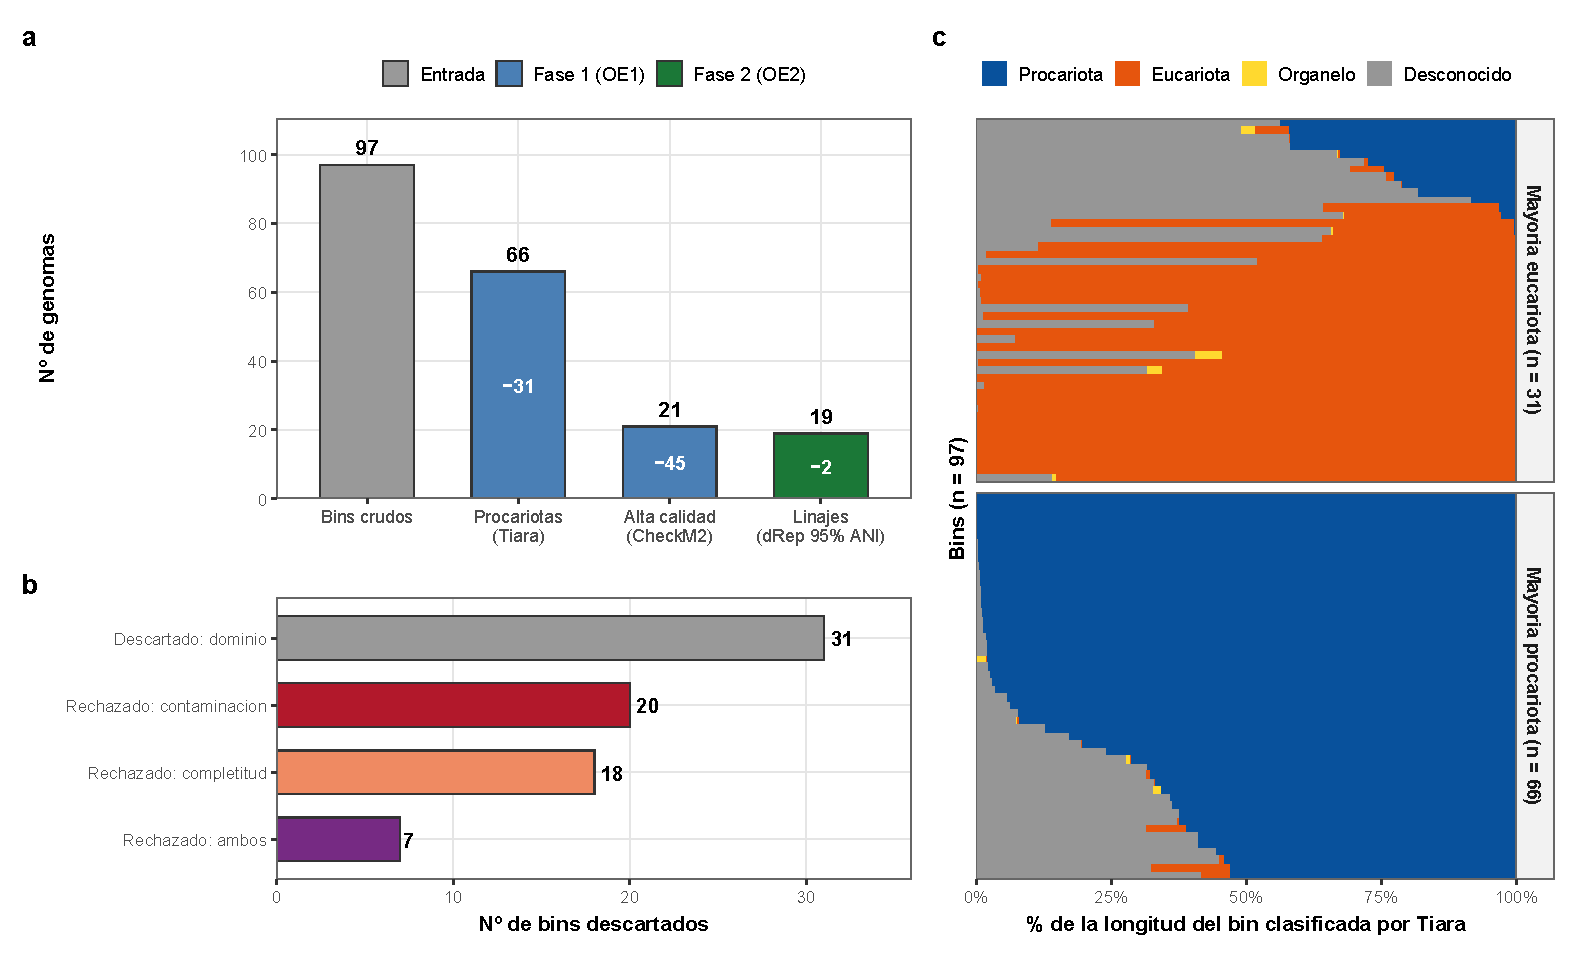
\includegraphics[width=\textwidth]{images/fig1_embudo_seleccion.pdf}
    \caption[Embudo de selección de genomas]{Embudo de selección de genomas
    desde los bins crudos hasta los linajes. \textbf{(a)} Número de genomas que
    sobrevive a cada etapa del flujo: 97 bins crudos procedentes de 22 librerías
    Illumina, 66 con dominio mayoritariamente procariota según Tiara, 21 que
    superan los umbrales de calidad de CheckM2 (completitud superior al
    70\%, contaminación inferior al 5\%) y 19 linajes tras la
    desreplicación con dRep al
    95\% de ANI. Las cifras en blanco indican las pérdidas en cada paso.
    \textbf{(b)} Motivos de descarte de los 76 bins eliminados. \textbf{(c)}
    Composición por dominio de cada uno de los 97 bins según Tiara, expresada
    como porcentaje de la longitud del bin clasificada en cada categoría; los
    bins se separan según su dominio mayoritario y se ordenan por la fracción
    procariota.}
    \label{fig:embudo}
\end{figure}

La Figura~\ref{fig:embudo}(c) muestra que la clasificación por dominio no es
ambigua en la mayoría de los casos: los bins se concentran en los extremos de
la escala, con una fracción procariota cercana al 0\% o al 100\%, y son
pocos los que ocupan posiciones intermedias. Esto respalda la decisión de
aplicar un criterio de mayoría simple sobre la longitud clasificada en lugar de
un umbral más elaborado.

\subsubsection{Calidad y estructura de los 21 genomas seleccionados}

Los 21 genomas retenidos presentan una calidad marcadamente asimétrica respecto
del umbral. La mediana de la completitud alcanza el 99.86\%, con 13 genomas por
encima del 99\% y 5 con completitud estimada del 100.00\%; solo cuatro
quedan por debajo del 80\%. La mediana de la contaminación es del 0.44\%, valor muy por debajo del límite fijado.

\begin{figure}[H]
    \centering
    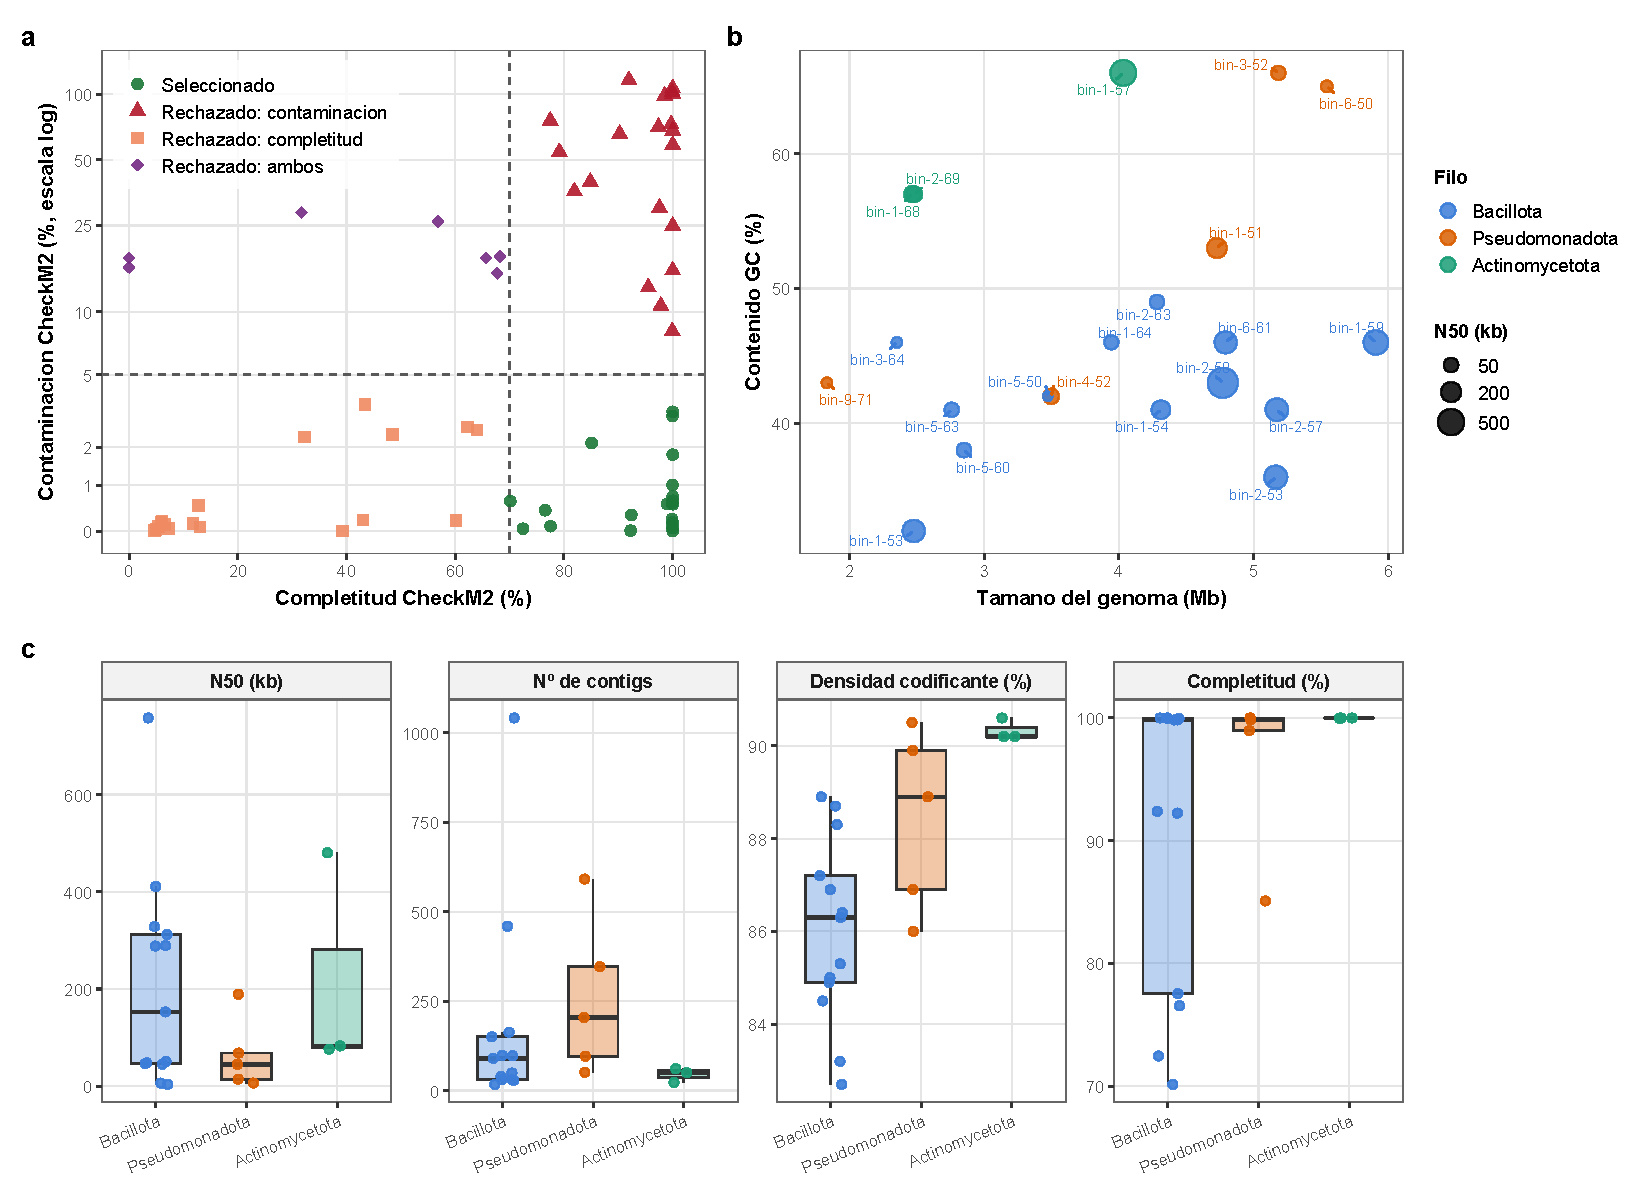
\includegraphics[width=\textwidth]{images/fig2_calidad_genomica.pdf}
    \caption[Calidad y métricas de ensamblaje]{Calidad y métricas de ensamblaje
    de los genomas. \textbf{(a)} Completitud frente a contaminación (CheckM2) de
    los 66 bins procariotas. El eje de contaminación usa escala logarítmica
    ($\log(1+x)$) porque unos pocos bins superan el 60\% y comprimirían la
    región de interés. Las líneas discontinuas marcan los umbrales del estudio
    (completitud igual o superior al 70\%, contaminación inferior al 5\%) y
    la región sombreada, los
    21 genomas seleccionados. \textbf{(b)} Tamaño del genoma frente a contenido
    GC de los 21 genomas seleccionados; el tamaño del punto es proporcional al
    N50 de los contigs y el color indica el filo. \textbf{(c)} Distribución de
    N50, número de contigs, densidad codificante y completitud por filo. Cada
    punto es un genoma; las cajas muestran mediana y cuartiles.}
    \label{fig:calidad}
\end{figure}

La Figura~\ref{fig:calidad}(a) muestra los criterios de contaminación y completitud sobre las distintas poblaciones de bins.

La completitud y la contaminación no describen por completo la utilidad de un
genoma para el análisis pangenómico. La continuidad del ensamblaje sí importa, y
en esa dimensión el conjunto es heterogéneo: el número de contigs va de 17 a
1041, con mediana de 90. Cuatro genomas superan los 300 contigs
(\texttt{bin-5-50} con 1041, \texttt{bin-6-50} con 591, \texttt{bin-3-64} con
459 y \texttt{bin-9-71} con 346).

El caso de \texttt{bin-5-50} muestra que la calidad y la fragmentación de un genoma son aspectos distintos. Este bin tiene una completitud del 76.56\% y una contaminación del 0.44\%, por lo que cumple los criterios del OE1. Sin embargo, sus 3.47 Mb están divididos en más de mil contigs, con una longitud media de solo 3.3 kb.

CheckM2 le asigna una buena calidad porque evalúa principalmente la presencia de genes marcadores, muchos de los cuales pueden encontrarse completos incluso en contigs pequeños. Por tanto, esta métrica no refleja directamente qué tan continuo está el ensamblaje.

El problema aparece en la Fase 3. Cuando un gen queda cortado entre contigs, puede no coincidir correctamente con su versión completa en los genomas de referencia. Como resultado, el análisis pangenómico puede interpretarlo como un gen diferente y clasificarlo como accesorio o incluso exclusivo de la Estela. Así, una alta fragmentación puede generar falsos genes exclusivos, afectando directamente al OE3. Por esta razón, la Fase 3 incluye controles para identificar y descartar estos casos.


Los tamaños genómicos oscilan entre 1.83 y 5.91 Mb, con mediana de 4.03 Mb,
valores compatibles con genomas bacterianos. El extremo inferior
corresponde a \texttt{bin-9-71} (1.83 Mb), cuya completitud del 85.09\%.

\begin{table}[H]
\centering
\small
\caption[Métricas de los 21 MAGs seleccionados]{Métricas de ensamblaje y calidad
genómica de los 21 MAGs seleccionados (completitud superior al 70\% y
contaminación inferior al 5\%).}
\label{tab:bins_seleccionados}
\makebox[\textwidth][c]{%
\begin{tabular}{lrrrrr}
\toprule
\textbf{Bin} & \textbf{Contigs} & \textbf{Longitud (bp)} & \textbf{Dominio} & \textbf{Completitud (\%)} & \textbf{Contaminación (\%)} \\
\midrule
bin-1-51 & 51 & 4.727.435 & prok & 100.00 & 0.00 \\
bin-1-53 & 30 & 2.476.631 & prok & 99.84 & 0.12 \\
bin-1-54 & 49 & 4.312.038 & prok & 92.25 & 0.01 \\
bin-1-57 & 22 & 4.032.412 & prok & 99.99 & 3.23 \\
bin-1-59 & 98 & 5.907.869 & prok & 99.97 & 3.07 \\
bin-1-64 & 163 & 3.944.265 & prok & 99.84 & 0.59 \\
bin-1-68 & 50 & 2.465.224 & prok & 100.00 & 1.79 \\
bin-2-53 & 39 & 5.164.804 & prok & 99.99 & 0.57 \\
bin-2-57 & 28 & 5.172.263 & prok & 99.96 & 1.01 \\
bin-2-58 & 17 & 4.771.531 & prok & 100.00 & 0.06 \\
bin-2-63 & 150 & 4.282.638 & prok & 92.39 & 0.34 \\
bin-2-69 & 61 & 2.481.071 & prok & 99.99 & 0.18 \\
bin-3-52 & 204 & 5.184.467 & prok & 98.97 & 0.58 \\
bin-3-64 & 459 & 2.352.198 & prok & 70.14 & 0.64 \\
bin-4-52 & 96 & 3.497.259 & prok & 99.86 & 0.25 \\
bin-5-50 & 1041 & 3.472.002 & prok & 76.56 & 0.44 \\
bin-5-60 & 97 & 2.849.856 & prok & 77.53 & 0.10 \\
bin-5-63 & 90 & 2.758.939 & prok & 72.46 & 0.05 \\
bin-6-50 & 591 & 5.543.214 & prok & 100.00 & 0.65 \\
bin-6-61 & 30 & 4.792.746 & prok & 100.00 & 0.74 \\
bin-9-71 & 346 & 1.832.072 & prok & 85.09 & 2.13 \\
\bottomrule
\end{tabular}%
}
\end{table}

\subsubsection{Implicancia para el OE1}

El OE1 se cumple. Obtenemos un conjunto de 21 genomas procariotas cuya
completitud y pureza permiten la asignación taxonómica y la comparación
genómica posteriores. Por ese motivo descartamos 78.35\% del material de
partida. La depuración  descarta
organismos que estuvieran presentes en la estela pero que no alcanzan la calidad necesaria para los posteriores análisis. Por lo tanto, la diversidad
real de la fracción viable es mayor que la que estos 21 genomas representan.

El detalle de todos los 97 bins evaluados, con los motivos específicos para su
exclusión, se presenta en el Anexo~\ref{anexo:tabla_completa_bins}.

\subsection{Resultados de la Fase 2: asignación taxonómica y definición de linajes (OE2)}

La Fase 2 se ejecutó en Khipu mediante \texttt{run\_fase2.slurm} (trabajo SLURM
49316) sobre los 21 genomas seleccionados en la fase anterior. El flujo
comprendió la clasificación taxonómica con GTDB-Tk sobre los datos de la versión
R220, la confirmación de especie por ANI, la desreplicación en linajes con dRep
y el cálculo de la prevalencia espacial de cada linaje.

\subsubsection{Composición taxonómica de la fracción viable}

GTDB-Tk clasificó los 21 genomas dentro de tres filos bacterianos. No se detectó
ningún genoma arqueal, lo que resuelve la ambigüedad que
Tiara había dejado abierta en la Fase 1 entre bacterias y arqueas. La
distribución está dominada por Bacillota, con 13 genomas (62\%), seguido de
Pseudomonadota con 5 (24\%) y Actinomycetota con 3 (14\%). Por debajo del
filo, la diversidad es alta en relación con el tamaño de la muestra: los 21
genomas se reparten en 11 órdenes y 17 géneros distintos, y solo cuatro géneros
aportan más de un genoma.

\begin{figure}[H]
    \centering
    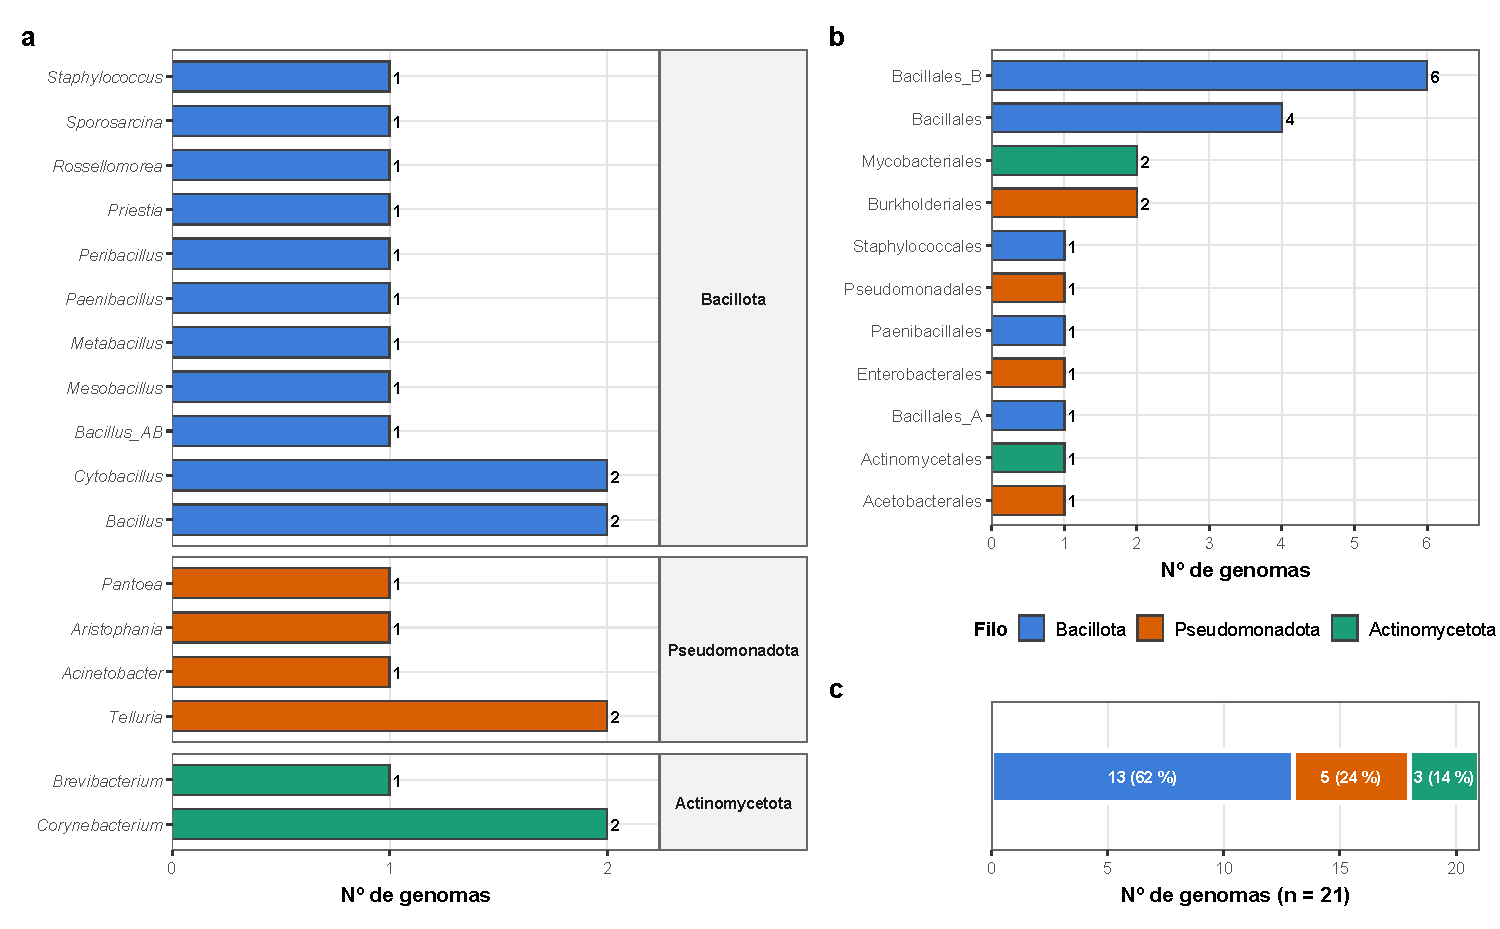
\includegraphics[width=\textwidth]{images/fig7_composicion_taxonomica.pdf}
    \caption[Composición taxonómica]{Composición taxonómica del conjunto de
    genomas seleccionados. \textbf{(a)} Número de genomas por género, agrupados
    por filo. \textbf{(b)} Número de genomas por orden. \textbf{(c)} Reparto de
    los 21 genomas entre los tres filos detectados.}
    \label{fig:composicion}
\end{figure}

El predominio de Bacillota (Figura~\ref{fig:composicion}) es coherente con el
sustrato y con el método de obtención de la muestra. Buena parte de los géneros
recuperados dentro de este filo (\textit{Bacillus}, \textit{Peribacillus},
\textit{Priestia}, \textit{Cytobacillus}, \textit{Metabacillus},
\textit{Rossellomorea}, \textit{Mesobacillus}, \textit{Sporosarcina},
\textit{Paenibacillus}) forma endosporas, una estrategia de resistencia que
favorece la supervivencia sobre una superficie pétrea expuesta a desecación,
radiación ultravioleta y oscilación térmica    \cite{jroundi2020}. 

\subsubsection{Confirmación filogenómica}

\begin{figure}[H]
    \centering
    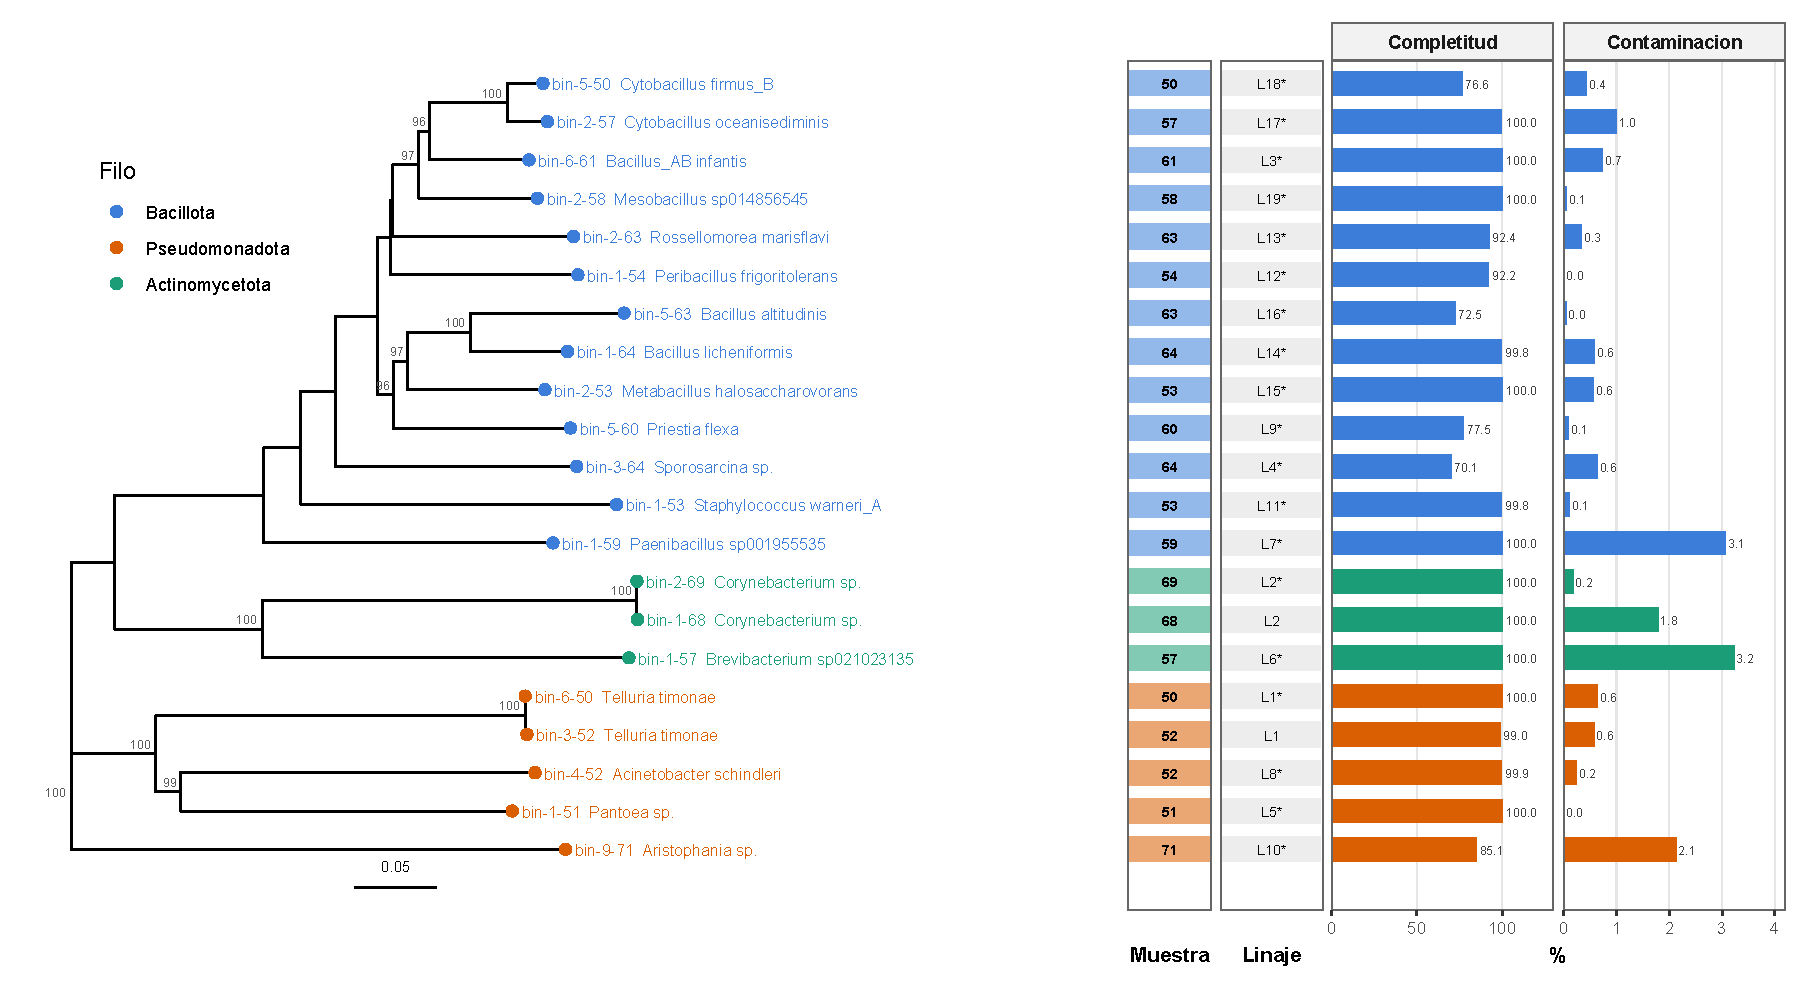
\includegraphics[width=\textwidth]{images/fig3_arbol_filogenomico.pdf}
    \caption[Árbol filogenómico de los 21 genomas]{Árbol filogenómico de los 21
    genomas seleccionados con sus metadatos. Árbol de Neighbor-Joining calculado
    sobre distancias-p a partir del alineamiento concatenado de los 120
    marcadores bacterianos de copia única (bac120, 5035 posiciones) generado por
    GTDB-Tk (datos R220), enraizado en el filo Pseudomonadota. Los números sobre
    las ramas son valores de soporte de \textit{bootstrap} (500 réplicas); solo
    se muestran los iguales o superiores al 70\%. Las columnas de la derecha
    indican, para cada
    genoma, la muestra de origen, el linaje asignado por dRep (el asterisco marca
    el genoma representante del linaje) y los valores de completitud y
    contaminación de CheckM2.}
    \label{fig:arbol}
\end{figure}

La topología del árbol (Figura~\ref{fig:arbol}) es congruente con la asignación
taxonómica: los tres filos se recuperan como grupos separados y los genomas del
mismo género quedan en ramas adyacentes. Los valores de soporte son altos en los
nodos que definen la estructura principal, con \textit{bootstrap} del 100\% en
la separación de los filos y en los pares congenéricos.

El alcance de este resultado es limitado. El árbol es de distancias y se
calculó únicamente sobre los genomas de consulta, sin incorporar genomas de
referencia de GTDB, de modo que verifica la coherencia interna del conjunto pero
no constituye una prueba filogenética independiente de la asignación taxonómica.
Tal como se justificó en el Capítulo IV, el árbol de novo focalizado por linaje,
con referencias del taxón asignado y grupo externo, queda previsto para la
Fase 4.

\subsubsection{Confirmación de especie y candidatos a novedad taxonómica}

Se calculó la Identidad Nucleotídica Promedio de cada genoma frente a su
referencia GTDB más próxima, aplicando los criterios de confirmación de especie
definidos en el Capítulo IV (ANI $\ge 95\%$ y fracción alineada $\ge 65\%$).
Dieciséis de los 21 genomas satisfacen ambos criterios, con valores de ANI entre
95.61\% y 99.99\% y mediana de 98.53\%. Doce de los 16 superan el 98\% de ANI, lo que indica correspondencias con especies
descritas.

\begin{figure}[H]
    \centering
    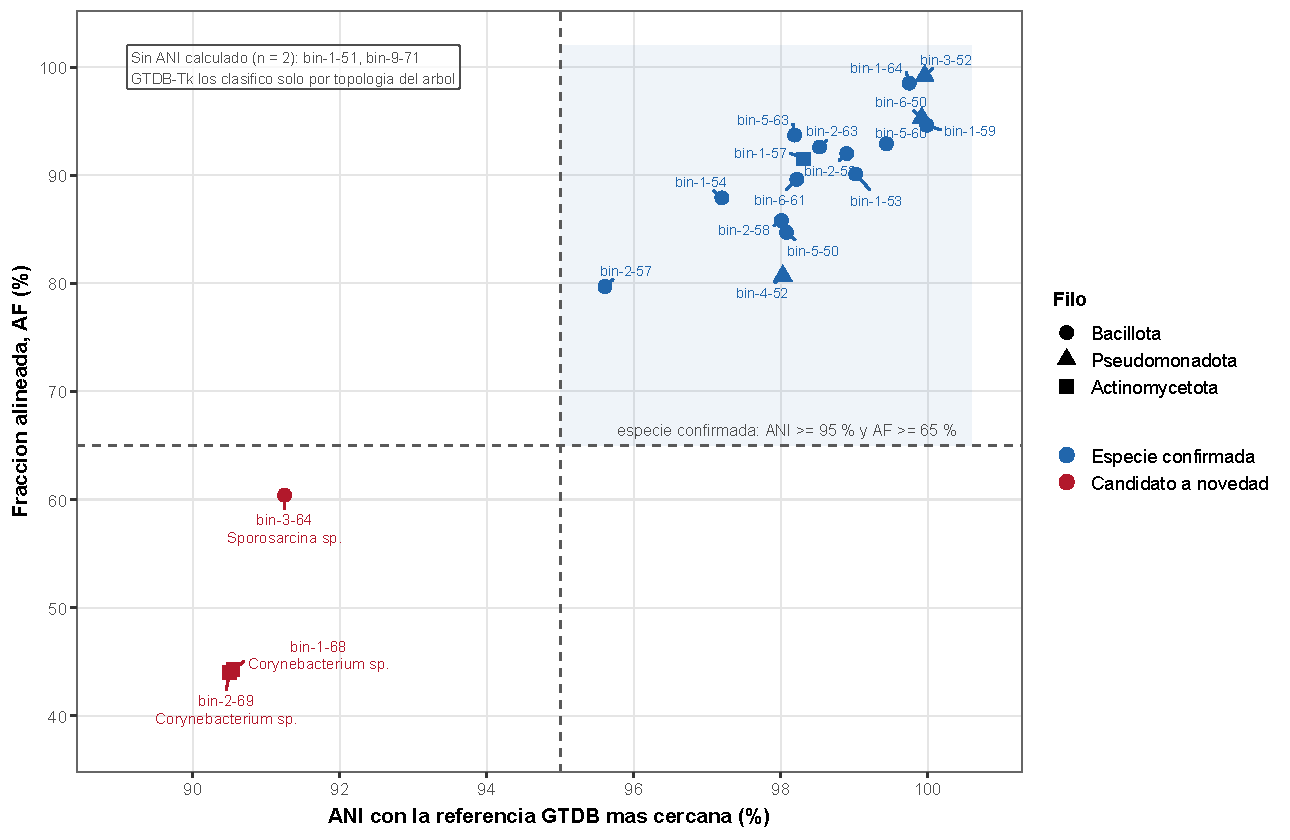
\includegraphics[width=0.85\textwidth]{images/fig5_novedad_taxonomica.pdf}
    \caption[Evaluación de novedad taxonómica]{Evaluación de novedad taxonómica
    frente a la referencia GTDB más cercana. ANI frente a fracción alineada (AF)
    de cada genoma respecto de su referencia GTDB más cercana. Las líneas
    discontinuas marcan los criterios de confirmación de especie (ANI
    igual o superior al 95\% y AF igual o superior al 65\%). Los 16 genomas
    del cuadrante sombreado
    tienen especie confirmada. Dos genomas adicionales (\texttt{bin-1-51},
    \textit{Pantoea} sp., y \texttt{bin-9-71}, \textit{Aristophania} sp.) fueron
    clasificados únicamente por topología del árbol, sin cálculo de ANI, y no
    aparecen representados.}
    \label{fig:novedad}
\end{figure}

Los 5 genomas restantes se distribuyen en dos situaciones distintas
(Figura~\ref{fig:novedad}). Dos de ellos, \texttt{bin-1-51}
(\textit{Pantoea} sp.) y \texttt{bin-9-71} (\textit{Aristophania} sp.), fueron
ubicados por GTDB-Tk mediante la topología del árbol de colocación sin que se
calculara ANI, de modo que su clasificación se detiene en el rango de género por
ausencia de una referencia suficientemente próxima. Por ese motivo, esas secuencias se descartan para la fase 3.

Los otros 3 sí produjeron valores de ANI, pero por debajo del umbral de
especie, y constituyen el hallazgo taxonómico más relevante de esta fase. Los
dos genomas de \textit{Corynebacterium} sp. (\texttt{bin-1-68} y
\texttt{bin-2-69}) alcanzan un ANI de 90.55 y 90.50\% frente a su referencia
más cercana, con fracciones alineadas de apenas 44,3 y 44.0\%. El genoma de
\textit{Sporosarcina} sp. (\texttt{bin-3-64}) queda en 91.25\% de ANI y
60.4\% de AF. Los tres valores de ANI se encuentran por debajo del umbral de similitud utilizado para la circunscripción de especies en GTDB, lo que indica que ninguno de estos genomas puede asignarse a la misma especie que su referencia más cercana. 

En el caso de los \textit{Corynebacterium}
la fracción alineada, inferior al 45\%, indica que menos de la mitad del genoma
encuentra correspondencia en la referencia. Estos genomas son, por tanto,
candidatos a especies no descritas en la versión R220 del GTDB. 

Hacemos énfasis en este resultado porque ambos \textit{Corynebacterium} proceden de muestras
distintas y presentan completitud del 100\%, de modo que la divergencia
observada no es atribuible a una reconstrucción defectuosa.

\subsubsection{Desreplicación y definición de linajes}

La desreplicación con dRep agrupó los 21 genomas en 19 linajes, definidos como
clústeres de especie al 95\% de ANI. Solo dos pares colapsaron.

\begin{figure}[H]
    \centering
    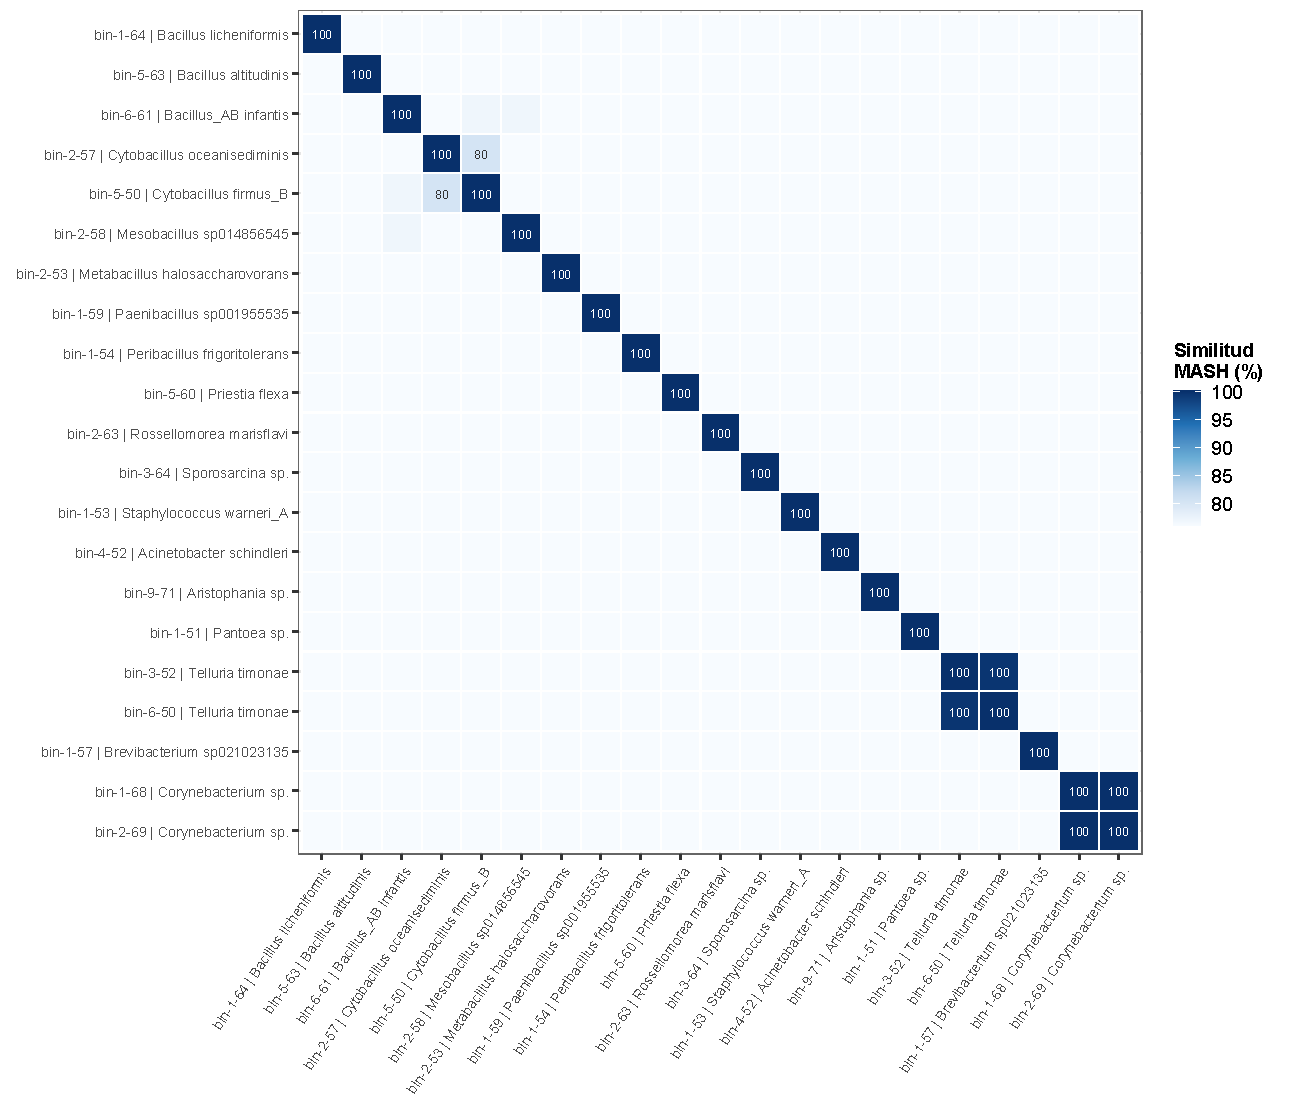
\includegraphics[width=0.9\textwidth]{images/fig4_matriz_mash.pdf}
    \caption[Matriz de similitud genómica]{Matriz de similitud genómica entre
    los 21 genomas seleccionados. Similitud MASH ($100 -$ distancia MASH) entre
    todas las parejas de genomas, ordenadas por filo y género. Solo dos parejas
    presentan similitud máxima: los dos \textit{Telluria timonae} (muestras 50 y
    52) y los dos \textit{Corynebacterium} sp. (muestras 68 y 69). Nota
    metodológica: dRep ejecuta fastANI únicamente dentro de cada clúster primario
    definido por MASH, de modo que no existe una matriz de ANI completa para los
    21 genomas; la matriz de todos contra todos disponible es la de MASH.}
    \label{fig:mash}
\end{figure}

Las dos parejas sometidas a fastANI dentro de su clúster primario superan el
umbral de especie con amplitud: \textit{Corynebacterium} sp.
(\texttt{bin-1-68} $\leftrightarrow$ \texttt{bin-2-69}) alcanza 99.96\% de ANI
con 97.1\% de cobertura del alineamiento, y \textit{Telluria timonae}
(\texttt{bin-3-52} $\leftrightarrow$ \texttt{bin-6-50}), 99.78\% de ANI con
85.2\% de cobertura. Ambas colapsan en un único linaje.

El resto de los genomas resulta mutuamente distante
(Figura~\ref{fig:mash}), incluido el par de \textit{Cytobacillus}
(\texttt{bin-5-50} y \texttt{bin-2-57}), que pese a compartir género se mantiene
como dos linajes separados con una similitud MASH del 80\%. Este es el motivo
de que 21 genomas den lugar a 19 linajes y no a un número menor: la redundancia
entre muestras es baja, y la mayor parte de lo recuperado corresponde a
organismos distintos y no a reconstrucciones repetidas del mismo genoma.

\subsubsection{Prevalencia espacial de los linajes}

\begin{figure}[H]
    \centering
    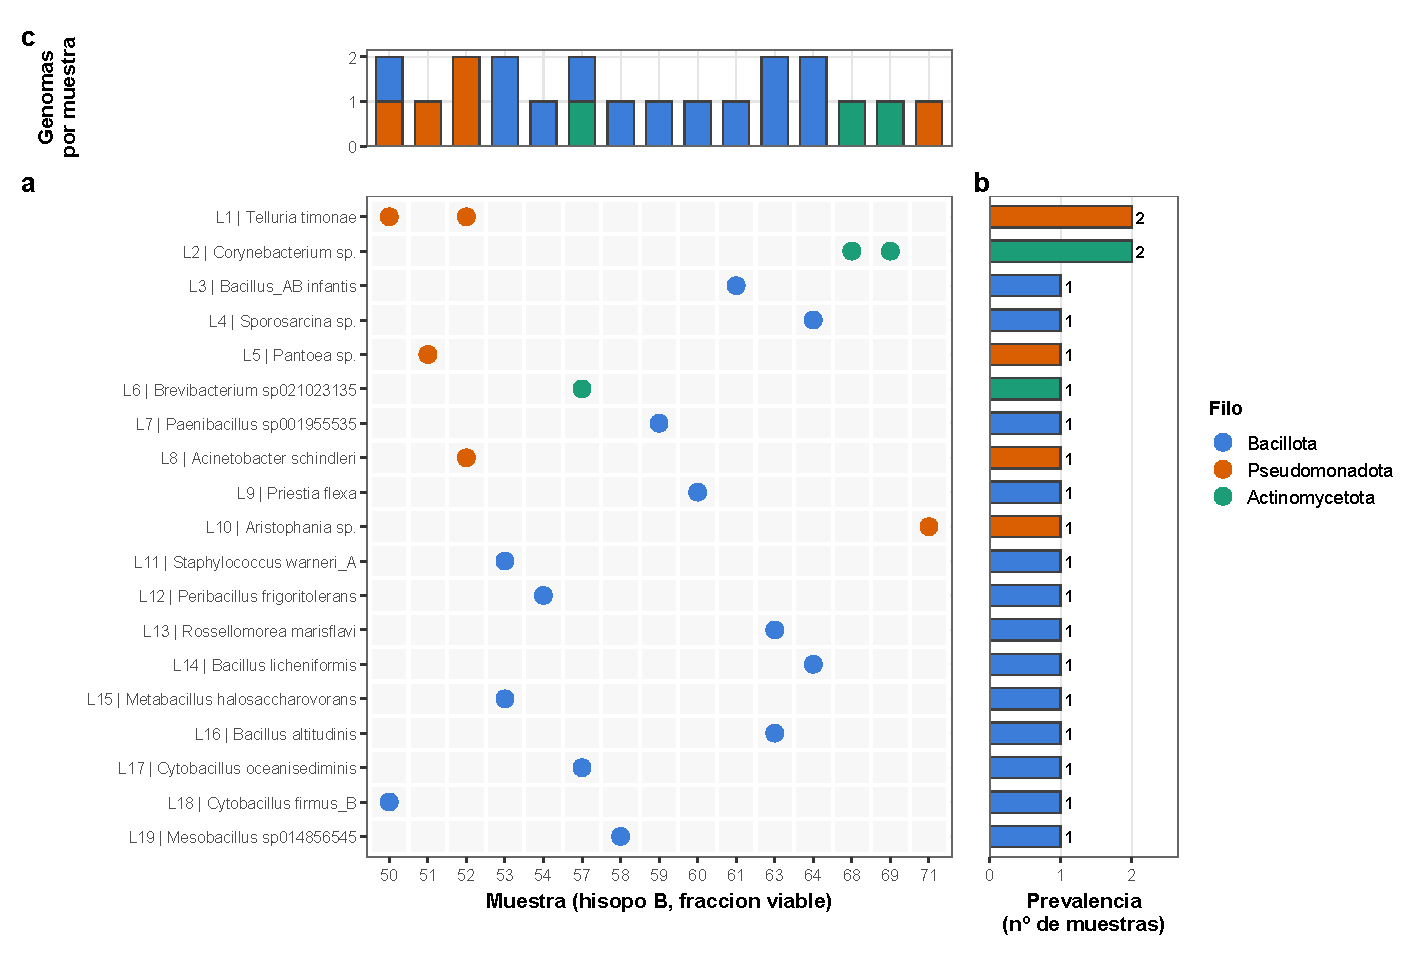
\includegraphics[width=\textwidth]{images/fig6_prevalencia_linajes.pdf}
    \caption[Prevalencia espacial de los linajes]{Prevalencia espacial de los
    linajes. \textbf{(a)} Matriz de presencia de cada linaje (filas, ordenadas
    por prevalencia descendente) en cada muestra (columnas); el color indica el
    filo. \textbf{(b)} Prevalencia de cada linaje, definida como el número de
    muestras distintas en que aparece, coloreada por filo. \textbf{(c)} Número de
    genomas de alta calidad recuperados por muestra, coloreado por filo.
    Limitación: la prevalencia se calcula sobre el número de muestras y no sobre
    zonas físicas de la estela, porque no se dispone de un mapeo
    muestra $\rightarrow$ zona en formato analizable.}
    \label{fig:prevalencia}
\end{figure}

La prevalencia espacial resultó baja en todo el conjunto. Diecisiete de los 19
linajes aparecen en una sola muestra, y solo dos alcanzan una prevalencia de
dos: L1 (\textit{Telluria timonae}, muestras 50 y 52) y L2
(\textit{Corynebacterium} sp., muestras 68 y 69). Ningún linaje se recuperó en
tres o más puntos. Además, de las 22 librerías que produjeron bins, solo 15
aportaron al menos un genoma de alta calidad tras la Fase 1
(Figura~\ref{fig:prevalencia}(c)).

Este resultado limita el poder discriminante de la métrica. Con un rango
efectivo de apenas dos valores, la prevalencia no permite ordenar los linajes ni separar con seguridad a los colonizadores
estables de las detecciones puntuales.

Dos hipotésis resultan compatibles con los datos. La primera es que la comunidad
viable de la estela sea genuinamente heterogénea entre muestras, sin un núcleo de
organismos compartido. La segunda es que la recuperación de genomas de alta calidad sea limitada, de modo que un linaje presente en varias muestras solo pueda reconstruirse con suficiente calidad en una de ellas.

Los datos disponibles no permiten discriminar entre ambas. La segunda tampoco puede descartarse, dado que el flujo retuvo apenas el 21.65\% de los bins iniciales.

Por esta razón, la prevalencia espacial se reporta aquí como caracterización de
la distribución de cada linaje sobre el monumento, pero no se emplea como
criterio para decidir qué especies ingresan al análisis pangenómico. 

Por ese motivo, el criterio de selección de bins para el pangenoma (fase 3) cambia como se explica en la siguiente sección. 

\subsubsection{Implicancia para el OE2}

El OE2 se cumple: los 21 genomas quedan clasificados con resolución de especie
en 16 casos y de género en los 5 restantes, y agrupados en 19 linajes
operativos que constituyen la unidad de análisis de las fases siguientes.

Dos resultados condicionan el diseño posterior. El primero es la baja
redundancia entre muestras: con 19 linajes sobre 21 genomas, y 17 de ellos
representados por un único genoma, no es posible construir un pangenoma
empleando exclusivamente material de la estela. El análisis pangenómico de la
Fase 3 debe apoyarse necesariamente en conjuntos de genomas de referencia
públicos. El segundo es la detección de tres candidatos a especies no descritas,
entre ellos los dos \textit{Corynebacterium} de completitud íntegra, que por
carecer de referencia comparable quedan fuera del análisis pangenómico pero
constituyen un hallazgo reportable por sí mismo.

\begin{table}[H]
\centering
\footnotesize
\setlength{\tabcolsep}{4pt}
\caption[Linajes definidos en la Fase 2]{Linajes definidos en la Fase 2,
ordenados por prevalencia espacial descendente.}
\label{tab:linajes}
\makebox[\textwidth][c]{%
\begin{tabular}{llrlll}
\toprule
\textbf{Linaje} & \textbf{Taxonomía (GTDB)} & \textbf{Prev.} & \textbf{Muestras} & \textbf{Representante} & \textbf{Especie conf.} \\
\midrule
L1  & \textit{Telluria timonae}              & 2 & 50, 52 & bin-6-50 & Sí \\
L2  & \textit{Corynebacterium} sp.           & 2 & 68, 69 & bin-2-69 & No \\
L3  & \textit{Bacillus\_AB infantis}         & 1 & 61 & bin-6-61 & Sí \\
L4  & \textit{Sporosarcina} sp.              & 1 & 64 & bin-3-64 & No \\
L5  & \textit{Pantoea} sp.                   & 1 & 51 & bin-1-51 & --- \\
L6  & \textit{Brevibacterium} sp021023135    & 1 & 57 & bin-1-57 & Sí \\
L7  & \textit{Paenibacillus} sp001955535     & 1 & 59 & bin-1-59 & Sí \\
L8  & \textit{Acinetobacter schindleri}      & 1 & 52 & bin-4-52 & Sí \\
L9  & \textit{Priestia flexa}                & 1 & 60 & bin-5-60 & Sí \\
L10 & \textit{Aristophania} sp.              & 1 & 71 & bin-9-71 & --- \\
L11 & \textit{Staphylococcus warneri\_A}     & 1 & 53 & bin-1-53 & Sí \\
L12 & \textit{Peribacillus frigoritolerans}  & 1 & 54 & bin-1-54 & Sí \\
L13 & \textit{Rossellomorea marisflavi}      & 1 & 63 & bin-2-63 & Sí \\
L14 & \textit{Bacillus licheniformis}        & 1 & 64 & bin-1-64 & Sí \\
L15 & \textit{Metabacillus halosaccharovorans} & 1 & 53 & bin-2-53 & Sí \\
L16 & \textit{Bacillus altitudinis}          & 1 & 63 & bin-5-63 & Sí \\
L17 & \textit{Cytobacillus oceanisediminis}  & 1 & 57 & bin-2-57 & Sí \\
L18 & \textit{Cytobacillus firmus\_B}        & 1 & 50 & bin-5-50 & Sí \\
L19 & \textit{Mesobacillus} sp014856545      & 1 & 58 & bin-2-58 & Sí \\
\bottomrule
\end{tabular}%
}

\vspace{0.5em}
\begin{minipage}{0.95\textwidth}
\footnotesize
\textit{Nota.} Prev.: prevalencia espacial, número de muestras distintas que
aportan al menos un genoma al linaje. Especie conf.: confirmación de especie por
ANI igual o superior al 95\% y AF igual o superior al 65\%; el guion indica
los linajes clasificados por
topología del árbol, sin cálculo de ANI. Los sufijos \texttt{\_A} y \texttt{\_B}
y los epítetos alfanuméricos del tipo \texttt{sp}$\langle$dígitos$\rangle$
corresponden a la nomenclatura propia del GTDB.
\end{minipage}
\end{table}

\subsection{Sensibilidad de los resultados a los umbrales elegidos}

Los resultados anteriores corresponden a una sola configuración. Esta sección
responde a una pregunta distinta: cuánto habrían cambiado esos resultados con
otros umbrales. La respuesta permite saber si el conjunto de 21 genomas es un
resultado estable o el producto de una elección afortunada.

\subsubsection{Umbrales de calidad genómica}

Los escenarios E1 y E2 recalcularon la selección sobre los 66 bins procariotas
variando de forma simultánea los dos umbrales de CheckM2. La
Tabla~\ref{tab:sensibilidad_calidad} muestra el resultado.

\begin{table}[H]
\centering
\small
\caption[Sensibilidad a los umbrales de calidad]{Número de genomas retenidos
sobre los 66 bins procariotas al variar los umbrales de completitud y
contaminación. La celda en negrita corresponde al caso base.}
\label{tab:sensibilidad_calidad}
\begin{tabular}{lrrrr}
\toprule
\textbf{Completitud} & \textbf{Cont. $<1\%$} & \textbf{Cont. $<3\%$} & \textbf{Cont. $<5\%$} & \textbf{Cont. $<10\%$} \\
\midrule
$> 50\%$ & 17 & 22 & 24 & 25 \\
$> 60\%$ & 17 & 22 & 24 & 25 \\
$> 70\%$ & 16 & 19 & \textbf{21} & 22 \\
$> 80\%$ & 12 & 15 & 17 & 18 \\
$> 90\%$ & 12 & 14 & 16 & 17 \\
$> 95\%$ & 10 & 12 & 14 & 15 \\
\bottomrule
\end{tabular}
\end{table}

El conjunto seleccionado resulta poco sensible al umbral de completitud. Bajarlo
de 70 a 50\% solo añade tres genomas. Subirlo de 70 a 90\% solo retira cinco. La
explicación está en la distribución de la completitud dentro del conjunto
retenido, descrita en la Sección 7.2.1: la mediana alcanza el 99.86\% y trece
genomas superan el 99\%. La mayoría de los genomas seleccionados está lejos del
umbral, de modo que moverlo no los afecta.

El umbral de contaminación pesa más. Entre 1 y 5\% el conjunto pasa de 16 a 21
genomas, y cinco genomas dependen por completo de dónde se ponga ese límite. La
contaminación es también el criterio que rechazó más bins en el caso base, con
20 exclusiones por ese solo motivo. En conjunto, la contaminación es el
parámetro que gobierna el tamaño final del conjunto, y no la completitud.

Aumentar la contaminación hasta el 10\% habría añadido un solo genoma frente al
caso base. Esto indica que el límite del 5\% no está descartando material útil
que un criterio algo más permisivo habría recuperado. Entre 5 y 10\% de
contaminación casi no hay bins.

\subsubsection{Criterio de discriminación por dominio}

El caso base decide el dominio de cada bin por mayoría simple sobre la longitud
clasificada. El escenario E3 reemplazó ese criterio por un umbral explícito
sobre la fracción procariota. La Tabla~\ref{tab:sensibilidad_dominio} compara
ambas opciones.

\begin{table}[H]
\centering
\small
\caption[Sensibilidad del criterio de dominio]{Número de bins retenidos, sobre
los 97 de partida, según el criterio de discriminación por dominio.}
\label{tab:sensibilidad_dominio}
\begin{tabular}{lr}
\toprule
\textbf{Criterio} & \textbf{Bins retenidos} \\
\midrule
Mayoría simple (caso base)        & 66 \\
Fracción procariota $> 25\%$      & 56 \\
Fracción procariota $> 40\%$      & 54 \\
Fracción procariota $> 50\%$      & 50 \\
Fracción procariota $> 60\%$      & 44 \\
Fracción procariota $> 75\%$      & 34 \\
Fracción procariota $> 90\%$      & 30 \\
\bottomrule
\end{tabular}
\end{table}

Este es el punto del flujo más sensible al criterio elegido. La mayoría simple
retiene 66 bins, mientras que exigir más de la mitad de la longitud clasificada
como procariota retendría 50. La diferencia de 16 bins se explica porque la
mayoría simple compara la fracción procariota contra las fracciones eucariota,
organelar y desconocida por separado. Un bin con 40\% de longitud procariota,
30\% eucariota y 30\% desconocida tiene mayoría procariota, aunque menos de la
mitad de su longitud lo sea.

Hay 22 bins cuya fracción procariota queda entre el 25 y el 75\%. La afirmación
de la Sección 7.2.1 sobre la concentración de los bins en los extremos de la
escala describe bien la tendencia general, pero este grupo intermedio existe y
conviene dimensionarlo.

El efecto sobre el resultado final es menor de lo que sugieren estas cifras. El
filtro de calidad de CheckM2 actúa después y elimina de todos modos los bins con
mezcla de dominios, porque esa mezcla aparece como contaminación. El criterio de
dominio afecta sobre todo al costo de cómputo de la etapa siguiente, ya que
determina cuántos bins se someten a CheckM2.

\subsubsection{Umbral de ANI para la definición de linaje}

El escenario E4 varió el umbral de ANI con el que dRep agrupa genomas en
linajes. El resultado es que el número de linajes no cambia: se mantiene en 19
para umbrales de 95, 98, 99 y 99.5\% de ANI.

La razón está en los valores observados. Solo dos parejas de genomas fueron
comparadas con fastANI dentro de su clúster primario, y ambas presentan
identidades muy altas: 99.95\% entre los dos \textit{Corynebacterium} y 99.78\%
entre los dos \textit{Telluria timonae}. Ambas parejas siguen colapsando incluso
con un umbral del 99.5\%. El resto de los genomas está tan separado que ningún
umbral razonable los uniría.

Por lo tanto, la definición de linaje es insensible al umbral dentro de este
conjunto. Este resultado refuerza la conclusión de la Sección 7.2.2 sobre la
baja redundancia del material recuperado.

\subsubsection{Continuidad del ensamblaje}

El caso base no filtra por número de contigs. El escenario E5 añadió ese filtro
para medir su efecto. Aplicar un límite de 300 contigs sobre los 21 genomas
seleccionados dejaría 17. Saldrían \texttt{bin-5-50} (1041 contigs),
\texttt{bin-6-50} (591), \texttt{bin-3-64} (459) y \texttt{bin-9-71} (346).

Este filtro no se aplicó en la Fase 1 por una razón concreta. Los cuatro genomas
afectados incluyen a \texttt{bin-6-50}, representante del linaje más prevalente,
y a \texttt{bin-9-71}, único representante de su género. Excluirlos habría
reducido la descripción taxonómica de la comunidad, que es el objetivo del OE2,
a cambio de una mejora que solo importa en el análisis pangenómico posterior. La
decisión fue conservarlos en las Fases 1 y 2 y trasladar el control de
continuidad a la etapa donde la fragmentación sí genera un error, tal como se
discute en la Sección 7.2.1 a propósito de \texttt{bin-5-50}.

\subsection{Iteraciones de diseño derivadas de los resultados}

El diseño del flujo no se mantuvo fijo durante la ejecución. Dos resultados
obligaron a modificarlo. Esta sección documenta ambos casos siguiendo el ciclo
de prueba, evaluación y rediseño.

Conviene precisar en qué consiste cada cambio. El diseño descrito en el
Capítulo IV es el punto de partida, y las pruebas de este capítulo son
precisamente el mecanismo previsto para ponerlo a prueba. En los dos casos siguientes, los cambios se hicieron a partir de resultados obtenidos durante el análisis. Uno se debió a un requerimiento de memoria mayor al disponible y el otro a una métrica que no permitió diferenciar adecuadamente los resultados. Para mantener la trazabilidad, se presentan por separado el diseño original, la evidencia que motivó el cambio y el diseño corregido.


\subsubsection{Primera iteración: alcance del árbol filogenómico}

El diseño inicial contemplaba construir un árbol \textit{de novo} que incluyera
los genomas propios junto con el conjunto completo de genomas de referencia del
dominio bacteriano de GTDB. La prueba mostró que ese cálculo no cabe en los
98 GB de memoria asignados a la cuenta.

La evaluación de ese fallo distingue dos problemas. El primero es de recursos y
no admite solución dentro de la cuota disponible. El segundo es de alcance: el
objetivo del OE2 no requiere un árbol del dominio completo, sino verificar la
coherencia de las asignaciones taxonómicas.

El rediseño consistió en dos cambios. Para la Fase 2 se calculó un árbol de
distancias sobre el alineamiento concatenado de los 120 marcadores, restringido
a los nuestros genomas. Ese árbol es el que aparece en la
Figura~\ref{fig:arbol} y cumple la función de verificación interna.

\subsubsection{Segunda iteración: criterio de selección de linajes para el pangenoma}

El diseño original preveía seleccionar los linajes del análisis pangenómico por
prevalencia espacial. La lógica era que un linaje presente en varios puntos del
monumento resulta más relevante para el biodeterioro que una detección aislada.

La prueba invalidó ese criterio. Como muestra la Sección 7.2.2, diecisiete de
los 19 linajes aparecen en una sola muestra y solo dos alcanzan una prevalencia
de dos. Con
esa distribución no es posible construir un ranking ni separar bacterias colonizadoras
estables de detecciones puntuales.

La evaluación de este resultado identificó además una restricción más básica.
Con 19 linajes sobre 21 genomas, y 17 de ellos representados por un único
genoma, el material propio no alcanza para construir ningún pangenoma. El
análisis pangenómico depende necesariamente de genomas de referencia públicos,
de modo que el criterio de selección debe incorporar la disponibilidad de esas
referencias.

El rediseño reemplazó la prevalencia espacial por la disponibilidad genómica
pública. Un linaje ingresa al análisis pangenómico si existe para su especie un
número suficiente de genomas públicos de calidad adecuada. El umbral adoptado es
de 15 genomas.

Es importante mencionar que la inclusión de genomas filogenéticamente redundantes infla de
forma artificial el tamaño del core y subestima el genoma accesorio, lo que
puede llevar a describir como cerrado un pangenoma que en realidad es
abierto~\cite{guerra2026}. Quince genomas redundantes no equivalen a quince
genomas informativos. Por lo tanto, este parámetro está abierto a iteración. 

La prevalencia espacial se conserva como resultado descriptivo del OE2 y se
reporta en la Tabla~\ref{tab:linajes}, pero deja de cumplir función de criterio
de selección. 

\section{Verificación del cumplimiento de las especificaciones técnicas}

Esta sección
dictamina si el desempeño del \textit{pipeline} alcanza los valores comprometidos. Las
especificaciones se derivan de los objetivos específicos OE1 y OE2 y son las
únicas que admiten una verificación cuantitativa directa. La
Tabla~\ref{tab:matriz_especificaciones} cruza cada especificación con su método
de verificación y con el resultado obtenido.

\begin{table}[H]
\centering
\footnotesize
\setlength{\tabcolsep}{4pt}
\caption[Matriz de verificación de especificaciones técnicas]{Matriz de
verificación del cumplimiento de las especificaciones técnicas.}
\label{tab:matriz_especificaciones}
\makebox[\textwidth][c]{%
\begin{tabular}{p{3.5cm}p{3.2cm}p{2.6cm}p{3.4cm}c}
\toprule
\textbf{Especificación} & \textbf{Método de verificación} & \textbf{Objetivo} & \textbf{Resultado obtenido} & \textbf{Cumple} \\
\midrule
Calidad del conjunto final de genomas &
CheckM2 sobre cada genoma &
Completitud $> 70\%$ y contaminación $< 5\%$ &
21 de 21 genomas; mediana de completitud 99.86\% y de contaminación 0.44\% &
Sí \\
\addlinespace
Resolución taxonómica de la asignación &
GTDB-Tk sobre datos R220, con confirmación por ANI &
Asignación al menos a nivel de género &
21 de 21 a género; 16 de 21 con especie confirmada (ANI $\ge 95\%$, AF $\ge 65\%$) &
Sí \\
\addlinespace
Trazabilidad entre genoma y muestra de origen &
Registro de correspondencia generado en la normalización de nombres &
21 de 21 genomas &
21 de 21 genomas vinculados a su librería de origen &
Sí \\
\addlinespace
Definición de unidades de análisis no redundantes &
Desreplicación con dRep al 95\% de ANI &
Conjunto sin genomas duplicados &
19 linajes sobre 21 genomas; dos parejas colapsadas &
Sí \\
\addlinespace
Reproducibilidad de la ejecución &
Registro de versiones y control de versiones del código &
Versiones de herramientas y bases registradas &
Registro de versiones por fase; scripts y resultados versionados en repositorio &
Sí \\
\bottomrule
\end{tabular}%
}
\end{table}

\section{Verificación del cumplimiento de restricciones}

Las restricciones son límites que el diseño no podía cruzar, a diferencia de las
especificaciones, que son metas de desempeño. La
Tabla~\ref{tab:matriz_restricciones} verifica cada una.

\begin{table}[H]
\centering
\footnotesize
\setlength{\tabcolsep}{4pt}
\caption[Matriz de verificación de restricciones]{Matriz de verificación del
cumplimiento de las restricciones del proyecto.}
\label{tab:matriz_restricciones}
\makebox[\textwidth][c]{%
\begin{tabular}{p{3.2cm}p{3.0cm}p{4.4cm}c}
\toprule
\textbf{Restricción} & \textbf{Origen} & \textbf{Forma en que el diseño la respeta} & \textbf{Cumple} \\
\midrule
Cuota de cómputo de 32 núcleos, 98 GB de memoria y 24 h por trabajo &
Política de asignación del clúster Khipu &
Ambas fases se ejecutaron como trabajos únicos y finalizaron dentro del límite de tiempo asignado. El árbol de referencia completo se reemplazó por un árbol focalizado tras exceder la memoria disponible &
Sí \\
\addlinespace
Los nodos de cómputo no tienen acceso a internet &
Arquitectura del clúster &
Las bases de datos de CheckM2 y GTDB R220 se descargaron en el nodo de login antes de la ejecución. Ninguna etapa del flujo requiere conexión durante el cálculo &
Sí \\
\addlinespace
No se dispone de las lecturas crudas de secuenciación &
Condición de entrega del material por el centro de secuenciación &
El flujo se diseñó para operar sobre bins ya ensamblados. No se recalculan coberturas ni se rehace el ensamblaje ni el \textit{binning} &
Sí \\
\addlinespace
El conjunto de muestras es cerrado y no ampliable &
Condición de acceso al monumento &
El diseño trabaja con las 22 librerías disponibles. Las limitaciones de prevalencia se reportan como tales y no se compensan con muestreo adicional &
Sí \\
\addlinespace
Uso exclusivo de software de licencia libre y bases de datos públicas &
Restricción presupuestal del proyecto &
Todas las herramientas y bases empleadas son de acceso abierto &
Sí \\
\bottomrule
\end{tabular}%
}
\end{table}


% ======================================================================
% ENTRADAS BIBLIOGRAFICAS NUEVAS - agregar a referencias.bib
% ======================================================================
%
% @article{gautreau2020,
%   author  = {Gautreau, Guillaume and Bazin, Adelme and Gachet, Mathieu and
%              Planel, Remi and Burlot, Laura and Dubois, Mathieu and
%              Perrin, Amandine and Medigue, Claudine and Calteau, Alexandra and
%              Cruveiller, Stephane and Matias, Catherine and Ambroise, Christophe and
%              Rocha, Eduardo P. C. and Vallenet, David},
%   title   = {{PPanGGOLiN}: Depicting microbial diversity via a partitioned pangenome graph},
%   journal = {PLOS Computational Biology},
%   volume  = {16},
%   number  = {3},
%   pages   = {e1007732},
%   year    = {2020},
%   doi     = {10.1371/journal.pcbi.1007732}
% }
%
% @article{tettelin2005,
%   author  = {Tettelin, Herve and Masignani, Vega and Cieslewicz, Michael J. and others},
%   title   = {Genome analysis of multiple pathogenic isolates of {Streptococcus agalactiae}: Implications for the microbial pan-genome},
%   journal = {Proceedings of the National Academy of Sciences},
%   volume  = {102},
%   number  = {39},
%   pages   = {13950--13955},
%   year    = {2005},
%   doi     = {10.1073/pnas.0506758102}
% }
%
% @article{guerra2026,
%   author  = {Guerra, Alberto},
%   title   = {The pangenome: a statistical model, not a fixed biological property},
%   journal = {Bioinformatics Advances},
%   volume  = {6},
%   number  = {1},
%   pages   = {vbag069},
%   year    = {2026},
%   doi     = {10.1093/bioadv/vbag069}
% }

%\customchapter{CONCLUSIONES} 

Lorem ipsum dolor sit amet, dicant volutpat vulputate sea at. Et nam volumus voluptua, ea noster omnesque has. Qui ut graeci melius platonem. Sit fugit prompta dignissim cu. Soluta meliore repudiare vis in, eum id liber maiestatis contentiones.

Ea sit suas melius verear. Fugit facilisis at vel, apeirian appellantur ex nec. Vis id quis elit qualisque. Ludus sadipscing eu eum.

Ea inani insolens dissentiunt eos, wisi efficiendi ex vim, modus justo inani et pro. Eam at modus definiebas, id eos philosophia disputationi, eu qui facete habemus. In dico unum neglegentur mea, ne phaedrum disputationi his. Tibique deseruisse mel ne, latine aperiri phaedrum duo ex. Erant corrumpit ut duo, in erant possim reprehendunt nec. Aeque nonumes minimum te eam, possim constituto qui ei, in has suas quidam molestie.

Vel no intellegat voluptaria, ei sed causae scaevola comprehensam. No erant cetero dissentiet per, mei an nulla scaevola. Euismod delicata vis eu, in odio docendi persecuti sea. Eos fabellas accusata at. His eu reque altera sadipscing, id ius regione lobortis expetenda, minim timeam dignissim vix eu.

Unum duis definitiones vel in. Nulla dicit mei ea, odio nulla an pri. Cu docendi torquatos usu. Possit maiorum rationibus ea duo, eu vitae primis postulant sed, mel erat officiis principes an. Pro saepe regione volumus id, debet reformidans ex his. Sale altera moderatius duo ea, an fastidii volutpat per, et mel maiorum corpora.

Modo malis et eam. Veniam equidem mei ad, mucius facilisi et pro. Postea eripuit neglegentur vis no. Id vis quis eleifend appellantur, sit integre singulis ei.
%\chapter*{\center \Large RECOMENDACIONES} 
\addcontentsline{toc}{section}{\bfseries RECOMENDACIONES} 
\markboth{RECOMENDACIONES}{RECOMENDACIONES} 

Lorem ipsum dolor sit amet, mei no laboramus gloriatur, no timeam euripidis qui, eu eos aperiam patrioque accommodare. Mei probo accommodare an, ex case minim salutatus sit. Ad doming impetus mei, placerat verterem has no. His assum quaeque et, ea aliquid dissentiet eum. Copiosae evertitur cum te, sea clita disputationi ea.

Libris ridens malorum cu vis. Per vitae eirmod cotidieque cu. Cum unum mucius alterum eu, nam enim regione appellantur id. Cum putant dignissim te, est dolore essent definiebas ei. Facilisi convenire vix in, dictas delenit et per. Pro tota affert argumentum cu. % sección opcional

%% ============================================================================
\renewcommand{\bibname}{\hfill\Large\bf{REFERENCIAS BIBLIOGRÁFICAS}\hfill}

\bibliographystyle{IEEEtran} % Estableciendo el estilo de citas IEEEtram.

\bibliography{referencias} % Recibe las referencias de IEEE

\chapter*{\center \Large ANEXOS} 
\addcontentsline{toc}{section}{\bfseries ANEXOS} 
\markboth{ANEXOS}{ANEXOS} 

\section*{ANEXO ABET ING 1 - Resolución de problemas}
\addcontentsline{toc}{section}{Resolución de problemas}
Para filtrar por dominio los MAGs obtenidos se evaluaron las siguientes herramientas:

Tiara: Es una herramienta de clasificación de secuencias metagenómicas basada en \textit{deep learning} que permite separar contigs en categorías como arqueas, bacterias, procariotas, eucariotas, orgánulos y secuencias desconocidas mediante un esquema de dos etapas \cite{karlicki2022tiara}. Según su publicación original, mostró un rendimiento similar a EukRep para la clasificación de secuencias procariotas, pero superior para secuencias eucariotas, además de requerir menor tiempo de cómputo \cite{karlicki2022tiara}. Su principal ventaja es que no solo discrimina entre eucariotas y procariotas, sino que también puede identificar ADN organelar, lo que la hace especialmente útil en metagenomas complejos. Sin embargo, al basarse principalmente en patrones de composición de secuencia, puede presentar ambigüedad en linajes evolutivamente inusuales o muy cercanos a eucariotas, por lo que sus resultados deben interpretarse como una clasificación preliminar y no como una asignación taxonómica definitiva.

Whokaryote: Es un clasificador diseñado para distinguir contigs eucariotas y procariotas a partir de características de estructura génica, como la densidad génica, la distancia intergénica y la longitud de los genes, utilizando un modelo de \textit{random forest} \cite{pronk2022whokaryote}. A diferencia de Tiara y EukRep, que dependen sobre todo de frecuencias de \textit{k-mers}, Whokaryote se apoya en diferencias biológicas más interpretables entre ambos dominios. En su artículo, los autores reportan una exactitud cercana al 97\%, indicando además que su desempeño es comparable al de Tiara y EukRep, con la ventaja adicional de aportar una validación independiente basada en otro tipo de señal \cite{pronk2022whokaryote}. Su principal fortaleza es precisamente esa complementariedad metodológica, ya que puede ayudar a confirmar o cuestionar clasificaciones obtenidas por herramientas basadas en composición. Como desventaja, depende de rasgos derivados de genes predichos, por lo que su ejecución es menos directa y puede ser más sensible a la calidad del ensamblado y de la predicción génica subyacente.

EukRep: Es una de las herramientas pioneras para separar secuencias eucariotas de procariotas en ensamblados metagenómicos, utilizando frecuencias de \textit{k-mers} y un clasificador lineal tipo SVM \cite{west2018genomereconstruction}. Su objetivo principal es servir como filtro inicial para recuperar secuencias eucariotas y permitir después el uso de \textit{pipelines} de anotación y análisis específicos para eucariotas. En su publicación original, mostró una exactitud global cercana al 90\% con fragmentos de 3 kb y de aproximadamente 98\% con fragmentos de 20 kb, lo que evidencia un mejor rendimiento en contigs largos \cite{west2018genomereconstruction}. Su ventaja principal es que se trata de una herramienta ampliamente reconocida y adoptada en estudios de recuperación de genomas eucariotas a partir de metagenomas. No obstante, sus limitaciones incluyen un menor desempeño relativo frente a Tiara en la clasificación de eucariotas y la ausencia de una clasificación explícita de secuencias organelares, además de que su precisión puede disminuir en fragmentos más cortos o en ensamblados altamente fragmentados.
\\

\section*{ANEXO ABET ING 5 - Trabajo en equipo}

\addcontentsline{toc}{section}{Trabajo en equipo}
En este anexo se presenta la evidencia del trabajo colaborativo desarrollado durante la ejecución del proyecto. Se podrán incluir reuniones de coordinación, distribución de tareas, seguimiento de avances y productos elaborados en conjunto.

% Agrega aquí tablas, imágenes, capturas o descripciones según tu evidencia.
% Ejemplo:
\begin{figure}[H]
    \centering
    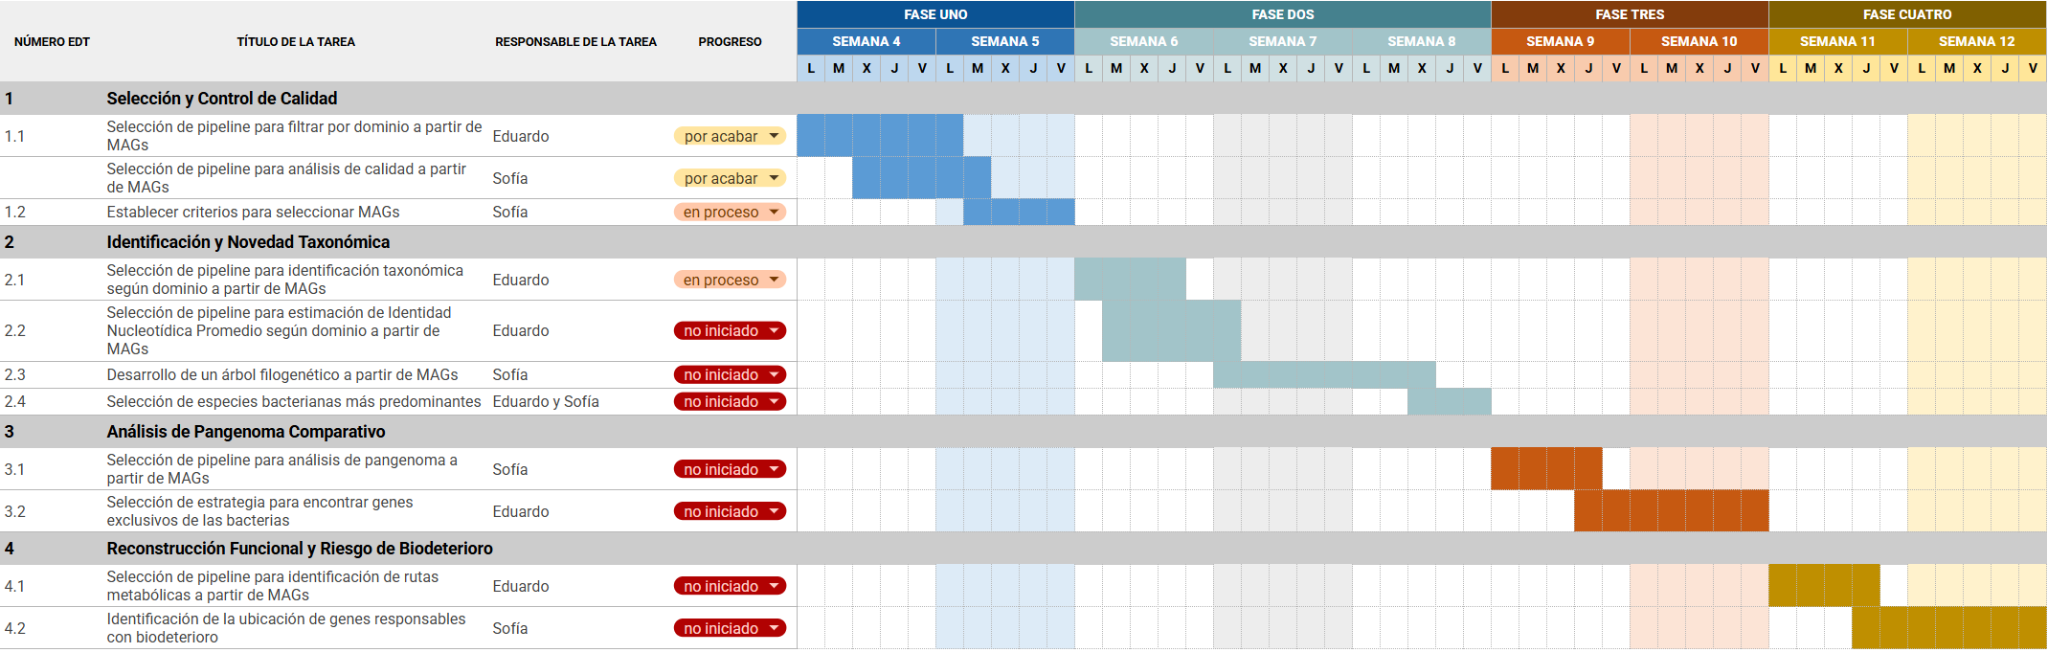
\includegraphics[width=0.8\textwidth]{images/0.png}
    \caption{Diagrama de Gantt del trabajo en equipo durante el desarrollo del proyecto.}
    \label{fig:evidencia_equipo}
\end{figure}


\section*{ANEXO ABET ING 6 --- Experimentación}
\addcontentsline{toc}{section}{Experimentación}
\begin{figure}[H]
    \centering
    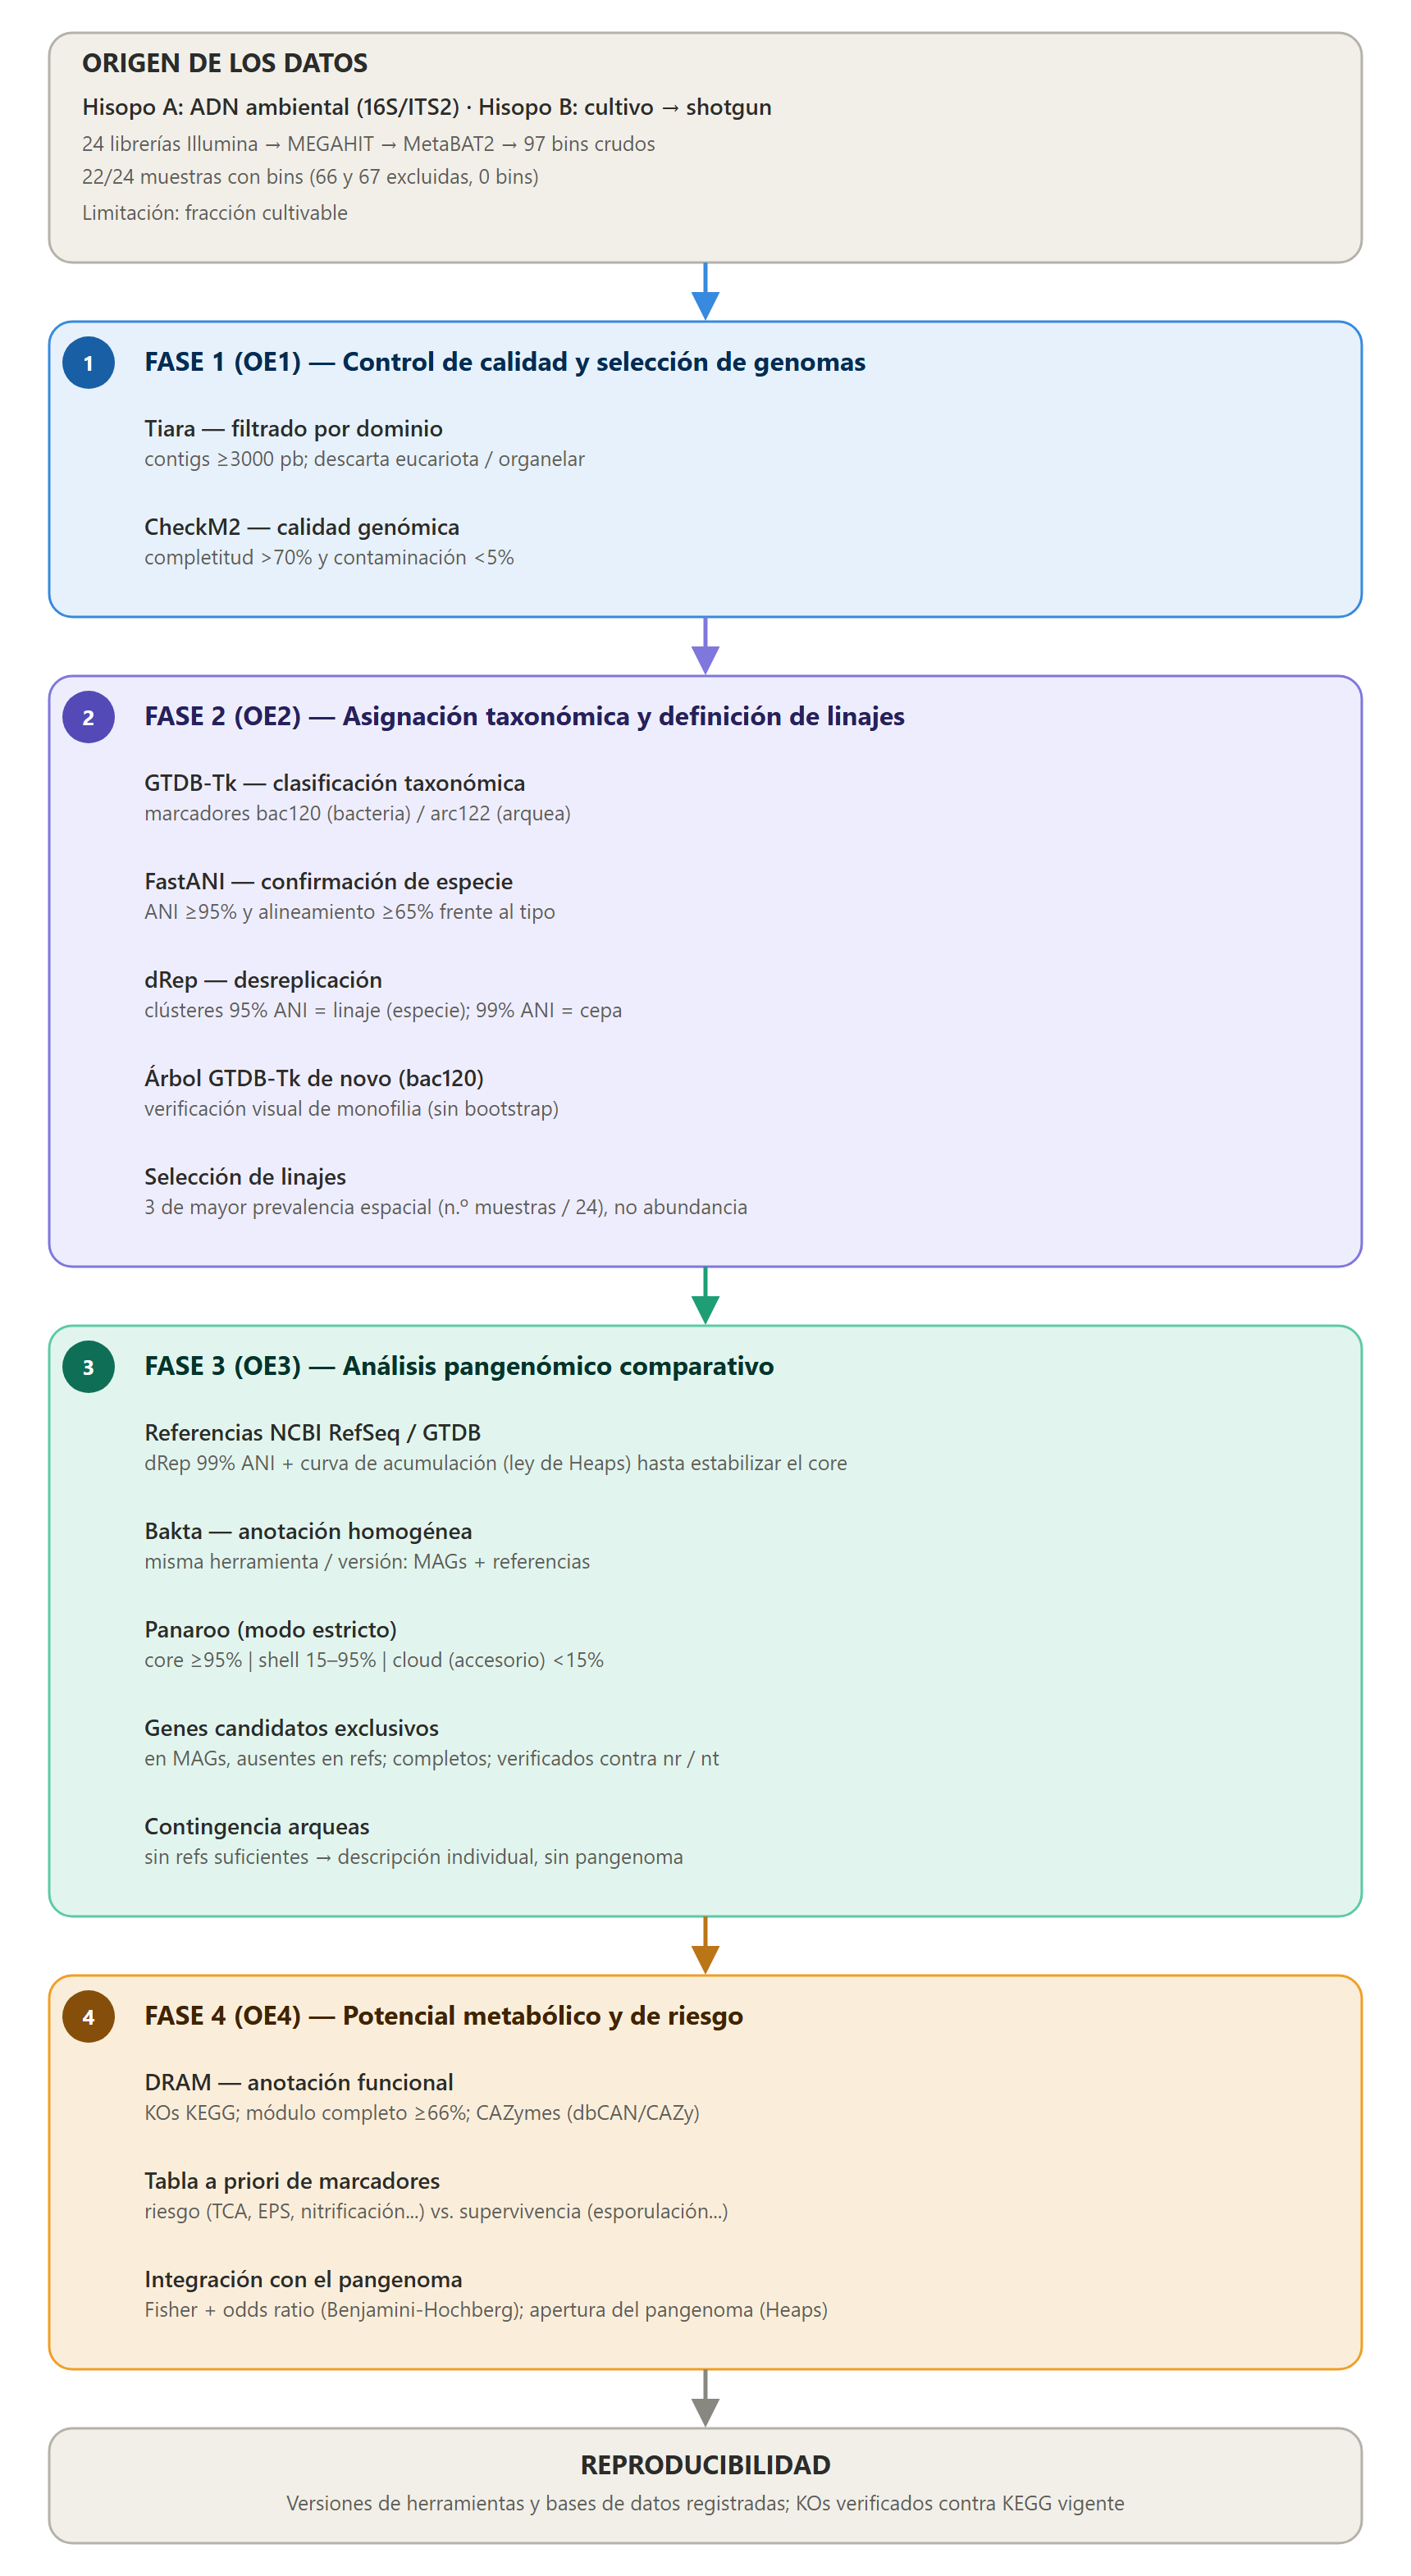
\includegraphics[width=0.8\textwidth]{images/flujograma tesis.png}
    \caption{Flujograma del marco metodológico: cuatro fases consecutivas (OE1 a OE4) desde el origen de los datos metagenómicos hasta la caracterización del potencial metabólico y de riesgo.}
    \label{fig:flujo_metodologico}
\end{figure}


\section*{ANEXO ABET ING 7 --- Aprendizaje continuo}
\addcontentsline{toc}{section}{Aprendizaje continuo}
\renewcommand{\arraystretch}{1.3}
\small
\begin{xltabular}{\textwidth}{|p{1.5cm}|>{\raggedright\arraybackslash}X|>{\raggedright\arraybackslash}p{3cm}|}
\caption{Aprendizaje continuo: fuentes consultadas, contenido aprendido y su aplicación en el documento.}\label{tab:aprendizaje}\\
\hline
\textbf{Ref.} & \textbf{Información o contenido aprendido} & \textbf{Aplicación (en el documento)} \\
\hline
\endfirsthead
\multicolumn{3}{c}{\tablename\ \thetable\ -- continuación}\\
\hline
\textbf{Ref.} & \textbf{Información o contenido aprendido} & \textbf{Aplicación} \\
\hline
\endhead
\hline
\endfoot
\hline
\endlastfoot
~\cite{dakal2012}, ~\cite{li2018deterioration}, ~\cite{chimienti2016}, ~\cite{ding2020preahvihear} & Mecanismos de biodeterioro microbiano de la roca: acidólisis y quelación iónica por ácidos orgánicos de bajo peso molecular, y producción de ácidos nítrico y sulfúrico por bacterias de los ciclos del nitrógeno y del azufre que corroen los minerales. Fundamenta por qué ciertos genes metabólicos implican riesgo material. & Marco Teórico 2.1; Estado del arte; Marco Metodológico \\
\hline
~\cite{villa2016}, ~\cite{PitaGaleana2025}, ~\cite{ding2020}, ~\cite{flemming2010} & Marco ecológico de las biopelículas subaéreas en piedra, arquitectura de la matriz de EPS y rol dual biodeterioro/bioprotección, que motiva pasar de la identidad taxonómica al repertorio funcional. & Formulación del problema; Marco Teórico 2.2; Justificación \\
\hline
~\cite{PitaGaleana2025}, ~\cite{bowers2017} & Flujo de la metagenómica \textit{shotgun}: ensamblaje \textit{de novo} por grafos de De Bruijn y \textit{binning} por composición de tetranucleótidos y cobertura diferencial para reconstruir MAGs. & Formulación del problema; Marco Teórico 2.3; Marco Metodológico\\
\hline
~\cite{checkm2}, ~\cite{bowers2017}, ~\cite{Parks2015} & Definición de completitud y contaminación mediante genes marcadores de copia única; categorías de calidad MIMAG; estimación por aprendizaje automático (CheckM2) sin asignación taxonómica previa. & Marco Teórico 2.4; Marco Metodológico 4.1.3 \\
\hline
~\cite{gtdbtk2019},~\cite{fastANI2018}, ~\cite{gtdb2022}, ~\cite{olm2017} & Clasificación genómica normalizada por divergencia evolutiva (GTDB-Tk/GTDB), delimitación de especie por ANI (umbral del 95\%) y sdereplicación para colapsar genomas redundantes y definir linajes. & Marco Teórico 2.5; Marco Metodológico 4.1.4 \\
\hline
~\cite{panaroo2020},~\cite{tettelin2005} & Concepto de pangenoma y partición en genoma núcleo, cubierta y accesorio; la transferencia horizontal como motor de adaptación; corrección de la inflación del accesorio por fragmentación mediante grafos (Panaroo). & Marco Teórico 2.6; Marco Metodológico 4.1.5 \\
\hline
~\cite{dram2020},~\cite{Hyatt2010}, ~\cite{schwengers2021} & Predicción de ORFs y anotación estandarizada sin alineamiento (Bakta); destilación del metabolismo y cálculo de completitud de módulos/rutas (DRAM) sobre ortólogos KEGG, base para inferir el potencial de biodeterioro. & Marco Teórico 2.7; Marco Metodológico 4.1.6 \\
\hline
~\cite{karlicki2022tiara},~\cite{pronk2022whokaryote}, ~\cite{west2018genomereconstruction} & Clasificadores de contigs por dominio: aprendizaje profundo sobre composición (Tiara), estructura génica con \textit{random forest} (Whokaryote) y \textit{k-mers} con SVM (EukRep); criterios para seleccionar la herramienta de filtrado. & Marco Metodológico 4.1.3.1; Anexo 1 \\
\hline
~\cite{cordycollins1993},~\cite{hernandez2012}, ~\cite{mnaahp2015} & Contexto histórico-arqueológico de la Estela de Raimondi: filiación con la cultura Chavín, hallazgo, traslados sucesivos y custodia museística actual. & Introducción (Presentación del proyecto) \\
\hline
\end{xltabular}

\section{Anexo: Repositorio de GitHub}

Link: \href{https://github.com/EduardoTllo/biodeterioro-estela-pipeline}{GitHub}

\section{Anexo: Reporte completo de calidad y selección de bins (Fase 1)}
\label{anexo:tabla_completa_bins}

\begingroup
\small
\setlength{\tabcolsep}{2.5pt} % Espaciado entre columnas

\begin{xltabular}{\textwidth}{|c|c|c|c|c|c|>{\centering\arraybackslash}X|}
\caption{Reporte completo de evaluación y filtrado de bins genómicos (Fase 1).} \label{anexo:tabla_completa_bins} \\
\hline
\textbf{Bin} & \textbf{Contigs} & \textbf{Long (bp)} & \textbf{Dom.} & \textbf{Comp. (\%)} & \textbf{Contam. (\%)} & \textbf{Motivo} \\
\hline
\endfirsthead

\multicolumn{7}{c}{{\bfseries \tablename\ \thetable{} -- Continuación de la página anterior}} \\
\hline
\textbf{Bin} & \textbf{Contigs} & \textbf{Long (bp)} & \textbf{Dom.} & \textbf{Comp. (\%)} & \textbf{Contam. (\%)} & \textbf{Motivo} \\
\hline
\endhead

\hline
\multicolumn{7}{r}{{Continúa en la siguiente página...}} \\
\hline
\endfoot

\hline
\endlastfoot

bin-1-49 & 87 & 545.053 & euk & -- & -- & dominio mayoritario: euk \\ \hline
bin-1-50 & 224 & 2.609.893 & prok & 62.29 & 2.66 & completitud 62.29 $\le$ 70 \\ \hline
bin-1-51 & 51 & 4.727.435 & prok & 100.00 & 0.00 & - \\ \hline
bin-1-52 & 26 & 415.732 & prok & 6.05 & 0.20 & completitud 6.05 $\le$ 70 \\ \hline
bin-1-53 & 30 & 2.476.631 & prok & 99.84 & 0.12 & - \\ \hline
bin-1-54 & 49 & 4.312.038 & prok & 92.25 & 0.01 & - \\ \hline
bin-1-55 & 247 & 34.242.081 & euk & -- & -- & dominio mayoritario: euk \\ \hline
bin-1-56 & 12 & 230.366 & euk & -- & -- & dominio mayoritario: euk \\ \hline
bin-1-57 & 22 & 4.032.412 & prok & 99.99 & 3.23 & - \\ \hline
bin-1-58 & 4725 & 12.125.594 & unknown & 0.00 & 17.71 & completitud 0.00 $\le$ 70; contaminacion 17.71 $\ge$ 5 \\ \hline
bin-1-59 & 98 & 5.907.869 & prok & 99.97 & 3.07 & - \\ \hline
bin-1-60 & 302 & 8.273.570 & prok & 100.00 & 24.87 & contaminacion 24.87 $\ge$ 5 \\ \hline
bin-1-61 & 448 & 40.131.343 & euk & -- & -- & dominio mayoritario: euk \\ \hline
bin-1-62 & 320 & 7.390.811 & prok & 99.72 & 72.67 & contaminacion 72.67 $\ge$ 5 \\ \hline
bin-1-63 & 162 & 65.185.746 & prok & 84.85 & 39.63 & contaminacion 39.63 $\ge$ 5 \\ \hline
bin-1-64 & 163 & 3.944.265 & prok & 99.84 & 0.59 & - \\ \hline
bin-1-65 & 322 & 29.636.962 & euk & -- & -- & dominio mayoritario: euk \\ \hline
bin-1-68 & 50 & 2.465.224 & prok & 100.00 & 1.79 & - \\ \hline
bin-1-69 & 67 & 251.086 & prok & 6.60 & 0.14 & completitud 6.60 $\le$ 70 \\ \hline
bin-1-70 & 3805 & 494.251.631 & unknown & 31.70 & 28.68 & completitud 31.70 $\le$ 70; contaminacion 28.68 $\ge$ 5 \\ \hline
bin-1-71 & 37 & 11.498.934 & prok & 67.71 & 15.05 & completitud 67.71 $\le$ 70; contaminacion 15.05 $\ge$ 5 \\ \hline
bin-1-72 & 16 & 7.408.652 & unknown & 5.87 & 0.19 & completitud 5.87 $\le$ 70 \\ \hline
bin-10-71 & 506 & 2.845.557 & prok & 97.57 & 30.13 & contaminacion 30.13 $\ge$ 5 \\ \hline
bin-11-71 & 4161 & 101.946.556 & unknown & 65.68 & 17.72 & completitud 65.68 $\le$ 70; contaminacion 17.72 $\ge$ 5 \\ \hline
bin-12-71 & 383 & 1.015.904 & unknown & 43.42 & 3.52 & completitud 43.42 $\le$ 70 \\ \hline
bin-2-49 & 134 & 27.557.437 & euk & -- & -- & dominio mayoritario: euk \\ \hline
bin-2-50 & 464 & 53.406.620 & euk & -- & -- & dominio mayoritario: euk \\ \hline
bin-2-52 & 270 & 5.347.688 & prok & 99.93 & 8.10 & contaminacion 8.10 $\ge$ 5 \\ \hline
bin-2-53 & 39 & 5.164.804 & prok & 99.99 & 0.57 & - \\ \hline
bin-2-54 & 106 & 7.273.841 & prok & 100.00 & 15.52 & contaminacion 15.52 $\ge$ 5 \\ \hline
bin-2-56 & 816 & 49.647.189 & euk & -- & -- & dominio mayoritario: euk \\ \hline
bin-2-57 & 28 & 5.172.263 & prok & 99.96 & 1.01 & - \\ \hline
bin-2-58 & 17 & 4.771.531 & prok & 100.00 & 0.06 & - \\ \hline
bin-2-59 & 424 & 23.212.147 & prok & 91.94 & 115.89 & contaminacion 115.89 $\ge$ 5 \\ \hline
bin-2-60 & 290 & 10.390.751 & prok & 100.00 & 100.33 & contaminacion 100.33 $\ge$ 5 \\ \hline
bin-2-61 & 9 & 614.253 & euk & -- & -- & dominio mayoritario: euk \\ \hline
bin-2-62 & 5 & 227.679 & euk & -- & -- & dominio mayoritario: euk \\ \hline
bin-2-63 & 150 & 4.282.638 & prok & 92.39 & 0.34 & - \\ \hline
bin-2-64 & 924 & 226.083.286 & unknown & 0.02 & 16.03 & completitud 0.02 $\le$ 70; contaminacion 16.03 $\ge$ 5 \\ \hline
bin-2-65 & 141 & 17.056.380 & euk & -- & -- & dominio mayoritario: euk \\ \hline
bin-2-68 & 70 & 246.182 & prok & 4.99 & 0.03 & completitud 4.99 $\le$ 70 \\ \hline
bin-2-69 & 61 & 2.481.071 & prok & 99.99 & 0.18 & - \\ \hline
bin-2-70 & 87 & 278.635 & unknown & 5.38 & 0.09 & completitud 5.38 $\le$ 70 \\ \hline
bin-2-71 & 618 & 1.368.774 & unknown & 56.83 & 26.01 & completitud 56.83 $\le$ 70; contaminacion 26.01 $\ge$ 5 \\ \hline
bin-2-72 & 667 & 2.485.725 & prok & 79.16 & 54.30 & contaminacion 54.30 $\ge$ 5 \\ \hline
bin-3-50 & 30 & 2.607.902 & unknown & 13.03 & 0.08 & completitud 13.03 $\le$ 70 \\ \hline
bin-3-52 & 204 & 5.184.467 & prok & 98.97 & 0.58 & - \\ \hline
bin-3-53 & 301 & 29.244.092 & euk & -- & -- & dominio mayoritario: euk \\ \hline
bin-3-56 & 160 & 26.628.065 & euk & -- & -- & dominio mayoritario: euk \\ \hline
bin-3-57 & 818 & 25.745.728 & euk & -- & -- & dominio mayoritario: euk \\ \hline
bin-3-58 & 265 & 29.647.785 & euk & -- & -- & dominio mayoritario: euk \\ \hline
bin-3-60 & 959 & 2.321.293 & unknown & 39.27 & 0.00 & completitud 39.27 $\le$ 70 \\ \hline
bin-3-61 & 50 & 10.715.439 & euk & -- & -- & dominio mayoritario: euk \\ \hline
bin-3-62 & 117 & 449.659 & euk & -- & -- & dominio mayoritario: euk \\ \hline
bin-3-63 & 4589 & 19.740.558 & prok & 99.91 & 102.18 & contaminacion 102.18 $\ge$ 5 \\ \hline
bin-3-64 & 459 & 2.352.198 & prok & 70.14 & 0.64 & - \\ \hline
bin-3-65 & 5256 & 27.711.612 & euk & -- & -- & dominio mayoritario: euk \\ \hline
bin-3-70 & 169 & 64.261.799 & unknown & 77.48 & 75.48 & contaminacion 75.48 $\ge$ 5 \\ \hline
bin-3-71 & 3657 & 12.324.162 & prok & 97.39 & 70.70 & contaminacion 70.70 $\ge$ 5 \\ \hline
bin-3-72 & 174 & 16.597.747 & prok & 98.53 & 98.35 & contaminacion 98.35 $\ge$ 5 \\ \hline
bin-4-50 & 97 & 1.654.013 & prok & 43.00 & 0.23 & completitud 43.00 $\le$ 70 \\ \hline
bin-4-52 & 96 & 3.497.259 & prok & 99.86 & 0.25 & - \\ \hline
bin-4-56 & 122 & 1.739.035 & euk & -- & -- & dominio mayoritario: euk \\ \hline
bin-4-57 & 977 & 39.075.173 & euk & -- & -- & dominio mayoritario: euk \\ \hline
bin-4-60 & 4482 & 25.724.799 & euk & -- & -- & dominio mayoritario: euk \\ \hline
bin-4-61 & 1610 & 11.012.084 & prok & 100.00 & 58.51 & contaminacion 58.51 $\ge$ 5 \\ \hline
bin-4-62 & 270 & 79.759.046 & prok & 90.25 & 65.70 & contaminacion 65.70 $\ge$ 5 \\ \hline
bin-4-63 & 856 & 56.508.797 & euk & -- & -- & dominio mayoritario: euk \\ \hline
bin-4-64 & 428 & 29.693.972 & euk & -- & -- & dominio mayoritario: euk \\ \hline
bin-4-65 & 2506 & 20.150.702 & prok & 99.99 & 106.28 & contaminacion 106.28 $\ge$ 5 \\ \hline
bin-4-70 & 484 & 1.565.460 & prok & 64.00 & 2.55 & completitud 64.00 $\le$ 70 \\ \hline
bin-4-71 & 216 & 488.562 & unknown & 32.24 & 2.32 & completitud 32.24 $\le$ 70 \\ \hline
bin-4-72 & 72 & 248.801 & prok & 4.69 & 0.01 & completitud 4.69 $\le$ 70 \\ \hline
bin-5-50 & 1041 & 3.472.002 & prok & 76.56 & 0.44 & - \\ \hline
bin-5-52 & 1099 & 3.740.736 & prok & 95.51 & 12.95 & contaminacion 12.95 $\ge$ 5 \\ \hline
bin-5-56 & 146 & 552.204 & euk & -- & -- & dominio mayoritario: euk \\ \hline
bin-5-57 & 12 & 224.138 & euk & -- & -- & dominio mayoritario: euk \\ \hline
bin-5-60 & 97 & 2.849.856 & prok & 77.53 & 0.10 & - \\ \hline
bin-5-61 & 273 & 5.811.268 & prok & 97.82 & 10.64 & contaminacion 10.64 $\ge$ 5 \\ \hline
bin-5-62 & 222 & 27.886.446 & euk & -- & -- & dominio mayoritario: euk \\ \hline
bin-5-63 & 90 & 2.758.939 & prok & 72.46 & 0.05 & - \\ \hline
bin-5-64 & 217 & 39.450.268 & prok & 100.00 & 67.99 & contaminacion 67.99 $\ge$ 5 \\ \hline
bin-5-65 & 24 & 222.213 & euk & -- & -- & dominio mayoritario: euk \\ \hline
bin-5-70 & 28 & 2.628.283 & unknown & 48.48 & 2.40 & completitud 48.48 $\le$ 70 \\ \hline
bin-5-71 & 118 & 438.388 & prok & 12.74 & 0.54 & completitud 12.74 $\le$ 70 \\ \hline
bin-6-50 & 591 & 5.543.214 & prok & 100.00 & 0.65 & - \\ \hline
bin-6-56 & 116 & 9.578.458 & euk & -- & -- & dominio mayoritario: euk \\ \hline
bin-6-57 & 126 & 448.524 & euk & -- & -- & dominio mayoritario: euk \\ \hline
bin-6-61 & 30 & 4.792.746 & prok & 100.00 & 0.74 & - \\ \hline
bin-6-63 & 21 & 367.167 & euk & -- & -- & dominio mayoritario: euk \\ \hline
bin-6-64 & 71 & 239.057 & euk & -- & -- & dominio mayoritario: euk \\ \hline
bin-6-70 & 319 & 48.190.971 & unknown & 68.24 & 17.99 & completitud 68.24 $\le$ 70; contaminacion 17.99 $\ge$ 5 \\ \hline
bin-6-71 & 34 & 453.921 & prok & 11.79 & 0.16 & completitud 11.79 $\le$ 70 \\ \hline
bin-7-64 & 1246 & 3.769.741 & prok & 60.17 & 0.22 & completitud 60.17 $\le$ 70 \\ \hline
bin-7-71 & 95 & 258.968 & unknown & 7.21 & 0.05 & completitud 7.21 $\le$ 70 \\ \hline
bin-8-71 & 908 & 2.450.575 & unknown & 81.92 & 35.87 & contaminacion 35.87 $\ge$ 5 \\ \hline
bin-9-71 & 346 & 1.832.072 & prok & 85.09 & 2.13 & - \\
\end{xltabular}
\endgroup

\end{document}
